\documentclass[a4paper,11pt]{report}

\usepackage{report}
\usepackage[utf8]{inputenc} % allow utf-8 input
\usepackage[T1]{fontenc}    % use 8-bit T1 fonts
% \usepackage[colorlinks=true, linkcolor=black, citecolor=blue, urlcolor=blue]{hyperref}       % hyperlinks
\usepackage[colorlinks=true, linkcolor=black, citecolor=black, urlcolor=black]{hyperref}       % hyperlinks
\usepackage{url}            % simple URL typesetting
\usepackage{booktabs}       % professional-quality tables
\usepackage{amsfonts}       % blackboard math symbols
\usepackage{nicefrac}       % compact symbols for 1/2, etc.
\usepackage{microtype}      % microtypography
\usepackage{graphicx}
\usepackage{doi}
\usepackage{tikz}
\usepackage{amsmath}
\usepackage{amssymb}
\usepackage{chemformula}
\usepackage{listings}
\usepackage{xcolor}
\usepackage{mwe}
\usepackage{siunitx}
\usepackage{appendix}
\usepackage{setspace}
\usepackage{subcaption}
\usepackage{cprotect}
\usepackage[super]{nth}
\usepackage{cite}


\usepackage[capitalise]{cleveref}
\creflabelformat{equation}{#2\textup{#1}#3}
\usepackage{amsthm}

\DeclareSIUnit\eVperc{\eV\per\clight}
\DeclareSIUnit\clight{\text{\ensuremath{c}}}

\makeatletter
  \renewcommand*\tagform@[1]{\maketag@@@{Eq.~\ignorespaces #1\unskip\@@italiccorr}}
\makeatother


\definecolor{codegreen}{rgb}{0,0.6,0}
\definecolor{codegray}{rgb}{0.5,0.5,0.5}
\definecolor{codepurple}{rgb}{0.58,0,0.82}
\definecolor{backcolour}{rgb}{0.95,0.95,0.92}

\newcommand{\hly}[1]{\colorbox{yellow}{\parbox{\textwidth}{#1}}}
\newcommand\todo[1]{\textcolor{red}{#1}}

\lstdefinestyle{mystyle}{
    backgroundcolor=\color{backcolour},   
    commentstyle=\color{codegreen},
    keywordstyle=\color{magenta},
    numberstyle=\tiny\color{codegray},
    stringstyle=\color{codepurple},
    basicstyle=\ttfamily\footnotesize,
    breakatwhitespace=false,         
    breaklines=true,                 
    captionpos=b,                    
    keepspaces=true,                 
    numbers=left,                    
    numbersep=5pt,                  
    showspaces=false,                
    showstringspaces=false,
    showtabs=false,                  
    tabsize=2
}

\lstset{style=mystyle}

%% ========================
%% [TODO)
%% REMOVE BEFORE SUBMISSION
 \usepackage[angle=0, fontsize=0.04\paperwidth, vpos=0.027\paperheight, color=gray, text=DRAFT\ Aug\ 22]{draftwatermark}
%% ========================
% BUG

%\setcitestyle{aysep={,}}
%\renewcommand{\headeright}{M.Sc. Thesis}
\renewcommand{\headeright}{\textsc{\rightmark}}
\renewcommand{\shorttitle}{}


\setlength{\parindent}{20pt}
\onehalfspacing
\begin{document}
%%%%%%%%%%%%%%%%%%%%%%%%%%%%%%%%%%%%%%%%%
% University Assignment Title Page 
% LaTeX Template
% Version 1.0 (27/12/12)
%
% This template has been downloaded from:
% http://www.LaTeXTemplates.com
%
% Original author:
% WikiBooks (http://en.wikibooks.org/wiki/LaTeX/Title_Creation)
%
% License:
% CC BY-NC-SA 3.0 (http://creativecommons.org/licenses/by-nc-sa/3.0/)
% 
% Instructions for using this template:
% This title page is capable of being compiled as is. This is not useful for 
% including it in another document. To do this, you have two options: 
%
% 1) Copy/paste everything between \begin{document} and \end{document} 
% starting at \begin{titlepage} and paste this into another LaTeX file where you 
% want your title page.
% OR
% 2) Remove everything outside the \begin{titlepage} and \end{titlepage} and 
% move this file to the same directory as the LaTeX file you wish to add it to. 
% Then add \input{./title_page_1.tex} to your LaTeX file where you want your
% title page.
%
%%%%%%%%%%%%%%%%%%%%%%%%%%%%%%%%%%%%%%%%%
%\title{Title page with logo}
%----------------------------------------------------------------------------------------
%	PACKAGES AND OTHER DOCUMENT CONFIGURATIONS
%----------------------------------------------------------------------------------------
\begin{titlepage}

\newcommand{\HRule}{\rule{\linewidth}{0.5mm}} % Defines a new command for the horizontal lines, change thickness here
\center % Center everything on the page
 
%----------------------------------------------------------------------------------------
%	HEADING SECTIONS
%----------------------------------------------------------------------------------------

\textsc{\LARGE Royal Holloway University of London}\\[1.5cm] % Name of your university/college
\textsc{\Large M.Sc Thesis}\\[0.5cm] % Major heading such as course name
\textsc{\large Student ID: 100920158}\\[0.5cm] % Minor heading such as course title

%----------------------------------------------------------------------------------------
%	TITLE SECTION
%----------------------------------------------------------------------------------------

\HRule \\[0.4cm]
\begin{spacing}{2}
{ \huge \bfseries Comparative Analysis of Simulations and Experimental Outcomes: Slow Extraction Driven by RF Transverse Excitation at the CERN Proton Synchrotron}\\[0.4cm] % Title of your document
\end{spacing}
\HRule \\[0.4cm]

 
%----------------------------------------------------------------------------------------
%	AUTHOR SECTION
%----------------------------------------------------------------------------------------

\begin{minipage}{0.4\textwidth}
\begin{flushleft} \large
\emph{Author:}\\
Thomas \textsc{Bass} % Your name
\end{flushleft}
\end{minipage}
~
\begin{minipage}{0.4\textwidth}
\begin{flushright} \large
\emph{Supervisor:} \\
Professor Stephen \textsc{Gibson} % Supervisor's Name
\end{flushright}
\end{minipage}\\[2cm]

% If you don't want a supervisor, uncomment the two lines below and remove the section above
%\Large \emph{Author:}\\
%John \textsc{Smith}\\[3cm] % Your name

%----------------------------------------------------------------------------------------
%	DATE SECTION
%----------------------------------------------------------------------------------------

{\large \today}\\[2cm] % Date, change the \today to a set date if you want to be precise

%----------------------------------------------------------------------------------------
%	LOGO SECTION
%----------------------------------------------------------------------------------------


\includegraphics[width=0.25\linewidth]{Royal_Holloway_coat_of_arms.png}\\[1cm] % Include a department/university logo - this will require the graphicx package
 
%----------------------------------------------------------------------------------------

\vfill % Fill the rest of the page with whitespace

\end{titlepage}


\newpage
\thispagestyle{empty}
\vspace*{\fill}
\begin{center}
    \textbf{Declaration of Authorship}
\end{center}
I hereby declare that this thesis and the work presented in it are entirely my own. Where I have consulted the published work of others, this is always clearly attributed. \\[4pt]
\\[4pt]


\begin{tabbing}
\textbf{Thomas Bass} \\[16pt]
\includegraphics*[width=0.2\linewidth]{signature.png} \\[8pt]
\textbf{Date:} \text{18th September 2023} \\
\end{tabbing}
\vspace*{\fill}

This project has received funding from the European Union's Horizon 2020 Research and Innovation programme under grant agreement Number 101004730.
\vspace*{\fill}
\newpage
\thispagestyle{empty}
\begin{abstract}
  \setlength{\parindent}{20pt}
Radio-Frequency Knockout (RFKO) is a method of resonant slow beam extraction which is able to produce continuous particle spills over durations longer than can be achieved with fast single-turn or non-resonant multi-turn extraction. By using transverse excitation to gradually drive the circulating particles into resonance, spills can be produced over many thousands of turns, at a low intensity, and with a flat time profile.These spills can be delivered to facilities---such as fixed-target experiments or hadron therapy gantries---which require a continuous, low-intensity particle flux of durations significantly longer than the particle revolution period.

In order to accurately and efficiently simulate this extraction process over a wide range of timescales, new modelling tools and computing platforms must be explored. By utilising optimised computational hardware---such as General Purpose Graphics Processing Units (GPGPUs), and next-generation simulation software (such as \verb|Xsuite|), computation times for simulations can be reduced by several orders of magnitude while remaining accurate compared to empirical measurements.

This thesis presents the novel implementation and simulation of RFKO slow extraction at the East Area (EA) experimental facility, located at CERN's Proton Synchrotron (PS). The results of the experiments outlined seek to confirm both the accuracy of the simulated frequency response and time structure, and the benefits of GPU-accelerated simulation software. These results will also provide an analysis of optimal parameter selections for both the extraction control system---optimising for spill quality---and the simulation system architecture---optimising for performance.

\end{abstract}
\vspace*{\fill}
\keywords{Beam Physics, Computational Physics, Slow Extraction, Radio-Frequency Knockout, Simulation, Xsuite}
\vspace*{\fill}


\newpage
\tableofcontents
\listoffigures
\listoftables
\newpage

\chapter{Introduction}

The CERN Proton Synchrotron (PS), alongside providing intermediary acceleration for hadron and ion beams for the Super Proton Synchrotron (SPS) and eventually the Large Hadron Collider (LHC), provides beams for the many fixed target experiments located at the East Area (EA) experimental facility. This facility, as illustrated in~\autoref{fig:eadiagram}, consists of the proton (IRRAD) and mixed-field (CHARM) irradiation facilities, via a dedicated \qty{24}{GeV/c} beamline, in addition to a multi-target beamline providing three secondary beams.

Ongoing experiments in these facilities such as the CHARM High-energy Ions for Micro Electronics Reliability Assurance (CHIMERA)~\cite{Fraser:feasibility} use high-Z ions (Pb) to simulate the harsh radiation environment of cosmic rays which satellites experience. Using low-intensity (\qty{<e6}{ions/spill}), high-energy (\qty{>100}{\MeV / u}) beams, customers such as the European Space Agency can assess the reliability of new materials in these environments.~\autoref{fig:chain} illustrates the two injection chains of the PS, either with Lead ions sourced from the Linear Accelerator 3 (Linac3) and Low Energy Ion Ring (LEIR) chain, or protons from the Linac4 and the Proton Synchrotron Booster (PSB).

\begin{figure}
  \centering
  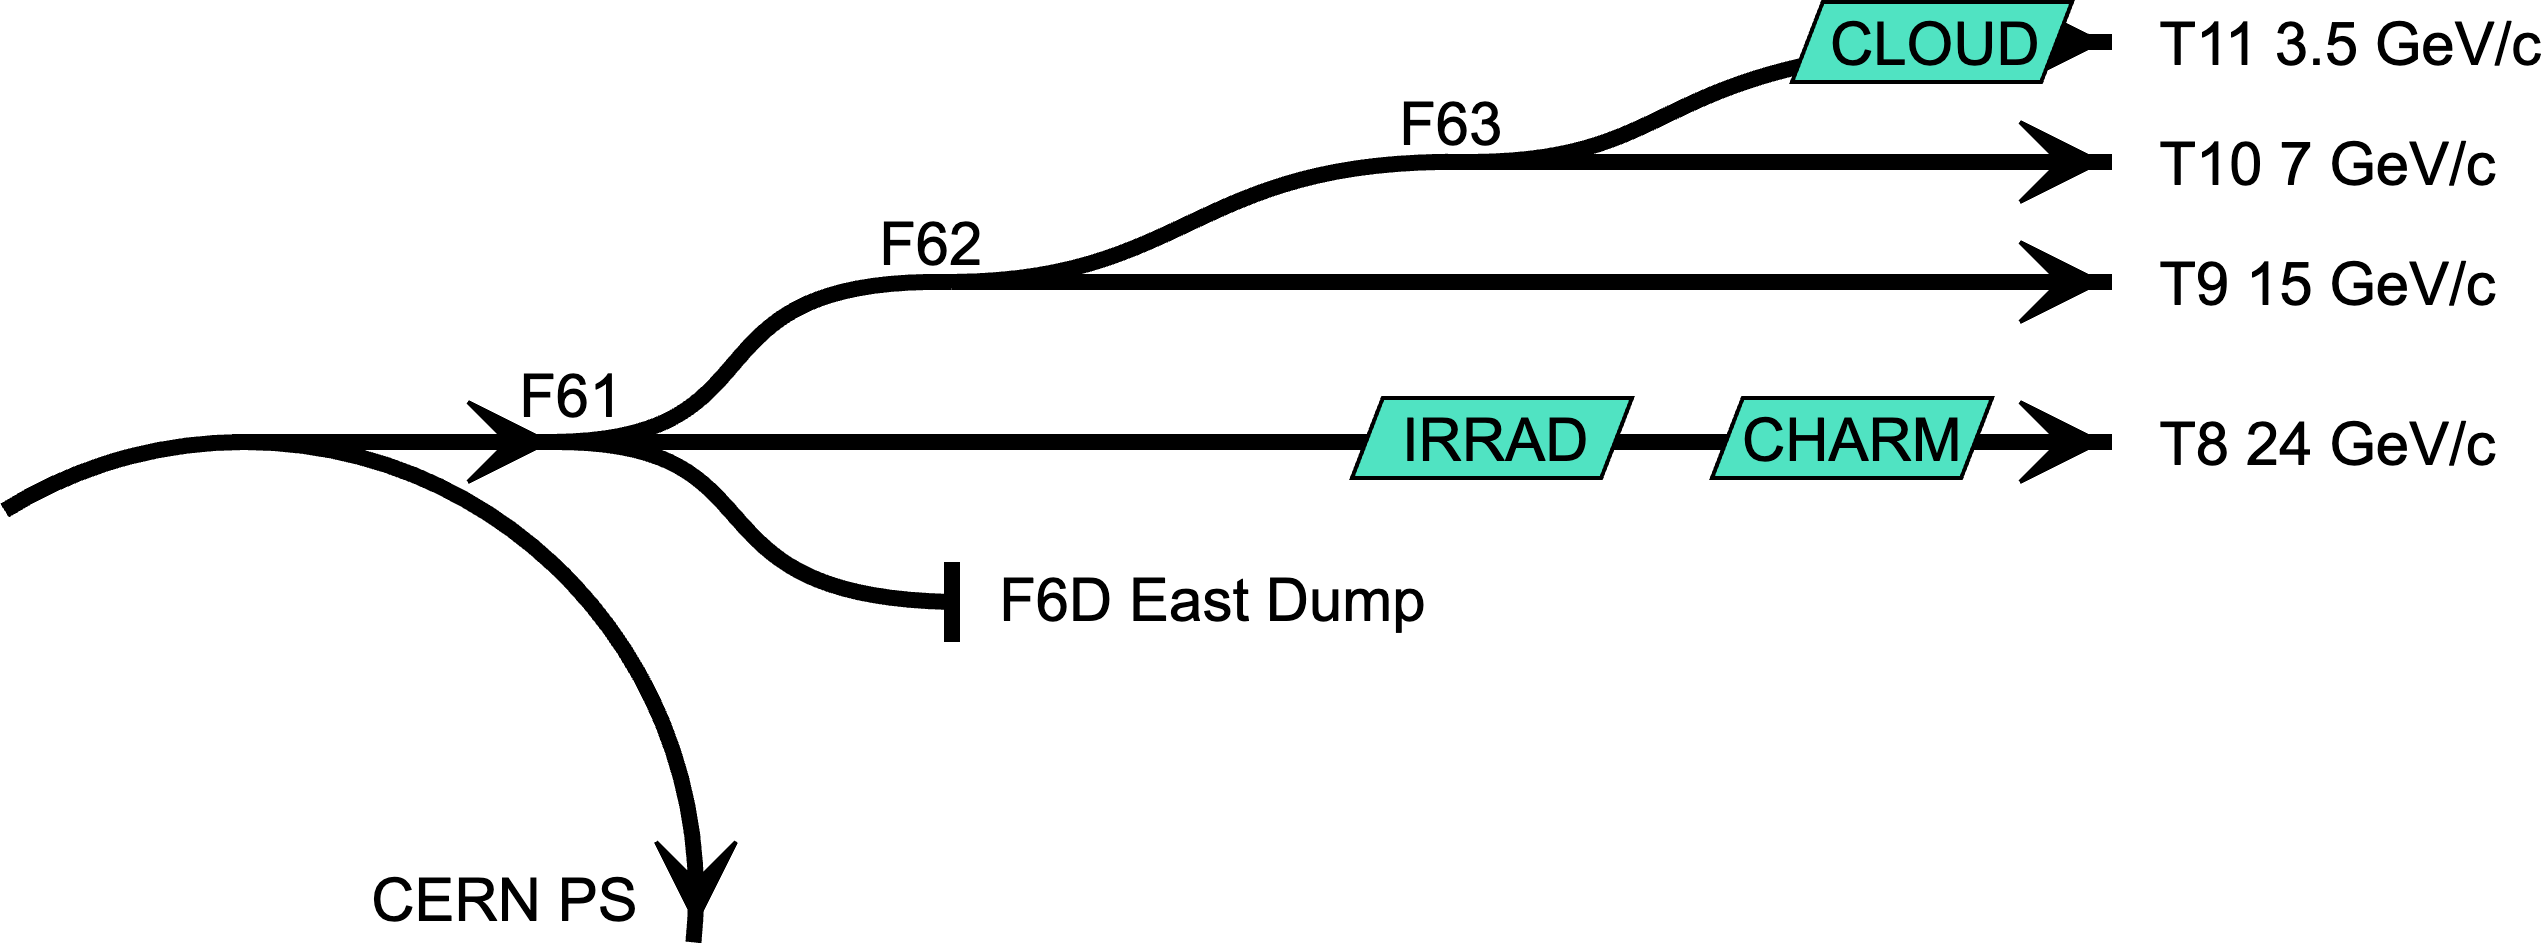
\includegraphics[width=\linewidth]{east-area.png}
  \caption[Layout of the CERN East Area beamlines]{Layout diagram of the CERN East Area (EA) beamlines, their proton momenta, and experiments.}\label{fig:eadiagram}
\end{figure}

\begin{figure}
  \centering
  \includegraphics*[width=0.8\linewidth]{complex.png}
  \caption[Layout of the primary injectors and accelerators of the CERN complex]{Layout diagram of the primary injection chain at CERN. Particles are sourced from either Linac 3 (for Lead ions) or Linac 4 (for Protons), and accelerated through the LEIR or PSB respectively. After injection and acceleration in the PS, beams are extracted either to the SPS or East Area (EA). Particles at the SPS are either extracted at two LHC extraction locations, or towards the North area. Red diamonds indicate Fast extraction locations, and blue indicate mark Slow extraction regions. Grey triangles indicate injection regions.}\label{fig:chain}
\end{figure}

\section{Motivation}\label{sec:motivation}

The CHIMERA experiment, and other experiments located at the East Area and its higher-energy sister site at the SPS North Area, are referred to as fixed-target experiments. These experiments require a semi-continuous flux of particles at lower intensities than produced by the PS. For example, if the entire beam of the PS was delivered to a material sample in an effectively instantaneous ``spill'' (a controlled removal of particles from the circular accelerator), any sensitive acquisition equipment would become saturated, and the fixed target itself likely destroyed.

At a beam momentum of \qty{5.4}{\giga\electronvolt} in the PS, the revolution frequency of the beam is around \qty{470}{kHz}. Therefore, delivering particles over the period of one turn could, at most, provide a spill time on the order of \qty{2}{\micro\second}. This extraction method, known as \textit{fast} extraction, is commonly used to transfer particles between successive accelerators where the bunched time-structure of the beam is preserved. To provide spills on the order of $\sim$\qty{100}{\ms} required for these experiments, much longer than the revolution period, a ``slow'' extraction system is employed.

\subsection{Extraction Methods}

To move particles between consecutive machines along the primary CERN injector chain, the PSB, PS, and SPS are equipped with fast extraction systems. The principles of these processes will be fully explored in the next section, but a general overview and understanding of its benefits and disadvantages help in understanding the motivation for the use of \textit{slow} extraction.

As previously mentioned, \textit{fast} extraction provides a spill of particles typically over the duration of one turn. A fast magnet, at a suitable location in the machine, imparts a large deflective angle to the beam. This ejects the beam from the nominal orbit, where it encounters a second magnet---called a septum---to deflect the beam into a transfer line. The opposite effect is then used to inject the bunch into the next machine: a magnet ``kicks'' the particles onto the circulating beam trajectory.

\begin{figure}[h]
  \centering
  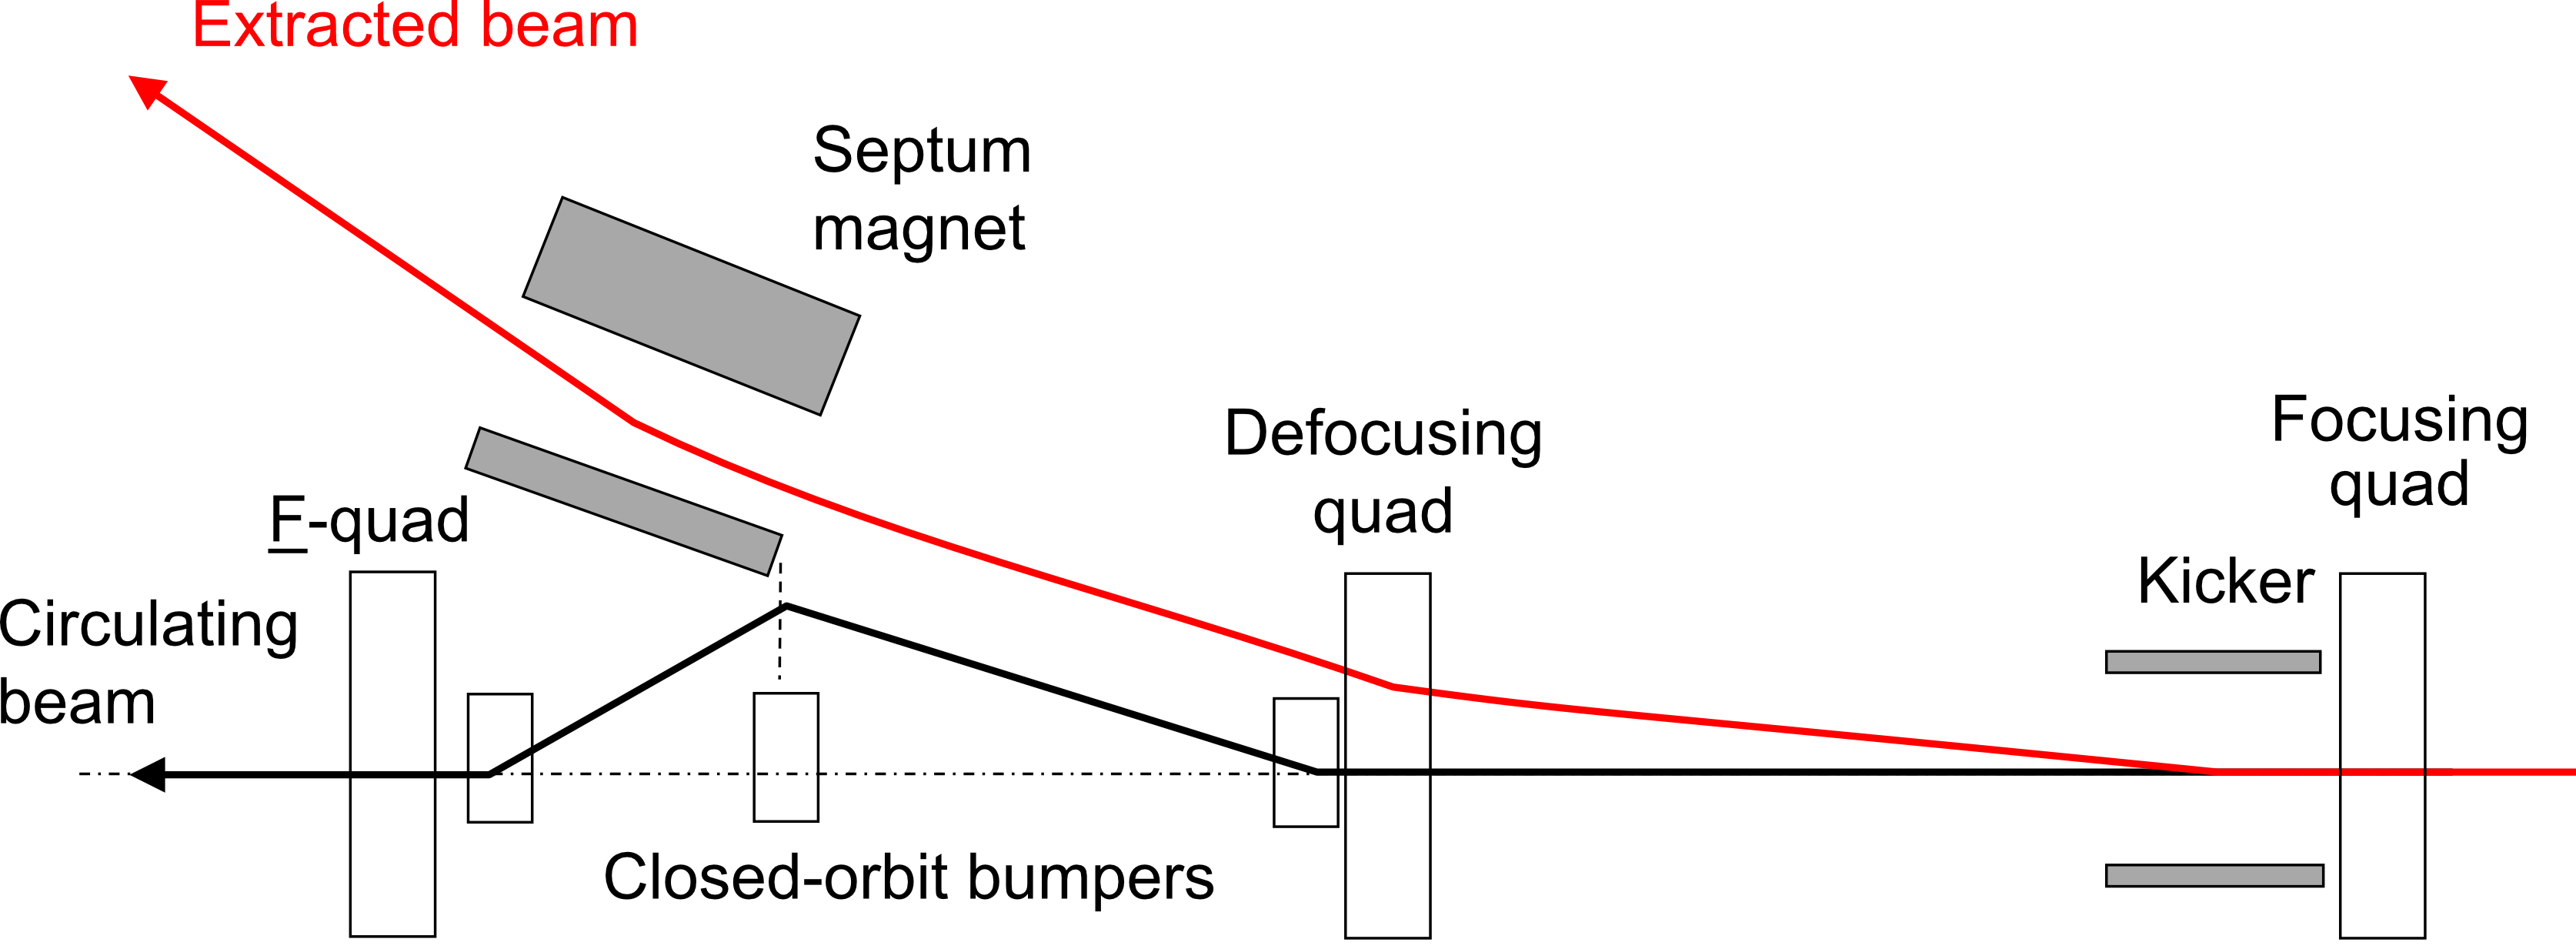
\includegraphics[width=\linewidth]{fast.png}
  \caption{Schematic of the general principle of single-turn fast extraction~\cite{Fraser:CAS}.}\label{fig:fast_diagram}
\end{figure}

This method of \textbf{\textit{single-turn} fast extraction} (~\autoref{fig:fast_diagram}) is used at two locations in the SPS---Long Straight Sections (LSS) 4 and 6---to fill the two counter-rotating rings in the LHC~\cite{Fraser:CAS}. The PSB uses the same method, but has the added complexity of ``merging'' four seperate stacked rings to one transfer line~\cite{Metzmacher:2061508}. LEIR likewise performs fast extraction~\cite{Ghithan:2017wpd}. The general layout of these systems are shown in~\ref{fig:chain}, where red diamonds indicate fast extraction locations. Fast extraction systems are also used at the beam dump facilities at various stages of the accelerator chain to discard the circulating beam at the SPS and LHC.

In accelerator-to-accelerator contexts, the synchronous nature of fast extraction allows particles to remain bunched.~\textbf{Multi-turn fast extraction} extends this benefit, and is performed when filling the SPS for its fixed-target experiments (North Area) from the PS. As the SPS (\qty{6.9}{km}) is approximately 11 times longer in circumference than the PS\footnote{The PS is 100 meters across, and therefore $200\pi$\si{m}} (\qty{628}{m}), the entire SPS can be filled by 11 successive extractions of the full PS. This method, known as \textit{continuous transfer} (CT), introduces the concept of ``shaving'' the beam with an electrostatic septum~\cite{PhysRevSTAB.14.030101}. Previously implemented in extraction from the PS, the beam orbit was bumped similarly to single-turn fast extraction, but was instead forced over the blade of an electrostatic septum (ES), such that a segment the beam is `sliced' off, kicked towards a magnetic septum (MS), and extracted. The remaining beam is then kicked back onto its orbit. After the next turn, the beam has been ``rotated'' by a quarter turn, and the process repeats, until finally the remaining core of the beam is bumped directly to the magnetic septum. This provides a spill to the SPS of five bunches over five beam rotations from a single PS bunch.

\begin{figure}[hb]
  \centering
  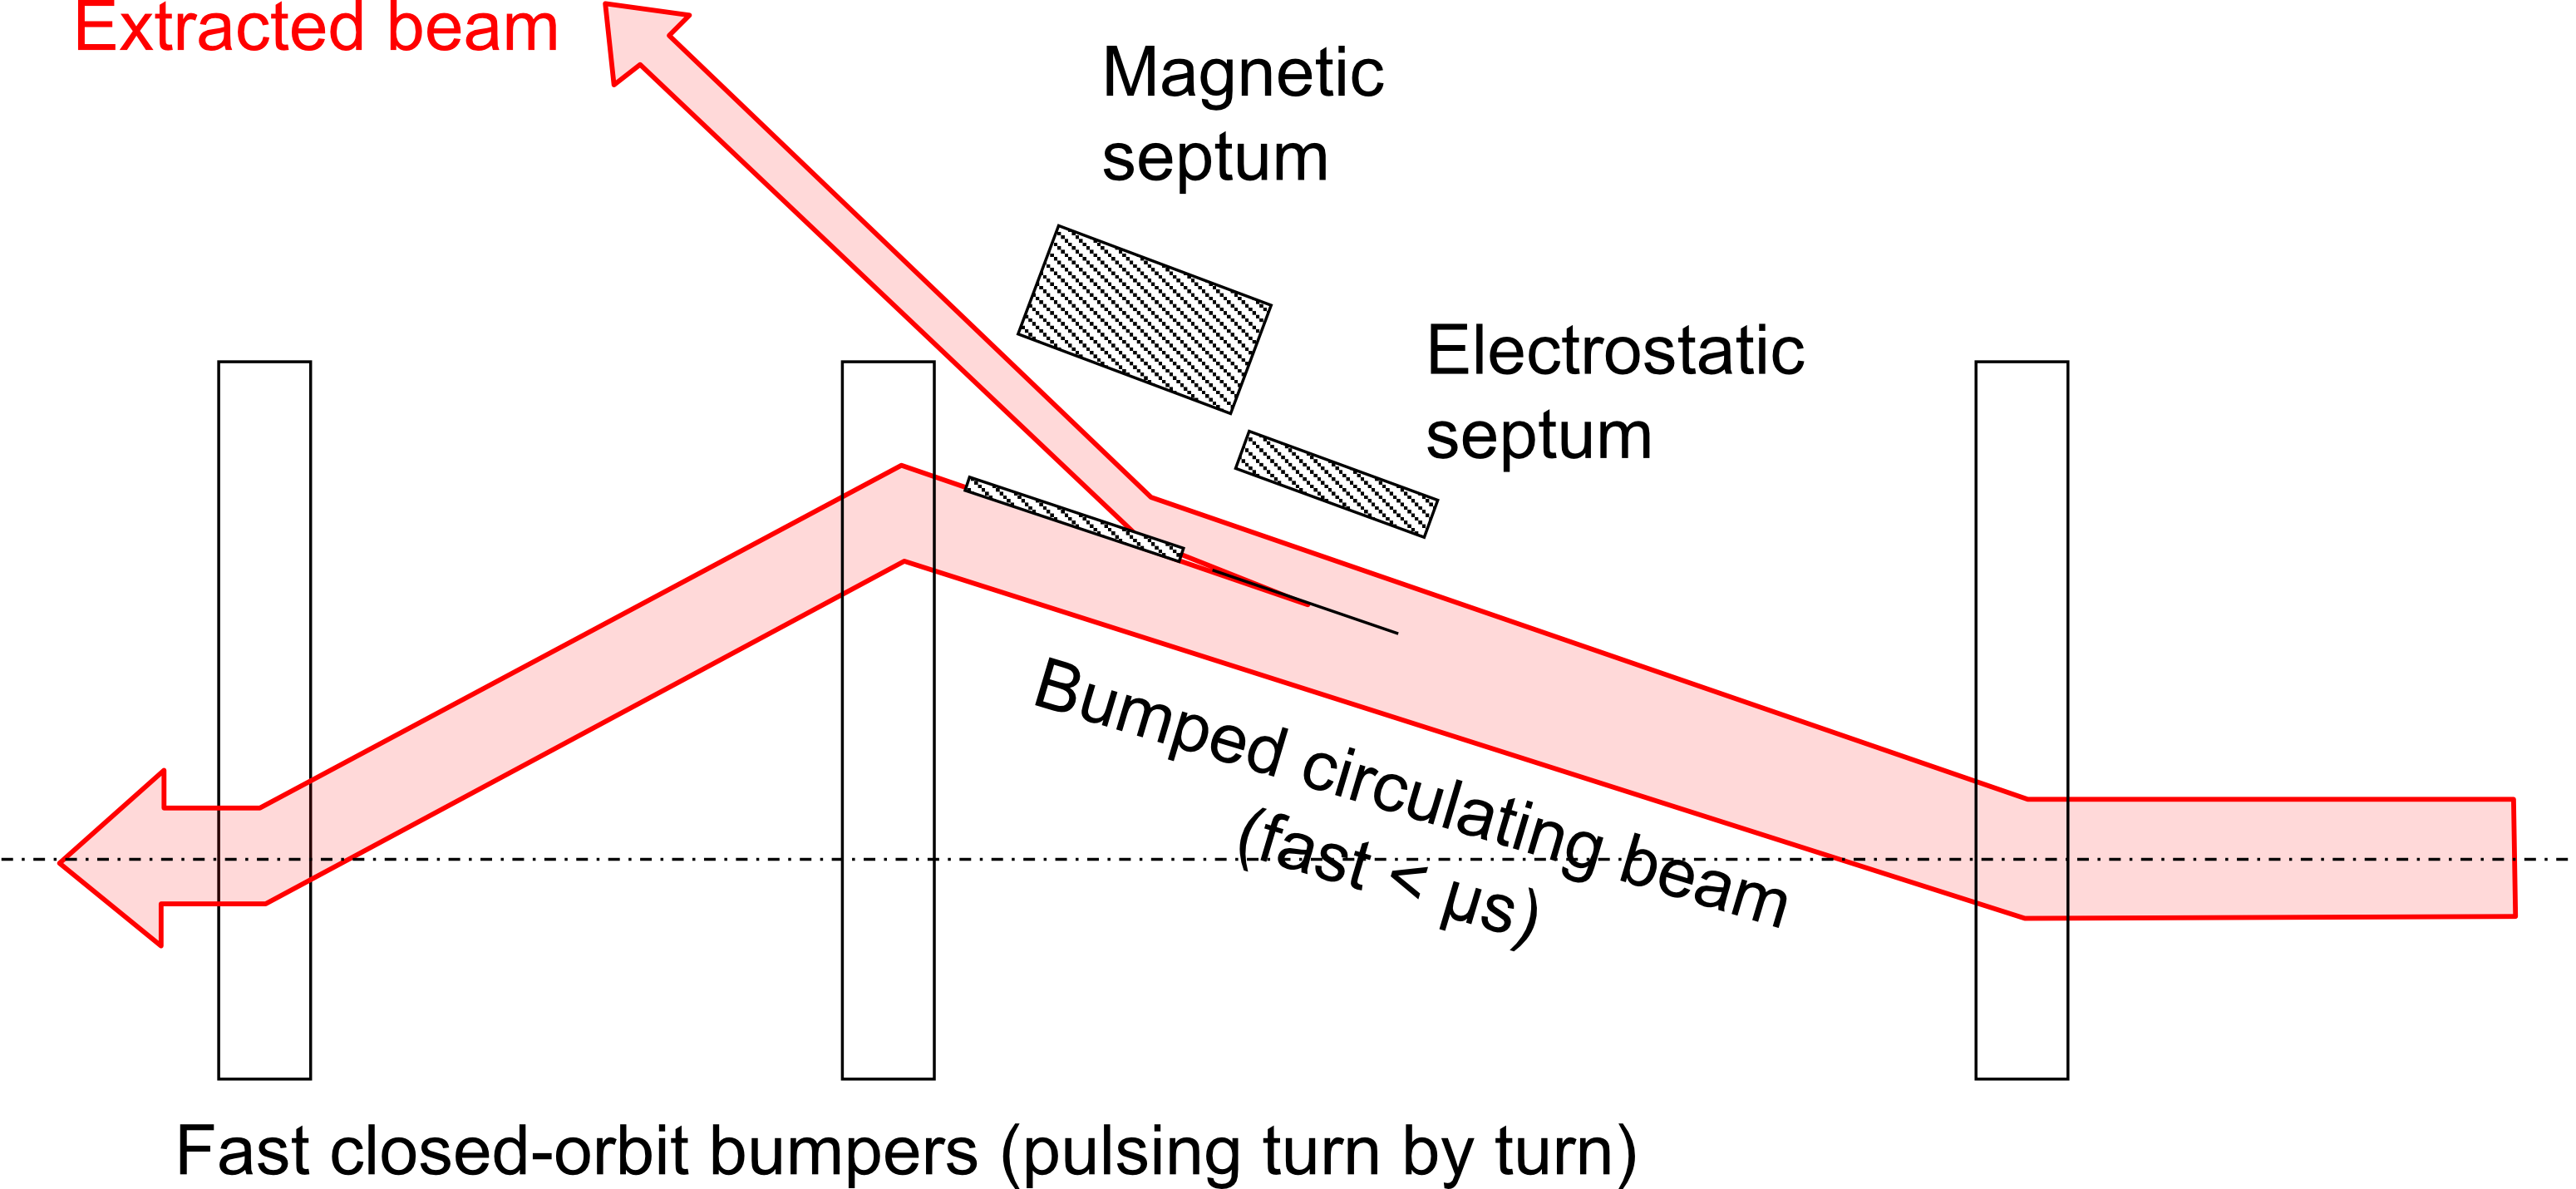
\includegraphics[width=\linewidth]{fastmulti.png}
  \caption{Diagram of a general multi-turn fast extraction system~\cite{Fraser:CAS}.}\label{fig:fast_multi_diagram}
\end{figure}

This method of increasing the spill time is, however, limited by the width of the septum blades. As the amount of beam scraped off per turn decreases, the effect of the particles lost on the septum blade increases. To maintain a reasonable extraction efficiency, the beam size would have to become exponentially large. For example, if a 50\% extraction efficiency is desired over $10^4$ turns, the beam thickness sliced off by the Electrostatic Septum (ES) must be the same as the thickness of the blade itself. For the SPS, the ES has an effective blade thickness of \qty{500}{\micro\meter}~\cite{sps-es.23.023501}. The required diameter of the beam, therefore, would be $2\cdot 25\mu m\cdot 10^4 = $ \qty{10}{\meter}~\cite{brunner}. This diameter would be larger than the beam pipes, and clearly physically impossible.

In order to provide spills over a longer duration, over many thousands of turns, \textit{slow extraction} must be used. 

\subsection{Introduction to Slow Extraction}

\textbf{Slow extraction} instead relies on exploiting resonance of the beam as it oscillates around the orbit of the machine. A full theoretical description of these effects will be detailed in \autoref{chap:theory}, but a brief explanation is offered here: the oscillatory motion of a beam can be controlled such that it returns to the same point along the accelerators circumference with the same oscillation phase, in order to be in harmonic resonance with the periodic field distribution of the ring. Great care is usually taken to avoid this effect in particle accelerators. However, with the correct configuration, this amplitude growth can be used alongside an ES to separate particles from their orbit, towards an MS, and into the extraction transfer line. Should the effect be slow enough, a small fraction of particles will reach the MS per turns.

The exploitation of resonance to induce extraction is by no means novel; a method akin to slow extraction was first proposed by J. Tuck and L. Teng in 1951~\cite{Couteur_1951}, and performed by Le Couteur at the Liverpool cyclotron in 1954~\cite{Couteur_1955}. Many such applications of slow extraction exist, using different effects to drive particles into resonance. This thesis will present some of these methods, particularly focussing on Radio-Frequency Knockout slow extraction.

Many medical synchrotrons, such as the MedAustron Synchrotron, use slow extraction to deliver beam to patients for ion beam cancer therapy~\cite{ArrutiaSota:2845862}, producing spills of up to \qty{30}{\second}\footnote{Limited to \qty{10}{\second} for patient treatment}. In human medical applications, safety is paramount. Therefore, the slow extraction process must be fully understood. Ripples in the intensity of beam have to be carefully controlled in order to provide a steady, predictable irradiation dose to patients.

Small medical synchrotrons are simpler\footnote{The PS contains 100 bending magnets along its circumference, as opposed to MedAustron's 16}, newer\footnote{The PS began operation in 1959, and is CERN's oldest accelerator still in operation. MedAustron was first certified in 2016.}, and have a far higher operational availability requirement than research accelerators such as the PS. At CERN's PS, however, that benefit cannot be relied upon. Machine time is in high demand, and studies are time-shared between machine development (MD), fixed-target experimental areas, LHC physics injection, and a wide array of other facilities. 

Simulations can therefore provide an important tool in understanding slow extraction spills. New methods can be rapidly developed and tested without requiring extensive (and expensive) machine studies, and wide parameter spaces can be explored to construct functional relationships between input parameters and spill output characteristics. 

\section{Modelling Slow Extraction}\label{sec:modelling-slow-extraction}

\Cref{sec:matrix} will introduce a mathematical model which can be used to numerically calculate particle trajectories in simple machines. However, with even the simplest of accelerators at CERN containing hundreds of components, computational models quickly become necessary. In addition, slow extraction can operate over many more accelerator turns than other processes, such as fast single-turn injection. In the PS, a spill length of \qty{0.5}{\second} would require approximate 230,000 turns. For even a reasonably powerful machine, these computational simulations quickly become time-consuming. 

To aid with the design and construction of CERN's Large Electron-Positron collider (LEP, the predecessor to LHC), the \textit{Methodical Accelerator Design Program} (MAD)~\cite{Iselin:MAD} was developed. This FORTRAN-based scripting tool allowed physicists to define the arrangement and strengths of magnetic elements around an accelerator (the \textit{lattice}), define beam parameters, and calculate the resulting motion of particles (the \textit{optics}). MAD, and its latest version, \verb|MAD-X|, quickly became the \textit{de facto} standard within CERN's beam physics community. However, in the twenty years since the release of \verb|MAD-X|, the landscape of computational accelerator physics has become awash with a wide array of tools, codes, and standards, each with their own specialisations. 

Newer tools are introducing improvements such as ``ready-to-go'' compatibility with General-Purpose Graphical Processing Unit (GPGPU) acceleration. GPUs are specialised hardware capable of performing highly optimised matrix and vector calculations. This makes them ideal for the matrix calculations required for particle accelerator simulations. Additionally, \textit{embarassingly parallel}\footnote{A problem which requires minimal to no effort to be separated into a large number of independent, concurrently-processed tasks.} tasks can be run on a large number of smaller processing platforms, rather than a single large platform. These platforms could be processing units within a GPGPU, or a discrete computer host on a batch-processing network.

\chapter{Accelerator Physics Theory}\label{chap:theory}

To construct accurate simulations of slow extraction methods, one must first understand the fundamental theory behind particle motion in a circular accelerator. This chapter will introduce the theory required to understand the motion of particles as they travel through an accelerator, and how such oscillatory motion can be exploited to perform slow extraction~\cite{Wiedemann}.
\section{Transverse Beam Dynamics}\label{sec:theory-transverse}

\subsection{Coordinate System}

The coordinate systems used to describe the dynamic motion of particles in an accelerator such as the PS relies on the periodic nature of a circular accelerator. Using a traditional Cartesian coordinate system would quickly introduce complications when describing circular trajectories, and so a local curvilinear coordinate system is used~\cite{BDSIM}.

The basis vectors for this system, $(\hat x, \hat y, \hat s)$, rotate in space as the reference particle moves along the accelerator. The longitudinal vector $\hat s$ is tangent to the reference particle's trajectory, and the $\hat x$ direction is parallel to the radius of the accelerator.  This system is shown in Figure~\ref{fig:frenet-serret}, along with the radius of the circular trajectory $\rho$, and the angle from the origin $s=0$. 

\begin{figure}[!h]
  \centering
  \includegraphics*[width=0.5\linewidth]{coordinate-system.png}
  \caption[Local coordinate system]{The vectors used to define the Frenet-Serret coordinate system.}\label{fig:frenet-serret}
\end{figure}

This coordinate system is known as a {\it Frenet-Serret} coordinate system, and can be rigorously defined by the unit vector {\it tangent} to the curve $\hat T$ (pointing in the direction of motion), the unit vector {\it normal} to the tangent and on the tangential plane $\hat N$, and the binormal unit vector $\hat B$, the cross product of $\hat T$ and $\hat N$. These unit vectors, forming an orthonormal basis spanning $\mathbb{R}^3$ are equal to the vectors $\hat x, \hat y, \hat s$ by:
\begin{equation}
\begin{pmatrix}\hat T\\\hat N\\\hat B \end{pmatrix}=\begin{pmatrix}\hat s\\-\hat x\\\hat y \end{pmatrix}
\end{equation}

The coordinate system $(\hat x, \hat y, \hat s)$ relies on the right-hand chirality (Figure~\ref{fig:rhr}) of the vector cross product for the $\hat x$ vector to point radially outwards from the centre of the machine, the $\hat y$ vector points upwards, and the $\hat s$ vector points in the direction of motion.

\begin{figure}[!h]
  \centering
  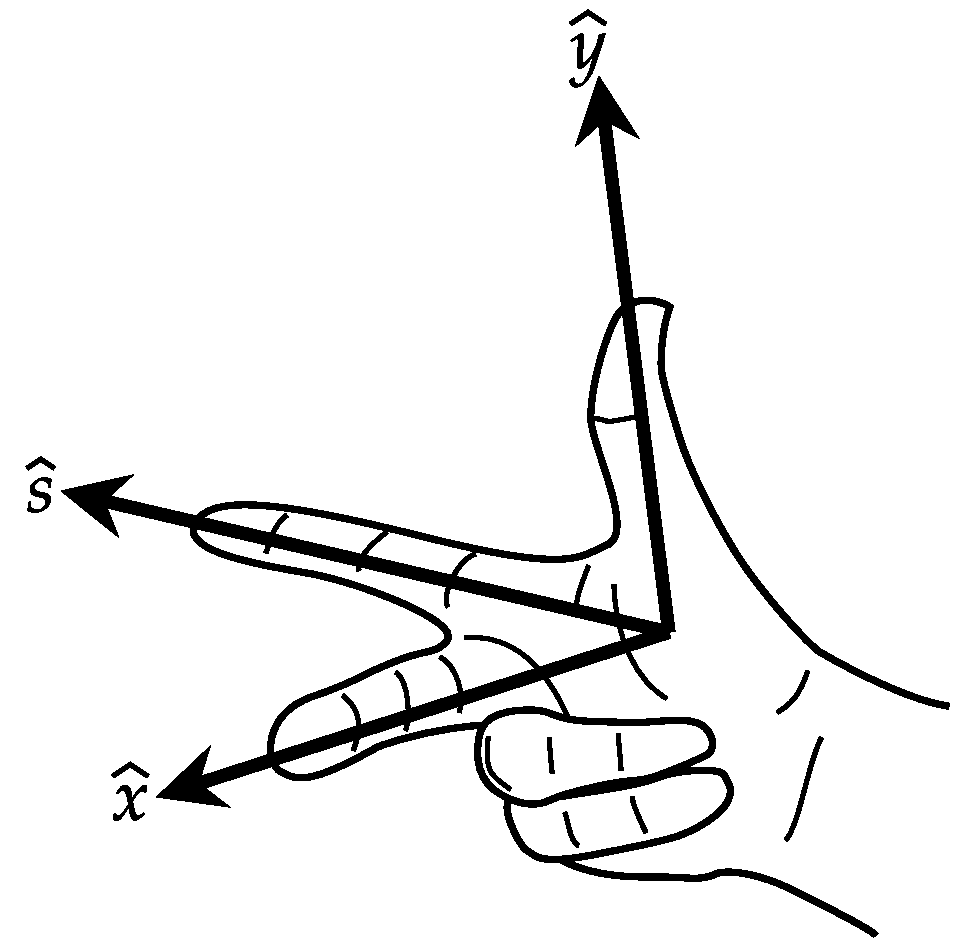
\includegraphics[scale=.25]{rhr.pdf}
  \caption[The right-hand rule]{The right-hand chirality rule defining the direction of $\hat x = \hat y \times \hat s$}\label{fig:rhr}
\end{figure}

\subsection{Special Relativity}

The equations of motion in this thesis consider particles moving at extremely high velocity, approaching the speed of light $c$. At CERN, before injection into the PS, particles are accelerated to \qty{2}{\giga\electronvolt}, and reach 94.8\% of the speed of light. At such speeds, relativistic effects are significant.

The Lorentz factor $\gamma$ is defined as the derivative of \textit{coordinate} time $t$ in the relativistic particle's reference frame, with respect to the \textit{proper} or \textit{lab} time $\tau$ in the observer's reference frame. It is calculated as:
\begin{equation}
    \gamma_c = \frac 1{\sqrt{1-\frac{v^2}{c^2}}}
\end{equation}
Also defined is the factor $\beta$
\begin{equation}
    \beta_c = \frac vc
\end{equation}
and the factor $\alpha$
\begin{equation}
    \alpha_c = \frac 1\gamma
\end{equation}

These factors will be referred to as $\alpha_c, \beta_c, \gamma_c$ to distinguish them from other parameters using $\alpha, \beta, \gamma$ (\autoref{subsec:trans_phase_space}).

One important distinction in a relativistic reference frame is the \textit{invariant} mass $m_0$ versus the \text{relativistic} mass $m$. The invariant mass, or \text{rest} mass of any object is the Newtonian mass measured in its own reference frame. From the \textit{lab} reference frame, this mass is measured as the relativistic mass, defined as:
\begin{equation}
    m=\gamma_c m_0
\end{equation}
This relativistic mass is conserved just the same as rest mass, and follows the $p=mv$ formula as in the rest frame. 
The rest \text{energy} $E_0$ and \textit{momentum} $m_0$ are likewise defined in the relativistic frame:
\begin{equation}
    E=\gamma_c m_0c^2
    \label{eq:relativistic_energy}
\end{equation}
\begin{equation}
    p=\gamma_c m_0v
    \label{eq:relativistic_momentum}
\end{equation}
For brevity, this report will always assume a relativistic frame, and all mentions of mass $m$, momentum $p$, or energy $E$ should be assumed to be relativistic unless otherwise stated.

\subsection{Particle Variables}

Following the basis vectors defining the coordinate system, the following variables are used to characterise the orbit of particles, dependent on $s$:

\noindent \textbf{In the transverse planes:}
\begin{itemize}
  \item $x(s)$ [m]~---~the particle's horizontal position with respect to the reference orbit.
  \item $y(s)$ [m]~---~the particle's vertical position with respect to the reference orbit.
  \item $x'(s)=\frac{dx}{ds}$ [rad]~---~the particle's horizontal angle with respect to the reference orbit.
  \item $y'(s)=\frac{dy}{ds}$ [rad]~---~the particle's vertical angle with respect to the reference orbit.
\end{itemize}
\textbf{In the longitudinal plane:}
\begin{itemize}
    \item $z=s-s_0$~---~the particle's longitudinal position with respect to the reference particle $s_0$.
    \item $\delta = \Delta p/p_0$~---~the particle's momentum difference with respect to the reference particle $p_0$.
    %\item $t(s)=-c\Delta t$ [m]~---~the particle's arrival delay with respect to the reference orbit, multiplied by the speed of light $c$.
    %\item $p_t(s)=\Delta E/pc$~---~the particle's energy difference, divided by the reference momentum times the speed of light $c$.
\end{itemize} 

These variables provide 6 vectors fully describing the position of a particle. However, for the remainder of this thesis, the pair of longitudinal variables $(z, \delta)$ will be treated separately to the transverse variable pairs $(x, x')$ and $(y, y')$. This enables a simpler understanding of the effects of beam bending and focussing magnets, as these effects are independent of the longitudinal variables.

\subsection{Design Orbit and Dipoles}

An understanding of particle dynamics in an accelerator can be built upon the Lorentz force, describing the force $\vec F$ acting on a charged particle with charge $q$ as it moves through an electric field $\vec E$ and magnetic field $\vec B$ with velocity $\vec v$, given as
\begin{equation}
\vec F_{\text{lorentz}} = q\cdot(\vec E+ \vec v\times\vec B)\label{eq:lorentz}
\end{equation}
This equation can already show why magnetic fields are typically used to bend particles along a circular trajectory and not electric fields; a particle with higher velocity $v$ will experience a greater force from a constant magnetic field $\vec B$, whereas the contribution from the electric field $\vec E$ will not benefit from the increasing velocity of a particle.

The other force experienced by a particle in an accelerator is a consequence of conservation of momentum:
\begin{equation}
\vec F_{\text{centrif.}}=\frac{m_0v^2}{\rho}\label{eq:centrifugal}
\end{equation} where $m_0$ is the particle's rest mass, and $\rho$ is the radius of the particle's orbit inside the accelerator.

Equating equations~\ref{eq:centrifugal} and~\ref{eq:lorentz} yields
\begin{equation}
B\rho=\frac pq
\label{eq:brho}
\end{equation}
The quantity $B\rho$ is known as the \textit{magnetic rigidity} of a beam, and defines the bending angle of a particle for a given magnetic field. 

If the relativistic momentum $p=mv$ of the particle is measured in \unit[per-mode = symbol]{\GeV\per\clight\per amu} (atomic mass unit), the magnetic rigidity can be expressed in Tesla-meters:
\begin{equation}
B\rho \left[\unit{\tesla\meter}\right] = 3.3356\cdot p\left[\unit{\giga\electronvolt\per\clight}\right]
\label{tesla-meters}
\end{equation} %B\rho\ \left[\unit{\tesla\meter}\right]=\frac pq=\frac AZ\times3.33564\times q\ \left[\unit[per-mode=symbol]{\GeV\per\clight\per\atomicmassunit}\right]
Referring again to~\autoref{eq:lorentz} (with the help of~\autoref{fig:rhr}), a magnetic field pointed vertically upwards (along the $\hat y$ vector) will cause a positively-charged particle with motion along the $\hat s$ vector to experience a bending force along the $-\hat x$ direction (illustrated in~\autoref{fig:dipole}). This formulation, however, only considers a single dipole. In reality, the bending magnet structure of accelerators typically consist of multiple dipoles placed around the ring, their power converters connecting in series. The arrangements of these bending magnets---referred to as Main Units (MU) in the context of the PS---will define the reference\footnote{Sometimes referred to as \textit{design} orbit} orbit in the accelerator.

\begin{figure}[h]
  \centering
  \includegraphics*[width=0.2\linewidth]{dipole-bending.png}
  \caption[Illustration of the force experienced by a charged particle in a magnetic dipole field.]{A ``front-on'' view of a dipole magnet, showing its magnetic field pointing down, and the Lorentz force experienced by a positively charged particle travelling into the page.}\label{fig:dipole}
\end{figure}

If $\alpha$ is the bending angle of a single MU, then $\alpha$ can be related to the magnetic rigidity by
\begin{equation}
\alpha=\frac{ds}\rho=\frac{B\ ds}{B\rho}
\end{equation}
Integrating this over all magnets in the ring, therefore, must be equal to one full revolution, $2\pi$. This provides one of the first key insights which is not obvious at first---that ``circular'' accelerators are in fact more complex shapes, with bending magnets at each vertex, and a \textit{drift} (accelerator sections without any significant electromagnetic field) or other non-bending multipole magnet at each side: in the case of the LHC, 1,232 dipole magnets are used to keep the beam on it's circular path; in the PS---100.

\subsection{Focussing and Multipoles}

While single-pair dipole magnets are used to bend the beam along the circular path, double-pair \textit{quadrupole} magnets are used to bound the transverse motion, and to prevent the beam from spreading (increasing in size) due to the intrinsic spread of position and angle. An arrangement of four magnetic poles creates a field stronger at higher $|x|$ displacement, causing particles to be pulled back towards the design orbit, ``focussing'' the beam in one transverse plane (while necessarily defocussing in the other). To correct for the defocussing in the other plane, a second quadrupole is placed further along in the beamline, with the magnetic poles arranged in the opposite orientation. This arrangement, known as a FODO lattice, is shown in \autoref{fig:quadrupole} (right).~\autoref{fig:sextupole} depicts a \textit{sextupole} magnet, with three pole pairs, which is used to correct for the dispersion effect of a dipole.

\begin{figure}
\centering
  \includegraphics*[width=0.9\linewidth]{fodo.png}
  \caption[Diagrams of a quadrupole magnetic field, and a FODO cell]{Diagram (left) showing the field of a \textit{normal} oriented quadrupole, providing focussing in $x$ but defocussing in $y$. The force experienced by a positively-charged particle is shown as dashed arrows. Right-hand diagram illustrates a FODO cell, where the structure of repeting focussing and defocussing quadrupoles can be related to the optical analogy of lenses.}\label{fig:quadrupole}
\end{figure}

\begin{figure}
    \centering
    \includegraphics*[width=0.4\linewidth]{sextupole.png}
    \caption{A diagram showing the field of a \textit{normal} oriented sextupole. The force experienced by a positively-charged particle is shown as dashed arrows.}\label{fig:sextupole}
\end{figure}

\subsection{Single-Particle Oscillatory Motion}

In a periodic (circular) accelerator, the linear equation for transverse motion takes the form of a differential equation:
\begin{equation}
  x''-x\cdot\left(k-\frac{1}{\rho^2}\right)=0
  \label{eq:diff_motion}
\end{equation} 
where $k$ is the normalised quadrupole coefficient, defined as
\begin{equation}
  k=\frac{q}{p}\cdot\frac{dB_y}{dx}
  \label{eq:quadrupole}
\end{equation}
The periodicity of circular accelerators requires that $k$ is also periodic, and the same gradient is seen after one turn. The $1/\rho^2$ term represents the effect of the dipole bending field, providing a weak focussing effect. If we enforce the periodicity\footnote{i.e. that the quadrupoles do not change between consecutive revolutions} in $s$ of $k$, Equation~\ref{eq:diff_motion} can be rewritten in a compact form
\begin{equation}
  x''(s)-\tilde{k}(s)x(s)=0
  \label{eq:hill}
\end{equation} where the quadrupole focussing component $\tilde{k}(s)$ is now a function of $s$. With the given periodic boundary condition $\tilde k(s+L)=\tilde{k}(s)$,~\ref{eq:hill} is known as the Hill's equation. 
Following Floquet's theorem~\cite{Rossbach:247501}, the general solution to this equation takes the form of
\begin{equation}
x(s) =\sqrt{\varepsilon}\sqrt{\beta(s)}\cos(\varphi(s)-\varphi_0)
\label{eq:motion_x}
\end{equation} 
where $\varphi(s)$ is the oscillation phase, $\varphi_0$ is the initial condition, and $\varepsilon$ is an integration constant. $\varphi_0$ and $\varepsilon$ are constants of a trajectory, and so the transverse oscillation of a particle is given by the special $\beta$ function. The $\beta$ function must also satisfy the periodic constraint $\beta(s+L)=\beta(s)$, and is related to the $\varphi$ phase function by the following equation:
\begin{eqnarray}
  \varphi(s) = \int^s_0\frac{ds'}{\beta(s')}
  \label{eq:phase_and_beta}
\end{eqnarray}

Taking the derivative of~\eqref{eq:motion_x} with respect to $s$ gives an equation for the angle of the trajectory:
\begin{equation}
x'(s)=\sqrt{\varepsilon}\sqrt{\beta(s)}\left(\frac12\beta'(s)\cos(\varphi(s)-\varphi_0)+\sin(\varphi(s))\right)
\label{eq:motion_px}
\end{equation}

The overall phase advance of transverse oscillations over one revolution of $2\pi$ is known as the \textit{betatron tune} of the accelerator, and is defined as
\begin{equation}
  Q=\frac1{2\pi}\oint\frac{ds}{\beta(s)}
  \label{eq:betatron_tune}
\end{equation}
This quantity, often simply referred to as \textit{tune}, effectively indicates how many complete transverse oscillations a particle makes in one turn. The fractional part of this value is the most significant, and the integer part of a referenced tune may sometimes be omitted.

Particles with momentum different to the reference particle $p_0$ will experience different focussing effects in quadrupoles. This slight change in focussing will effect the oscillatory motion of off-momentum particles, and result in a spread of tunes throughout a distribution of particles. The variation of this tune, with respect to the variation in momentum, is characterised by the \textit{normalised chromaticity} (where it is divided by $Q$), variously defined as $Q'$ or $\eta$:
\begin{equation}
  Q' = \frac{\Delta Q/Q}{\Delta p/p}
  \label{eq:chroma}
\end{equation}

\subsection{Phase Space}\label{subsec:trans_phase_space}

\autoref{eq:motion_x} and~\autoref{eq:motion_px} introduced an integration constant $\varepsilon$, which is a characteristic parameter of the particle or ensemble of particles. It is known as (transverse) emittance, and is usually considered with particle ensembles in mind. These two equations can be manipulated to provide an expression for $\varepsilon$:
\begin{equation}
  \varepsilon = \gamma(s)x^2(s)+2\alpha x(s)x'(s)+\beta(s)x'^2(s)
  \label{eq:emittance}
\end{equation} where 
\begin{equation}
  \alpha(s) = -\frac12\frac{d\beta(s)}{ds}
  \label{eq:alpha}
\end{equation} and
\begin{eqnarray}
  \gamma(s) = \frac{1+\alpha^2(s)}{\beta(s)}
  \label{eq:gamma}
\end{eqnarray}
These two values, along with $\beta$, form the \textit{Courant-Snyder Parameters}~\cite{courantsnyder}, commonly referred to as the \textit{twiss} parameters\footnote{Even Richard Q. Twiss, a British astronomer, was himself unsure as to how the parameters became attributed to him~\cite{richardtwiss}.}. 

These parameters can be readily understood in the \textit{phase space} of $(x, x')$. Illustrated in~\autoref{fig:twiss-phase-space}, \autoref{eq:emittance} describes an ellipse, which covers the area of the particle ensemble in phase space, the area of which is given by $\pi\cdot\varepsilon$. 

\begin{figure}[h]
  \centering
  \includegraphics*[width=0.6\linewidth]{phase-space-with-twiss.png}
  \caption{A phase space ellipse in $(x, x')$ and its relation to the Twiss parameters.}
  \label{fig:twiss-phase-space}
\end{figure}

Liouville's theorem states that, under conservative forces and at fixed energy, this emittance is conserved\footnote{\textit{Normalised} emittance is conserved during acceleration where energy is not fixed}, and no external field can change it. Hence,~\autoref{eq:motion_x} provides it as an invariant of motion. 

\subsection{Dispersion}\label{sec:transdisp}

We now consider the oscillatory motion of \textit{multiple} multi-energetic beams, with reference to the ideal particle. This ideal particle, with reference momentum $p_0$ and initial conditions all equating to zero, has a path through the field centre of all quadrupoles, and so experiences no quadrupole effect $k$. This means that its motion is controlled by the weak dipole focussing $1/\rho^2$. A nominal particle, still with momentum $p_0$ but with initial displacement and/or angle conditions, will perform closed-loop betatron oscillations around this path. 

A particle with a momentum offset, $\Delta p = p-p_0$, will still satisfy~\ref{eq:diff_motion} from before, but in the inhomogeneous form
\begin{equation}
  x''(s)-x\left(k-\frac 1{\rho^2}\right)=\frac 1\rho\frac{\Delta p}{p_0}
\end{equation}
We can use the homogeneous solution previously found to form the complete solution $x(s)=x_h(s)+x_i(s)$. This inhomogeneous term $x_i(s)$, is normalised by the momentum difference to produce the Dispersion function
\begin{equation}
  D(s)=\frac{x_i(s)}{\nicefrac{\Delta p}{p_0}}
  \label{eq:dispersion}
\end{equation} describing how the additional amplitude of an off-momentum particle depends on the momentum difference. 
This dispersion function satisfies, for the circumference of the machine:
\begin{equation}
  D''-D\left(x-\frac1{\rho^2}\right)=\frac 1{\rho(s)}
\end{equation}

\subsection{Matrix Formalism}\label{sec:matrix}

\autoref{eq:motion_x} and \autoref{eq:motion_px} can be solved by imposing initial conditions $x_0$ and $x'_0$ instead of periodic boundary conditions:
\begin{equation}
  x(s)=x_0\cos\left(\sqrt{K}\cdot s\right)+\frac{x'_0}{\sqrt{K}}\sin\left(\sqrt{K}\cdot s\right)
\end{equation}
\begin{equation}
  x'(s)=-x_0\sqrt{K}\sin\left(\sqrt{K}\cdot s\right)+x'_0\cos\left(\sqrt{K}\cdot s\right)
\end{equation}
where $K$ now combines the quadrupole focussing effect $k$ (\autoref{eq:quadrupole}) and the dipole weak focussing effect:
\begin{eqnarray}
  K=\frac1{\rho^2}-k
\end{eqnarray}

These two equations can be written as a matrix equation:
\begin{equation}
  \begin{pmatrix}
    x \\
    x'
  \end{pmatrix}
  =
  \bf{M}
  \begin{pmatrix}
    x_0 \\
    x'_0
  \end{pmatrix}
\end{equation}
where $\bf{M}$ is the transfer matrix
\begin{equation}
  \bf{M}=
  \begin{pmatrix}
    \cos\left(\sqrt{K}\cdot s\right) & \frac1{\sqrt{K}}\sin\left(\sqrt{K}\cdot s\right) \\
    -\sqrt{K}\sin\left(\sqrt{K}\cdot s\right) & \cos\left(\sqrt{K}\cdot s\right)
  \end{pmatrix}
\end{equation}

The definition of this transfer matrix $\bf M$ can be expanded to define the variety of magnets used in an accelerator. In the simple case, where no magnet is present, we define the transfer matrix for a drift space of length $L$:
\begin{equation}
  \bf{M}_{drift,x}=\bf{M}_{drift,y}=
  \begin{pmatrix}
    1 & L \\
    0 & 1
  \end{pmatrix}
\end{equation}

For a normal dipole magnet bending only horizontally, where $k=0$ and $K_x=1/\rho^2$, the transfer matrix is:
\begin{equation}
  \bf{M}_{dipole,x}=
  \begin{pmatrix}
    \cos\left(\frac L\rho\right) & \rho\sin\left(\frac L\rho\right) \\
    -\frac{\sin\left(\frac L\rho\right)}{\rho} & \cos\left(\frac L\rho\right)
  \end{pmatrix}
\end{equation}
\begin{equation}
  \bf{M}_{dipole,y}=\bf{M}_{drift,y}
\end{equation}

Further matrix equations can be defined for other magnets. If we define the properties of each element in the accelerator (the lattice), we can then define the transfer matrix for the entire accelerator as the product of the transfer matrices of each element. For example, a FODO lattice with an initial bending dipole can be defined as:
\begin{equation}
  \bf{M}_{total} = \bf{M}_{dipole} + \bf{M}_{quad} + \bf{M}_{drift} - \bf{M}_{quad} + \bf{M}_{drift} +\cdots
\end{equation}

This is the principle by which \textit{particle tracking codes}, such as \verb|MAD-X|, operate. An input lattice file defines the structure and properties of the magnets composing the accelerator, and particle variables are then computed with matrix multiplication. 

Expanding on the idea of matrix formalism and the phase space ellipse, many particle tracking codes operate in \textit{normalised} phase space $(x_n, x'_n)$---that is, where the phase space of $(x, x')$ is linearly transformed in a way which results in the phase space ellipse becoming circular. The matrix transformation is therefore defined as
\begin{equation}
  \begin{pmatrix}
    x_n \\
    x'_n
  \end{pmatrix} = 
  \begin{pmatrix}
    \frac{1}{\sqrt{\beta_x}} & 0 \\
    \frac{\alpha_x}{\sqrt{\beta_x}} & \sqrt{\beta_x}
  \end{pmatrix} \begin{pmatrix}
    x \\
    x'
  \end{pmatrix}
  \label{eq:normalised}
\end{equation}

\section{Longitudinal Dynamics}\label{sec:long}

Where the transverse planes principally consider bending and focussing effects from magnetic fields, the longitudinal plane considers acceleration effects from RF fields. Returning again to~\autoref{eq:lorentz}, we instead now consider the \textit{electric} component:
\begin{equation}
  \vec F = q\vec E = \frac{dp}{dt}
\end{equation} 
An electric field of magnitude $E_0$ travelling in the $s$ direction can be defined as
\begin{equation}
  E_s = E_0\cos(\omega_{RF}t)
\end{equation} where $\omega_{RF}$ is the RF frequency. Therefore, for a synchronous particle with synchronous phase $\phi_s$, the rate of energy gain is
\begin{equation}
  \frac{dE_s}{ds}=eE_0\sin\phi_s
\end{equation}

In a synchrotron, where the orbit of particles is of constant radius, the magnetic field $B$ needs to increase in time (\textit{ramp}) as the particle is accelerated. Additionally, to keep the particle in phase with the RF cavity, the frequency of the RF $\omega_{RF}$ must follow the particle's energy gain. This synchronous condition, for velocities $v\ll c$, is defined as
\begin{equation}
  \frac{2\pi\rho}{v_s}=\frac h{\omega_{RF}}
\end{equation} where $v_s$ is the synchronous particle velocity and $h$ is the RF harmonic, the number of RF cycles per revolution. For East Area beams in the PS, $h=8$ acceleration is used. This means that there are eight stable ``particles'', spread equidistantly around the ring circumference. 

To keep a particle with increasing energy bent along a path of constant radius, the magnetic field $B$ of the bending dipoles must increase as RF acceleration occurs. Recalling~\autoref{eq:brho}, and deriving by time, obtains
\begin{equation}
  \frac{dp}{dt} = q\rho\dot B
\end{equation}
For one turn in a synchrotron, this results in a momentum gain
\begin{equation}
  \Delta p_{rev} = q\rho\dot B T_{rev}=\frac{Lq\rho~R\dot B}v
\end{equation} where $L$ is the machine length. 
The energy gain $\Delta E=v\Delta p$ per revolution is therefore
\begin{equation}
  \Delta E_{rev} = Lq\rho~R\dot B=qV\sin \phi_s
  \label{eq:ef_sin}
\end{equation} where $\phi_s$ is the synchronous phase. This stable phase therefore changes while energy is ramped:
\begin{equation}
  \phi_s=\arcsin\left(L\rho\frac{\dot B}{V_{RF}}\right)
  \label{eq:sync_phase}
\end{equation}

\subsection{Dispersion}

Next, akin to~\autoref{sec:transdisp}, we consider small perturbations in momentum with respect to an ideal path. We define two parameters:
\begin{equation}
  \alpha_p = \frac{\Delta L/L}{\Delta p/p}
\end{equation} where $\alpha_p$, the \textit{momentum compaction factor}, is distinct from the relativistic $\alpha_c$ and Twiss parameter $\alpha$.
\begin{equation}
  \eta = \frac{\Delta f_{rev}/f_{rev}}{\Delta p/p}
  \label{eq:slip_factor}
\end{equation} where $\eta$, the \textit{slip factor}, is the relative change of revolution frequency with momentum.

Using the dispersion function~\autoref{eq:dispersion}, we can relate the momentum compaction factor to its effect on orbit length $s_0$~\cite[5.1]{lbd:tecker}
\begin{equation}
  \alpha_p=\frac 1L\int\frac{D_x(s)}{\rho(s)}\ ds_0
\end{equation}

Using the revolution frequency\footnote{NB: $\beta_c$ here refers to the relativistic Lorentz factor $v/c$ } $f_{rev}=\beta_c c/2\pi R$, we define the relative revolution frequency change $\Delta f_{rev}$ as
\begin{equation}
  \Delta f_{rev} = \frac{d\beta_c}{\beta_c}-\frac{dR}R=\frac{d\beta_c}{\beta_c}-\alpha_p\frac{dp}p
\end{equation} 



This defines a \textit{transition energy} $\gamma_{tr}$ such that $\eta=0$, causing no change in revolution frequency $f_{rev}$ for a small momentum change $\Delta p$:
\begin{equation}
  \gamma_{tr}=\frac 1{\sqrt{\alpha_p}}
\end{equation}
\textit{Above} this transition energy, where $\eta<0$, the particle has velocity $v\rightarrow c$, and so the path-length change dominates the velocity change. This is the standard configuration of accelerators.
\textit{Below} this transition energy, where $\eta >0$, the increase of velocity is significantly larger than the path-length change effect.
\textit{At} this transition energy, both effects compensate, and so $f_{rev}$ becomes independent of $\Delta p$. Here, the \textit{synchrotron} longitudinal oscillations stop, and particles not on the synchronous phase $\phi_s$ will rapidly gain energy, and become lost due to dispersion $D$.


\subsection{Longitudinal Phase Space}\label{sec:long_phase_space}

These effects can be analysed by considering phase space coordinates---this time in the longitudinal plane. This space is constructed with variables $(\phi , \Delta p/p)$, and shown in~\autoref{fig:long_phase_space}. A full derivation for the longitudinal motion invariants can be found in~\cite{lbd:tecker}, where the synchronous phase $\phi_s$ defines the orbit with zero longitudinal (synchrotron) oscillation. Outside of the stable envelope, demarcated by the \textit{separatrix}, particles are lost to instability. The region within the separatrix is known as the \textit{RF bucket}, and the area occupied by stable particles, the \textit{RF emittance}.

\begin{figure}[h]
  \centering
  \includegraphics*[width=0.9\linewidth]{long-phase-space.png}
  \caption{Longitudinal Phase Space, showing particles at the synchronous phase $\phi_s$, inside stability, and in unstable motion. The separatrix, bold, separates these two regions.}\label{fig:long_phase_space}
\end{figure}

\section{Slow Extraction}\label{sx}
Now that the fundamentals of accelerator beam physics are established, this section will introduce the principles behind \textit{slow extraction} (SX). Various methods of performing SX will be covered, but the particular method covered in this thesis---\textit{Radio-Frequency Knockout} (RFKO)---will be described in detail.

\subsection{Sextupoles and $\nicefrac 13$-Integer Resonance}

\Cref{sec:transdisp} introduced the concept of dispersion in reference to a multi-energetic beam. These effects are controlled with the use of sextupole magnets. The transverse field of a sextupole magnet has the form
\begin{equation}
  B_x = -6B_3xy
\end{equation}
\begin{equation}
  B_y = -3B_3(x^2-y^2)
\end{equation} where
\begin{equation}
  B_3=-\frac 16\left(\frac{d^2B_y}{dx^2}\right)_0
\end{equation}

In \textit{normalised} coordinates (\autoref{eq:normalised}), these effect of these fields (in a thin-lens approximation) becomes
\begin{align*}
  \Delta x_n&=0 & \Delta x_n'&=S(x^2-\frac{\beta_y}{\beta_x}y^2) \\
  \Delta y_n&=0 & \Delta y_n'&=-2S\frac{\beta_y}{\beta_x}xy
\end{align*}
where $S$, the normalised sextupole strength, is
\begin{equation}
  S=\frac 12\beta_x^{\nicefrac 23}l_sk'
  \label{eq:normalised_sextupole_strength}
\end{equation} where $l_s$ is the sextupole equivalent length, and $k'$ is the normalised sexutpole field:
\begin{equation}
  k'=-6\frac{B_3}{B\rho}
\end{equation}
For extraction driven in the horizontal transverse plane, the dynamics of the vertical transverse plane are neglected as these remain independent. Recalling the matrix formalism established in~\autoref{sec:matrix}, we use a general transfer matrix for $n$ turns with a betatron tune $Q$:
\begin{equation}
  \bf M_n=
  \begin{pmatrix}
    \cos(2\pi nQ_x)  & \sin(2\pi nQ_x) \\
    -\sin(2\pi nQ_x) & \cos(2\pi nQ_x)
  \end{pmatrix}
\end{equation}
The tune of a particle is then defined as a third-integer, i.e.
\begin{equation}
  Q_x=i\pm\nicefrac 13 +\delta Q,\ i\in\mathbb{Z}, |\delta Q|\ll\nicefrac 13
\end{equation} 
The tune distance, $\delta Q$, is therefore the distance of the particle from the resonance. The $n$-turn matrix can then be approximated for \textit{modulo}-3 turns:
\begin{equation}
  \begin{pmatrix}
    x\\x'
  \end{pmatrix}_1=
  \begin{pmatrix}
    -1/2 & \pm\sqrt{3}/2 \\
    \mp\sqrt{3}/2 & -1/2
  \end{pmatrix}\begin{pmatrix}
    x\\x'
  \end{pmatrix}_0
\end{equation}
\begin{equation}
  \begin{pmatrix}
    x\\x'
  \end{pmatrix}_2=
  \begin{pmatrix}
    -1/2 & \mp\sqrt{3}/2 \\
    \pm\sqrt{3}/2 & -1/2
  \end{pmatrix}\begin{pmatrix}
    x\\x'
  \end{pmatrix}_0
\end{equation}
\begin{equation}
  \begin{pmatrix}
    x\\x'
  \end{pmatrix}_3=
  \begin{pmatrix}
    1 & 6\pi\cdot\delta Q \\
    -6\pi\cdot\delta Q & 1
  \end{pmatrix}\begin{pmatrix}
    x\\x'
  \end{pmatrix}_0
\end{equation}
Therefore, a particle with $\delta Q=0$, i.e.\ exactly on resonance, will return to its original position after three turns. For such a particle, the change in position $x$ and divergence $x'$ from initial conditions $(x_0, x'_0)$ after three turns is therefore calculated as
\begin{equation}
  \Delta x_3 = {\varepsilon_Q} x'_0 + \frac 23 S x_0x'_0
  \label{eq:spiral_step}
\end{equation}
\begin{equation}
  \Delta x'_3 = -{\varepsilon_Q} x_0 + \frac 34 S (x_0^2-x'^2_0)
  \label{eq:spiral_kick}
\end{equation}
where ${\varepsilon_Q}$, the \textit{modified tune distance}, is defined as ${\varepsilon_Q} = 6\pi\cdot\delta Q$, and $S$ is the normalised sextupole strength (\autoref{eq:normalised_sextupole_strength}).

The values of $\Delta x_3$ and $\Delta x'_3$ are known as the \textit{spiral step} and \textit{spiral kick}.
The \textit{Hamiltonian} is now used to analyse this motion in phase-space. The Hamiltonian, $\bf H$ is a time-independent constant of motion, the contours of which describe the \textit{phase-space map}, the motion of a particle in normalised phase-space. Assuming the 3-turn time is small enough to be continuous, the \textit{Kobayashi Hamiltonian}~\cite{kobayashi} is defined as
\begin{equation}
  \textbf{H} =\frac{\varepsilon_Q} 2(x^2+x'^2)+\frac S4(3xx'^2-x^3)
\end{equation}

\begin{figure}
  \centering
  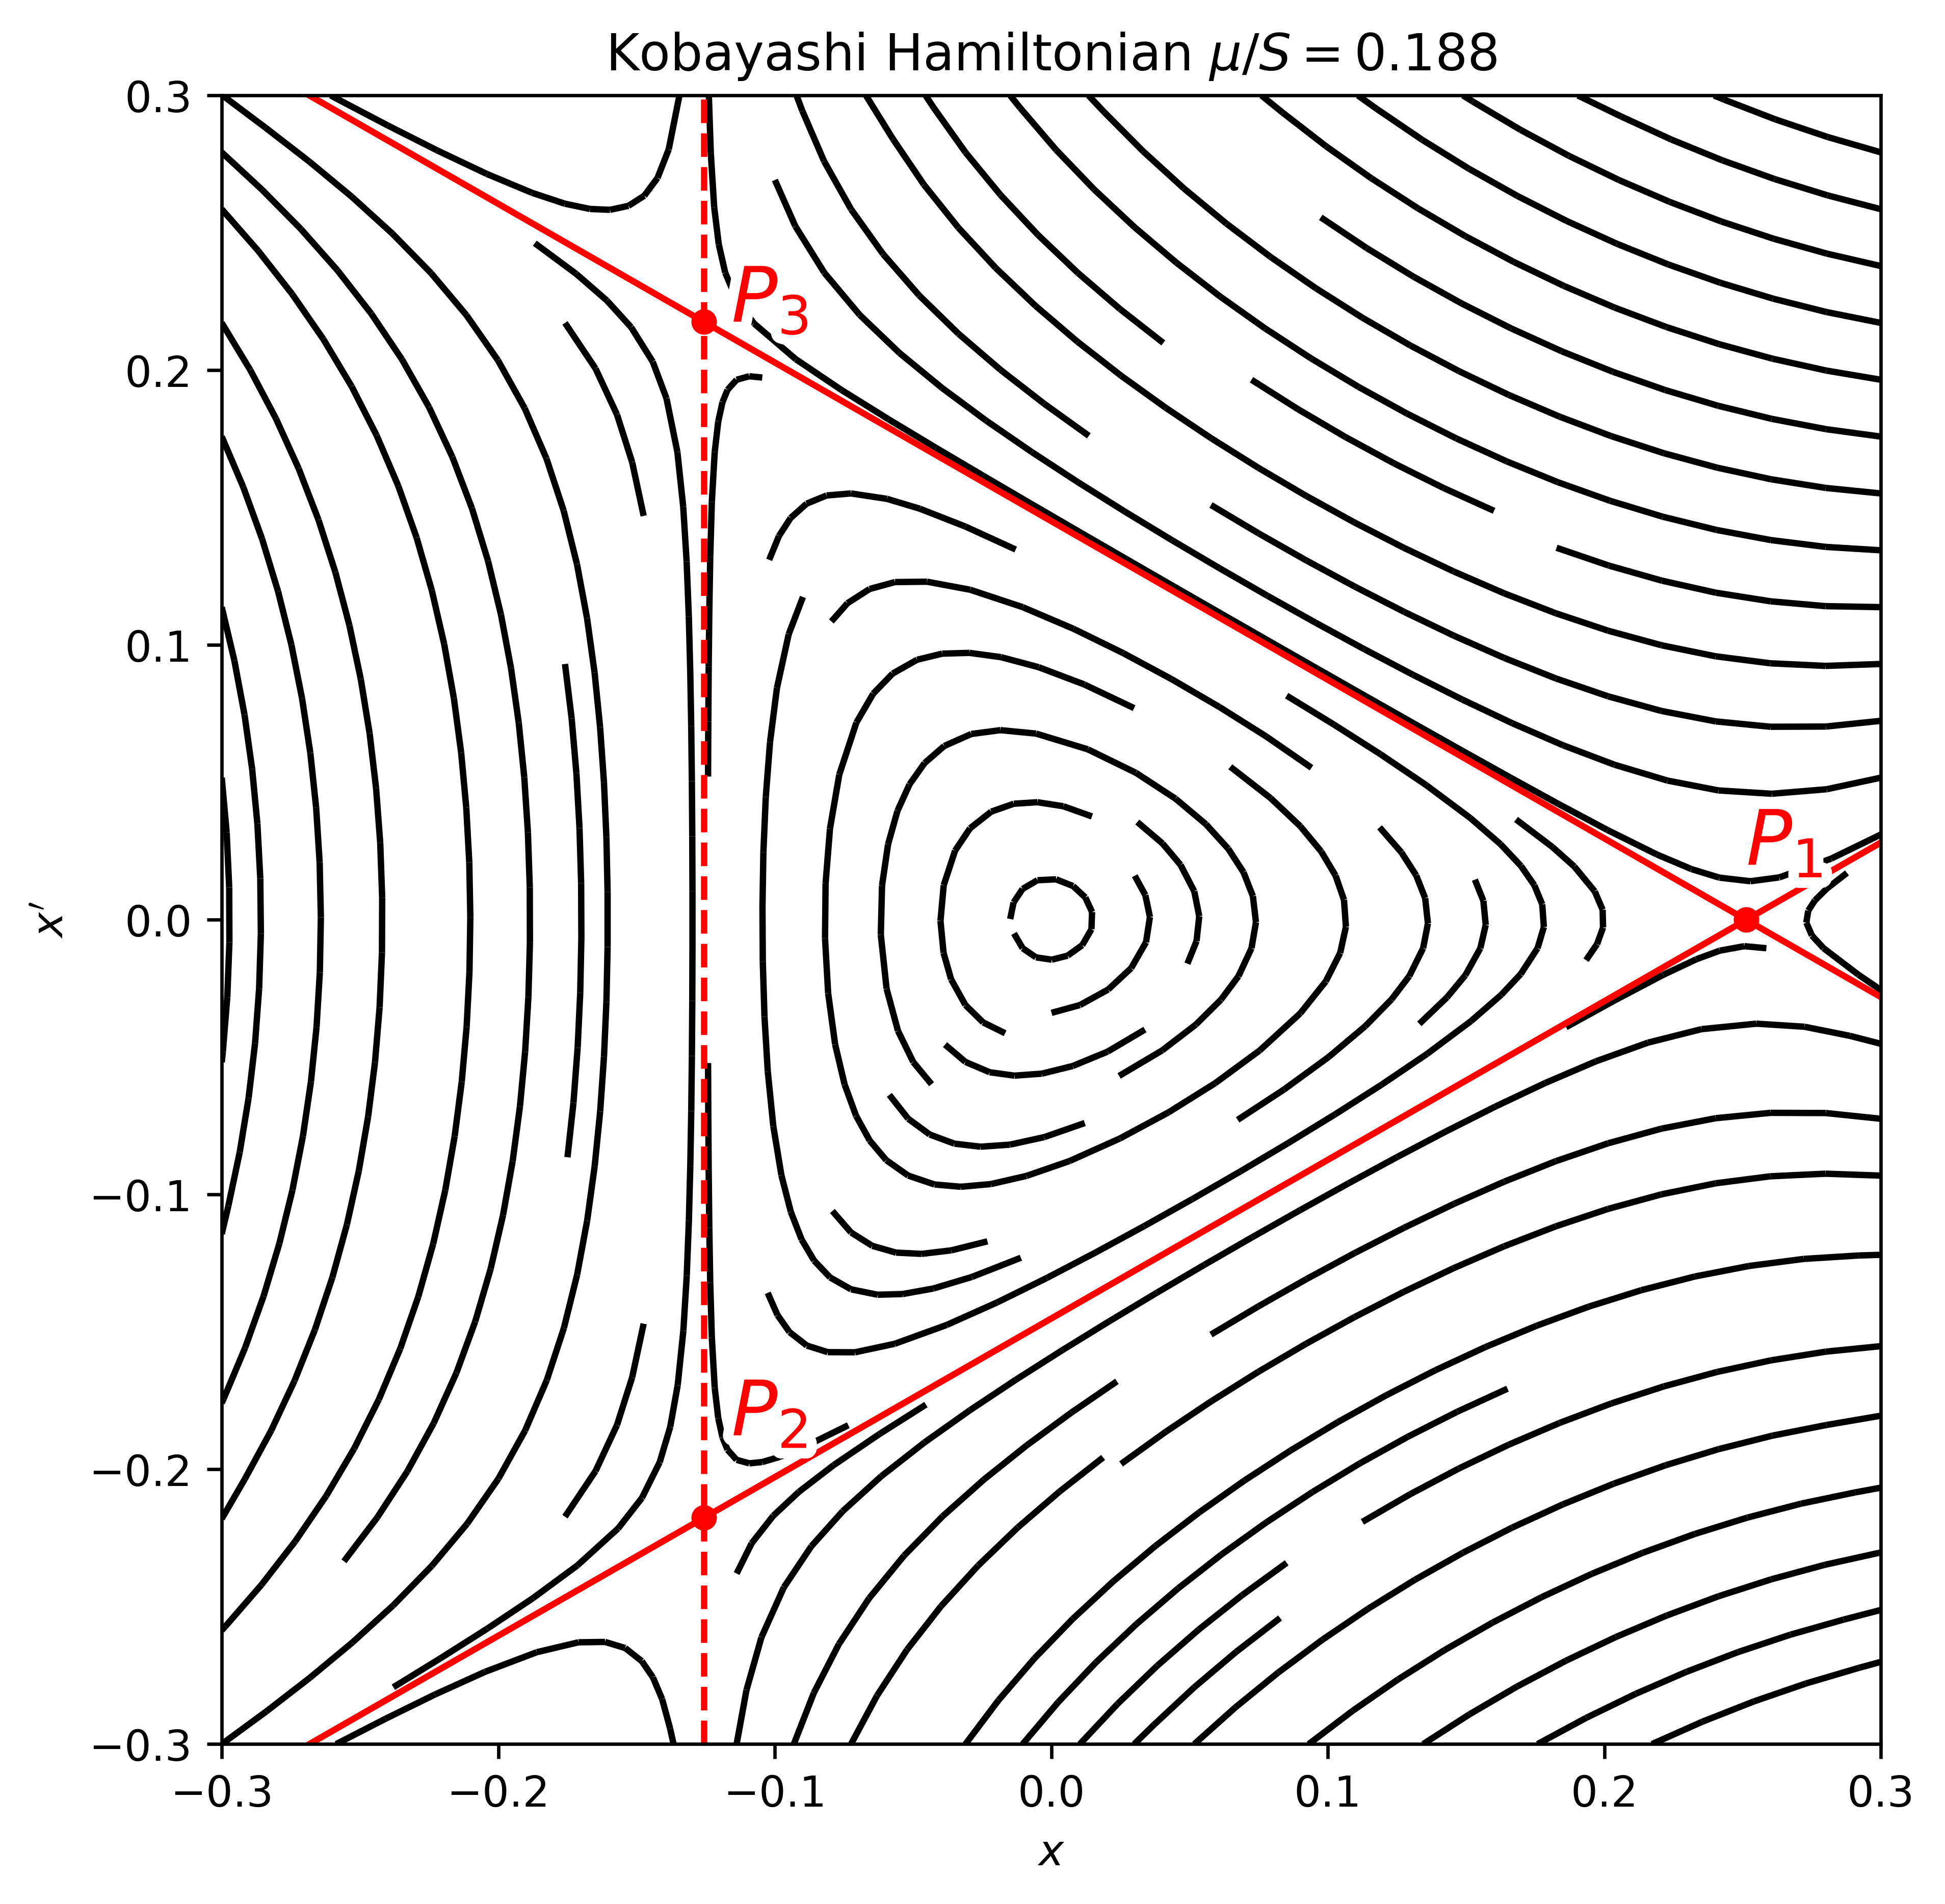
\includegraphics[width=0.6\linewidth]{kobayashi.png}
  \caption{Normalised phase-space map of the Kobayashi Hamiltonian, for a ratio ${\varepsilon_Q}/S=0.188$. The points $P_1, P_2, P_3$ are shown, with connecting lines.}\label{fig:kobayashi}
\end{figure}

The first term describes the typical circular phase-space motion familiar from~\autoref{subsec:trans_phase_space}, with a sextupole strength $S=0$ (i.e. a linear machine). The second term describes the sextupole effect, transforming the elliptical map into a triangular trajectory for increasing values of $x$ and $x'$. The phase-space map is shown in~\autoref{fig:kobayashi}. A boundary triangle is easily identified from the map, which defines the trajectory of the stable particle with greatest possible amplitude, before the motion becomes unstable. Outside of this stable region, the particle trajectories do not close on themselves, and the particle will rapidly gain amplitude. The region bounded by this \textit{separatrix} is known as the \textit{acceptance} the size of which is defined by $|{\varepsilon_Q} /S|$, and can be found by factorising $\bf H$ at at a value of $(2{\varepsilon_Q} /3)^3/S^2$, which factorisses to three points:
\begin{eqnarray}
  P_1 &=& \left(\frac 43 \frac{\varepsilon_Q} S,    0                       \right) \\
  P_2 &=& \left(-\frac 23 \frac {\varepsilon_Q} S,  -\frac{2{\varepsilon_Q}}{\sqrt 3 S} \right) \\
  P_3 &=& \left(-\frac 23 \frac {\varepsilon_Q} S,  \frac{2{\varepsilon_Q}}{\sqrt 3 S} \right)
\end{eqnarray}
The $x$ location of the stable particle, $h$ can also be defined as
\begin{equation}
  h=\frac 23 \frac {\varepsilon_Q} S = \frac{4\pi}S\delta Q
  \label{eq:apothem}
\end{equation}
Therefore, the lines connecting $P_1, P_2$ and $P_1, P_3$ (solid lines in \autoref{fig:kobayashi}), along with the vertical line at $-h$ (dashed line in \autoref{fig:kobayashi}), define the separatrix. The acceptance, the area bounded by the separatrices, is defined as $A=3\sqrt 4 h^2$.

\subsection{Slow Extraction Principles}
The fundamental principle of slow extraction exploits the unstable boundary created by sextupolar fields. After a beam is injected and stable, this \textit{waiting} beam is accelerated towards the $\nicefrac 13$-integer resonance. A particle at resonance will then ``lock on'' to one of the separatrix arms, and its amplitude will grow in steps of three turns, rotating around the three separatrices. By carefully controlling the rate at which particles enter resonance, the 3-turn amplitude growth (spiral step) can be adjusted to create a desired flux of particles entering resonance. After a number of turns of amplitude growth (typically hundreds), an electrostatic septum located at some distance from the waiting beam will provide a kick necessary to extract the particles. A real-world diagram of slow extraction is shown in~\autoref{fig:real-world}.

\begin{figure}
  \centering
  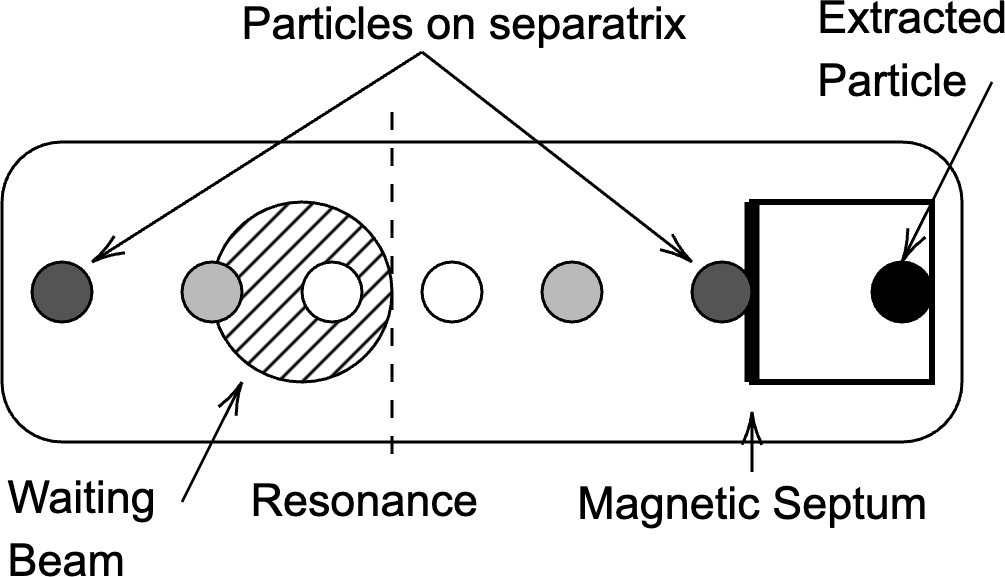
\includegraphics[width=0.6\linewidth]{real-world.png}
  \caption{A real-space diagram of momentum-driven slow extraction, looking along the $s$ direction at the magnetic septum location. The waiting beam approaches resonance (dashed), and some particles begin large turn-by-turn oscillations (increasing shaded gradient with turn number) before they jump the septum blade (thick black line) and will be extracted.}\label{fig:real-world}
\end{figure}

There are a variety of methods to provide acceleration of the beam towards resonance, which fall into two categories. \textit{Momentum-driven} methods rely on accelerating the beam towards a stationary resonance by controlling the momentum $\Delta p/p$. \textit{Amplitude-driven} methods, however, use transverse noise or RF excitation at the beam's revolution frequency to create increasing betatron amplitudes. 

Other methods involve moving the resonance itself, by changing the tune of the machine. This can be accomplished by using dipoles, quadrupoles, or sextupoles, but is susceptible to complications arising from the changing transverse optics. Implementations would require active compensation to maintain the beam's position, size, and ultimately, stability.% Quadrupole-driven extraction is, additionally, highly sensitive to power-supply ripples---residual variation in the voltage/current produced by AC-DC power converters. 

These various categories are not mutually exclusive, and some of the methods discussed will use a combination of effects to achieve slow extraction.

\subsection{Steinbach Diagram}\label{sec:steinbach}

\begin{figure}[ht]
  \centering
  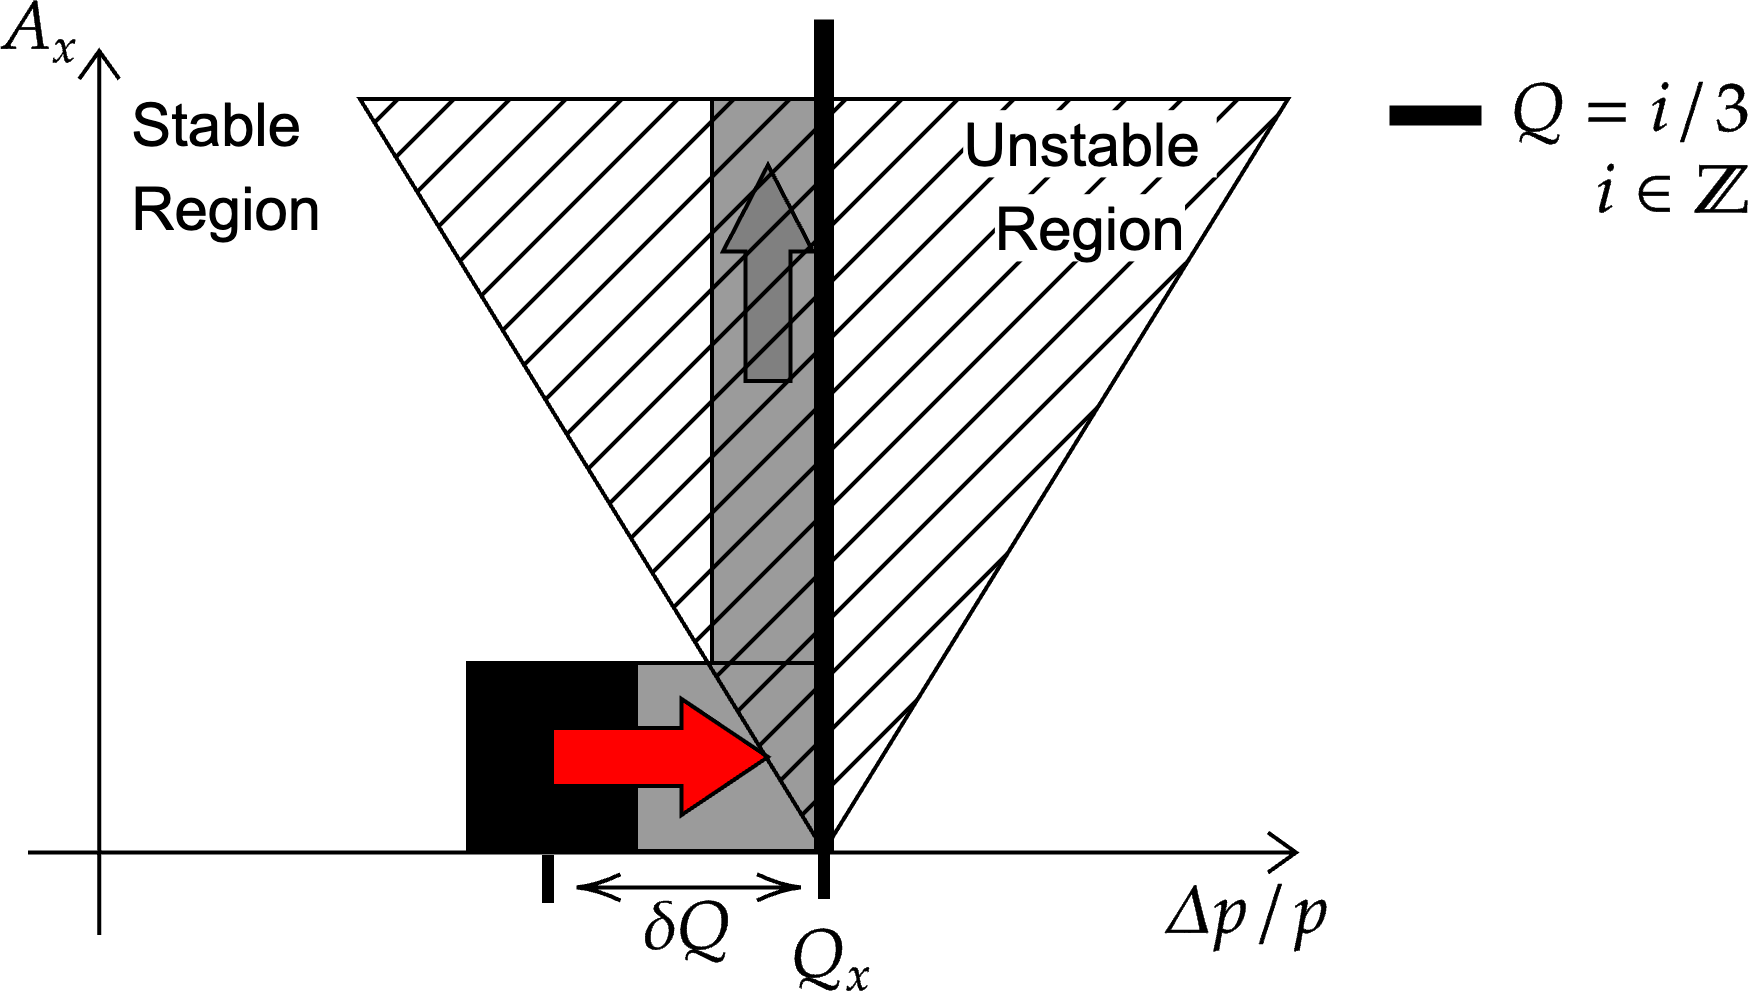
\includegraphics[width=0.6\linewidth]{momentum-driven.png}
  \caption{Steinbach diagram of momentum-driven slow extraction. Waiting beam in black, resonance driving effect in red, unstable beam in grey.}\label{fig:momentum-driven}
\end{figure}

\begin{figure}[ht]
  \centering
  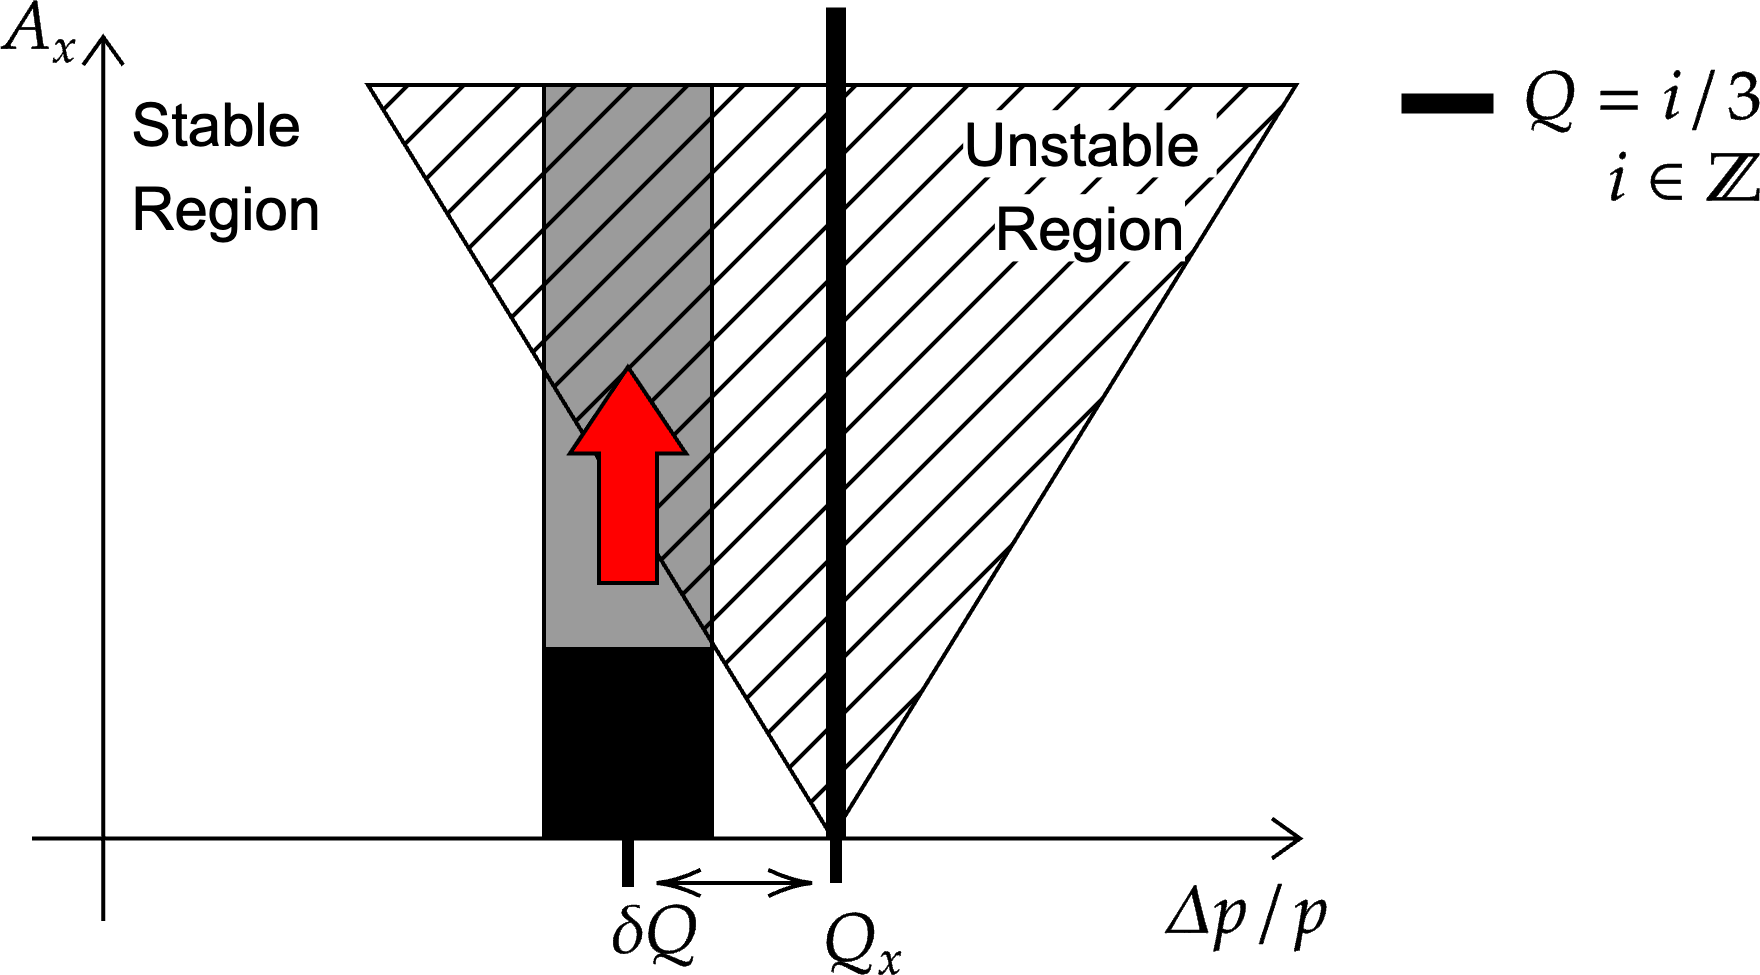
\includegraphics[width=0.6\linewidth]{amplitude-driven.png}
  \caption{Steinbach diagram of amplitude-driven slow extraction. Waiting beam in black, resonance driving effect in red, unstable beam in grey.}\label{fig:amplitude-driven}
\end{figure}

The two beam-moving methods of momentum and amplitude-driven slow extraction can be compared using a Steinbach\footnote{Attributed to C. Steinbach, CERN} diagram. This plots the beam amplitude $A_x$ as a function of momentum $\Delta p/p_0$. The sextupole instability is shown as a triangle, within which is the unstable region beyond the phase-space map separatrices.~\autoref{fig:momentum-driven} and~\autoref{fig:amplitude-driven} illustrate \textit{momentum} and \textit{amplitude} driven slow extraction respectively.
In order for a particle to be considered stable, its single-particle emittance $\epsilon$ must be lower or equal to the area of the separatrix triangle. Using~\autoref{eq:apothem}, this condition is expressed as
\begin{equation}
  A^2\pi\le\frac{48\sqrt 3\pi}{S^2}\delta Q^2\pi
  \label{eq:steinbach}
\end{equation} 
If this condition is plotted on a $(Q, A)$ graph, the stable triangle shown in~\autoref{fig:momentum-driven} and~\autoref{fig:amplitude-driven} is seen. The width of this unstable triangle, known as the \textit{stopband}, is proportional to $S$.

\subsection{Slow Extraction Techniques}\label{sec:rfko}


A variety of slow extraction implementations can be found across particle accelerators. While all will vary to some degree, most can be categorised by which parameter is used to control extraction, and which equipment or magnet is employed. For example:
\begin{itemize}
  \item The \textit{National Center for Oncological Hadrontherapy} (CNAO) uses \textbf{Betatron Core} slow extraction~\cite{Falbo:IPAC2018-TUZGBF3}: a circular magnet produces a longitudinal acceleration, driving particles into 1/3rd-integer resonance.
  \item The \textit{MedAustron} facility has also used \textbf{Constant Optics Slow Extraction} (COSE)~\cite{ArrutiaSota:2845862}, simultaneously scaling the magnetic strength of bending dipoles, and sweeping the betatron tune. This method allows for the alignment of separatrices at different momenta, improving the spill quality.
  \item \textbf{Phase Displacement Extraction} (PDE) allows for resonant extraction without the need for ramping magnetic elements. This avoids pertubations or ramp-rate limits which could arise, and has been tested at both the PS and MedAustron~\cite{ARRUTIASOTA2022167007}.
  \item The \textit{Xi’an Proton Application Facility} (XiPAF) uses \textbf{Radio-Frequency Knock Out} (RFKO) extraction~\cite{Yao:2016cnf}, an amplitude-driven method which transversely ``heats'' (excites) the beam, increasing emittance and amplitude into unstable regions.
\end{itemize}
These accelerators and extraction techniques are mentioned for illustrative purposes: it is not an exhaustive list, and most accelerators can employ multiple methods.
 
The work in this thesis will focus on implementing (and later, simulating) \textit{Radio-Frequency Knock Out} (RFKO) for East Area extraction at CERN. A variety of reasons motivate this: RFKO can be performed with both bunched (particles are longitudinally trapped by RF cavities) and coasting (debunched, particles spread along the entire ring circumference) beams. Performing bunched RFKO allows for the same beam to be re-accelerated and re-extracted multiple times~\cite{russo}. Additionally, this method is typically quicker to respond (i.e. turning on and off extraction) than other methods~\cite{Furukawa2002PROGRESSOR, FURUKAWA200259, NODA2002241}.

RFKO can also be used with an amplitude modulated (AM) excitation, which can be calibrated to provide a constant particle flux over time. However, for the experimental application in this thesis, AM was not used, as the extraction process took place over a long enough time period where flux was not a concern.

The principle of RFKO, as illustrated in~\autoref{fig:rfko_phase_space}, is to excite particles into the resonant instability region by providing transverse ``heating'' of the beam---using a radio-frequency exciter to provide a small transverse kick to the beam, increasing its amplitude. A variety of different signals can be used to drive the excitation: theoretically, white noise (a random signal with equal intensity at all frequencies) would be the ideal signal, providing a purely diffusive effect in phase space. However, pre-existing hardware favours the use of a frequency-modulated ``chirp'' signal, centred at the third-integer fraction of the betatron tune. A range of frequencies around this value is required as there is a range of momenta---and thus a range of tunes---present in the PS East Area beams. 

\begin{figure}
  \centering
  \includegraphics*[width=0.6\linewidth]{rfko-phase-space-schematic.png}
  \caption{A phase-space schematic of RFKO, showing the emittance growth (dashed to solid ellipse) increasing the amplitude of a stable particle (white) into the unstable region (grey), where it moves along the separatrices (arrows) into extraction.}\label{fig:rfko_phase_space}
\end{figure}

\chapter{Implementation and Simulation}

This chapter presents the novel implementation of RFKO slow extraction at the PS, providing a spill to the East Area fixed-target experiments. As motivated in~\autoref{sec:modelling-slow-extraction}, this chapter will also outline the development of simulation models for the RFKO system using existing particle tracking and accelerator optics software. Significant effort was made to streamline the simulation process, leverage the GPU acceleration available in \verb|Xsuite|, and to make full use of the computing platforms available at CERN.

\section{RFKO Slow Extraction at the CERN PS}

For the implementation of RFKO extraction to the East Area, a basic EA-type beam was set up and configured as follows. For preliminary studies, a \qty[per-mode=symbol]{750}{\mega\electronvolt\per~c\per nucleon} Lead (\ch{Pb^{+54}}) ion beam was used, produced by Linac 3 and injected from LEIR. This is the beam configuration used by the CHIMERA experiment, as it provides the correct energy, flux, and beam size for its requirements. After these tests, when an ion beam was no longer available, a proton beam with equivalent magnetic rigidity was used.

This equivalency can be calculated using~\autoref{eq:brho}, \autoref{eq:relativistic_energy}, and \autoref{eq:relativistic_momentum}, producing an equation for the total momentum of an ion beam:
\begin{equation}
  pc=E_0\sqrt{\left( \frac{E_{kin}}{E_0}+1\right)^2-1}
  \label{eq:ion_momentum}
\end{equation} where $E_0$ is the rest mass of the ion, and the relativistic gamma factor $\gamma_c = \frac{E}{E_0}=\frac{E_0+E_{kin}}{E_0}=\frac{E_{kin}}{E_0}+1$.

A (\ch{Pb^{+54}}) ion ($Z=82$ protons, $N=126$ neutrons, $n_e=28$ electrons) at kinetic energy \qty[per-mode=symbol]{750}{\mega\eVperc\per nucleon} will have an atomic mass $A$ of \qty{208}{\atomicmassunit}, and so a kinetic energy of 
\begin{equation}
  E_{kin}=E_{kin/u}*A=\qty{750}{\mega\electronvolt}\cdot 208=\qty{156}{\giga\electronvolt}
\end{equation}
%This ion will have a rest mass of
%\begin{eqnarray}
%  m_{Pb54+}= Z\cdot m_p + N\cdot m_n + n_e\cdot m_e - m_{binding}
%\end{eqnarray} where $m_p, m_n, m_e$ are the masses of a proton, neutron, and electron. The mass defect $m_{binding}$ is found using
%\begin{eqnarray}
%  m_{binding}=Z\cdot m_p + N\cdot m_n + n_e\cdot m_e - A\cdot m_u
%\end{eqnarray} where $m_u$ is the atomic mass unit. 
%These values, when computed, result in a 
and a rest mass of \qty{193.74}{\giga\electronvolt\per\clight\squared}. The equivalent proton momentum, using~\autoref{eq:ion_momentum} and~\autoref{eq:brho}, is then calculated as \qty{5.397}{\giga\electronvolt}. 

Therefore, a single-bunch, low intensity (\qty[per-mode=symbol]{30d10}{particles\per bunch}) \qty{5.397}{\giga\electronvolt} proton beam was chosen, injected to the PS through a single PSB ring (ring 3). The cycle was configured to use two basic beam-cycle periods of \qty{1.2}{\second}, in order to extend the window available for a spill to \qty{500}{\milli\second}.

\begin{figure}
  \centering
  \includegraphics*[width=\linewidth]{ps-sx-system.png}
  \caption{A schematic of the PS Ring and East extraction system, as configured for RFKO slow extraction. All important beamline elements are labelled with their CERN layout code. Also shown is the reference orbit (solid line), the bumped orbit (dashed line) created by the kicker magnets, and the extracted trajectory (double line) created by the magnetic septa.}\label{fig:schematic}
\end{figure}

\subsection{Closed Orbit and Extraction Trajectory}

As shown in~\autoref{fig:schematic}, the closed orbit of the PS at extraction differs to that of the nominal orbit. Four \textit{bump} magnets, (\verb|BSW|) create a large horizontal displacement at the two septa \verb|SMH57| and \verb|SMH61|. This brings the closed orbit within range of the septum blades, where resonant particles can then cross the blade and enter the septum window.

The electrostatic septum, placed before the magnetic septa, is not used in this study, as it is skipped by the beam during ion extraction. It was decided that a proton implementation closer to the ion configuration would be advantageous, so that results can be compared to work carried out by CHIMERA.

\subsection{Cycle Parameters}\label{sec:magcycle}

The dipole magnetic field required for a \qty[per-mode=symbol]{5.392}{\giga\electronvolt\per~c} proton beam is \qty{0.257}{\tesla}, which provides the configuration for the PS Main Unit being magnets. In order to control the third-order resonance, and align the separatrices with the septum blade, the extraction sextupole system was enabled. This consists of a high-level parameter \verb|PR.XSE/K|, which controls the sextupole normalised strength $k_2$ of the two extraction sextupoles, \verb|XSE01| and \verb|XSE07| (\autoref{fig:schematic}). 

A high-level parameter \verb|QSE| is also provided, which controls the normalised strength $k_1$ for a set of extraction quadrupoles (\autoref{fig:schematic}). These serve to aid in betatron tune $Q_x$ control, and to increase the amplitude $\beta_x$ while decreasing the dispersion $D_x$ at the septa locations. This large $\beta_x$ allows the septum to be placed further from the circulating beam, and the small dispersion $D_x$ aligns the separatrices at different momenta along the septum blade. These two parameters \verb|QSE| and \verb|XSE|, have been pre-configured for nominal East Area slow extraction.

The high-level tune control knobs were also configured for RFKO. These use the Pole Face Winding (PFW) magnets present in every PS Main Unit dipole to control the horizontal and vertical betatron tunes $Q_{x, y}$ and chromaticities $Q'_{x, y}$. Tune control was very important to the set-up of this implementation---the horizontal tune was positioned close to the third-order resonance, at 0.32. The chromaticity was minimised to avoid part of the circulating beam being brought into resonance before the RFKO system was activated, which would cause a low-level initial uncontrolled spill. This tune control is shown in~\autoref{fig:tunemap}, which plots vertical tune against horizontal tune. This provides a convenient visualisation of first, second, and third order resonances. These resonances are defined by
\begin{equation}
  m\cdot Q_x+n\cdot Q_y=p
\end{equation} where $m$, $n$, and $p$ are arbitrary integers, where $|m|+|n|$ defines the resonance order. Also used is the fractional tune split, $\Delta$, defined as
\begin{equation}
  \Delta = Q_x-Q_y-p
\end{equation}
From~\autoref{fig:cycle}, we find the tune split at injection $\Delta=-0.1$, and at extraction $\Delta=0.07$, both of which avoid coupling resonances.

\begin{figure}
  \centering
  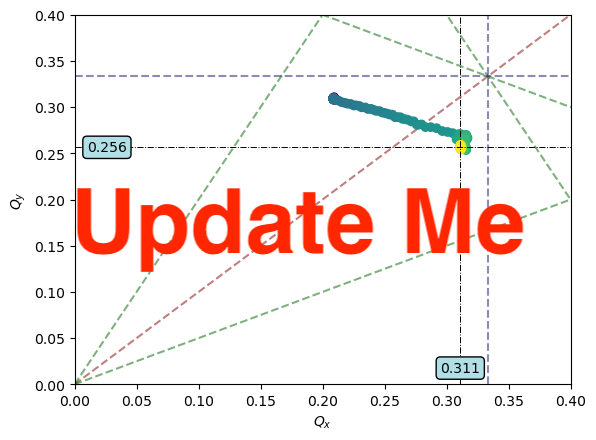
\includegraphics[width=0.6\linewidth]{tunemap.png}
  \caption{A fractional tune map, plotting the evolution of horizontal fractional tune $Q_x$ against vertical fractional tune $Q_y$. Color scale indicates time. Dashed lines indicate some of the first order (red), second order (green) and third order (blue) resonances. Black lines at $Q_x=0.319, Q_y=0.249$ are the final tunes reached at the extraction period. Integer part for all tunes is 6.}\label{fig:tunemap}
\end{figure}

\begin{figure}[h]
  \centering
  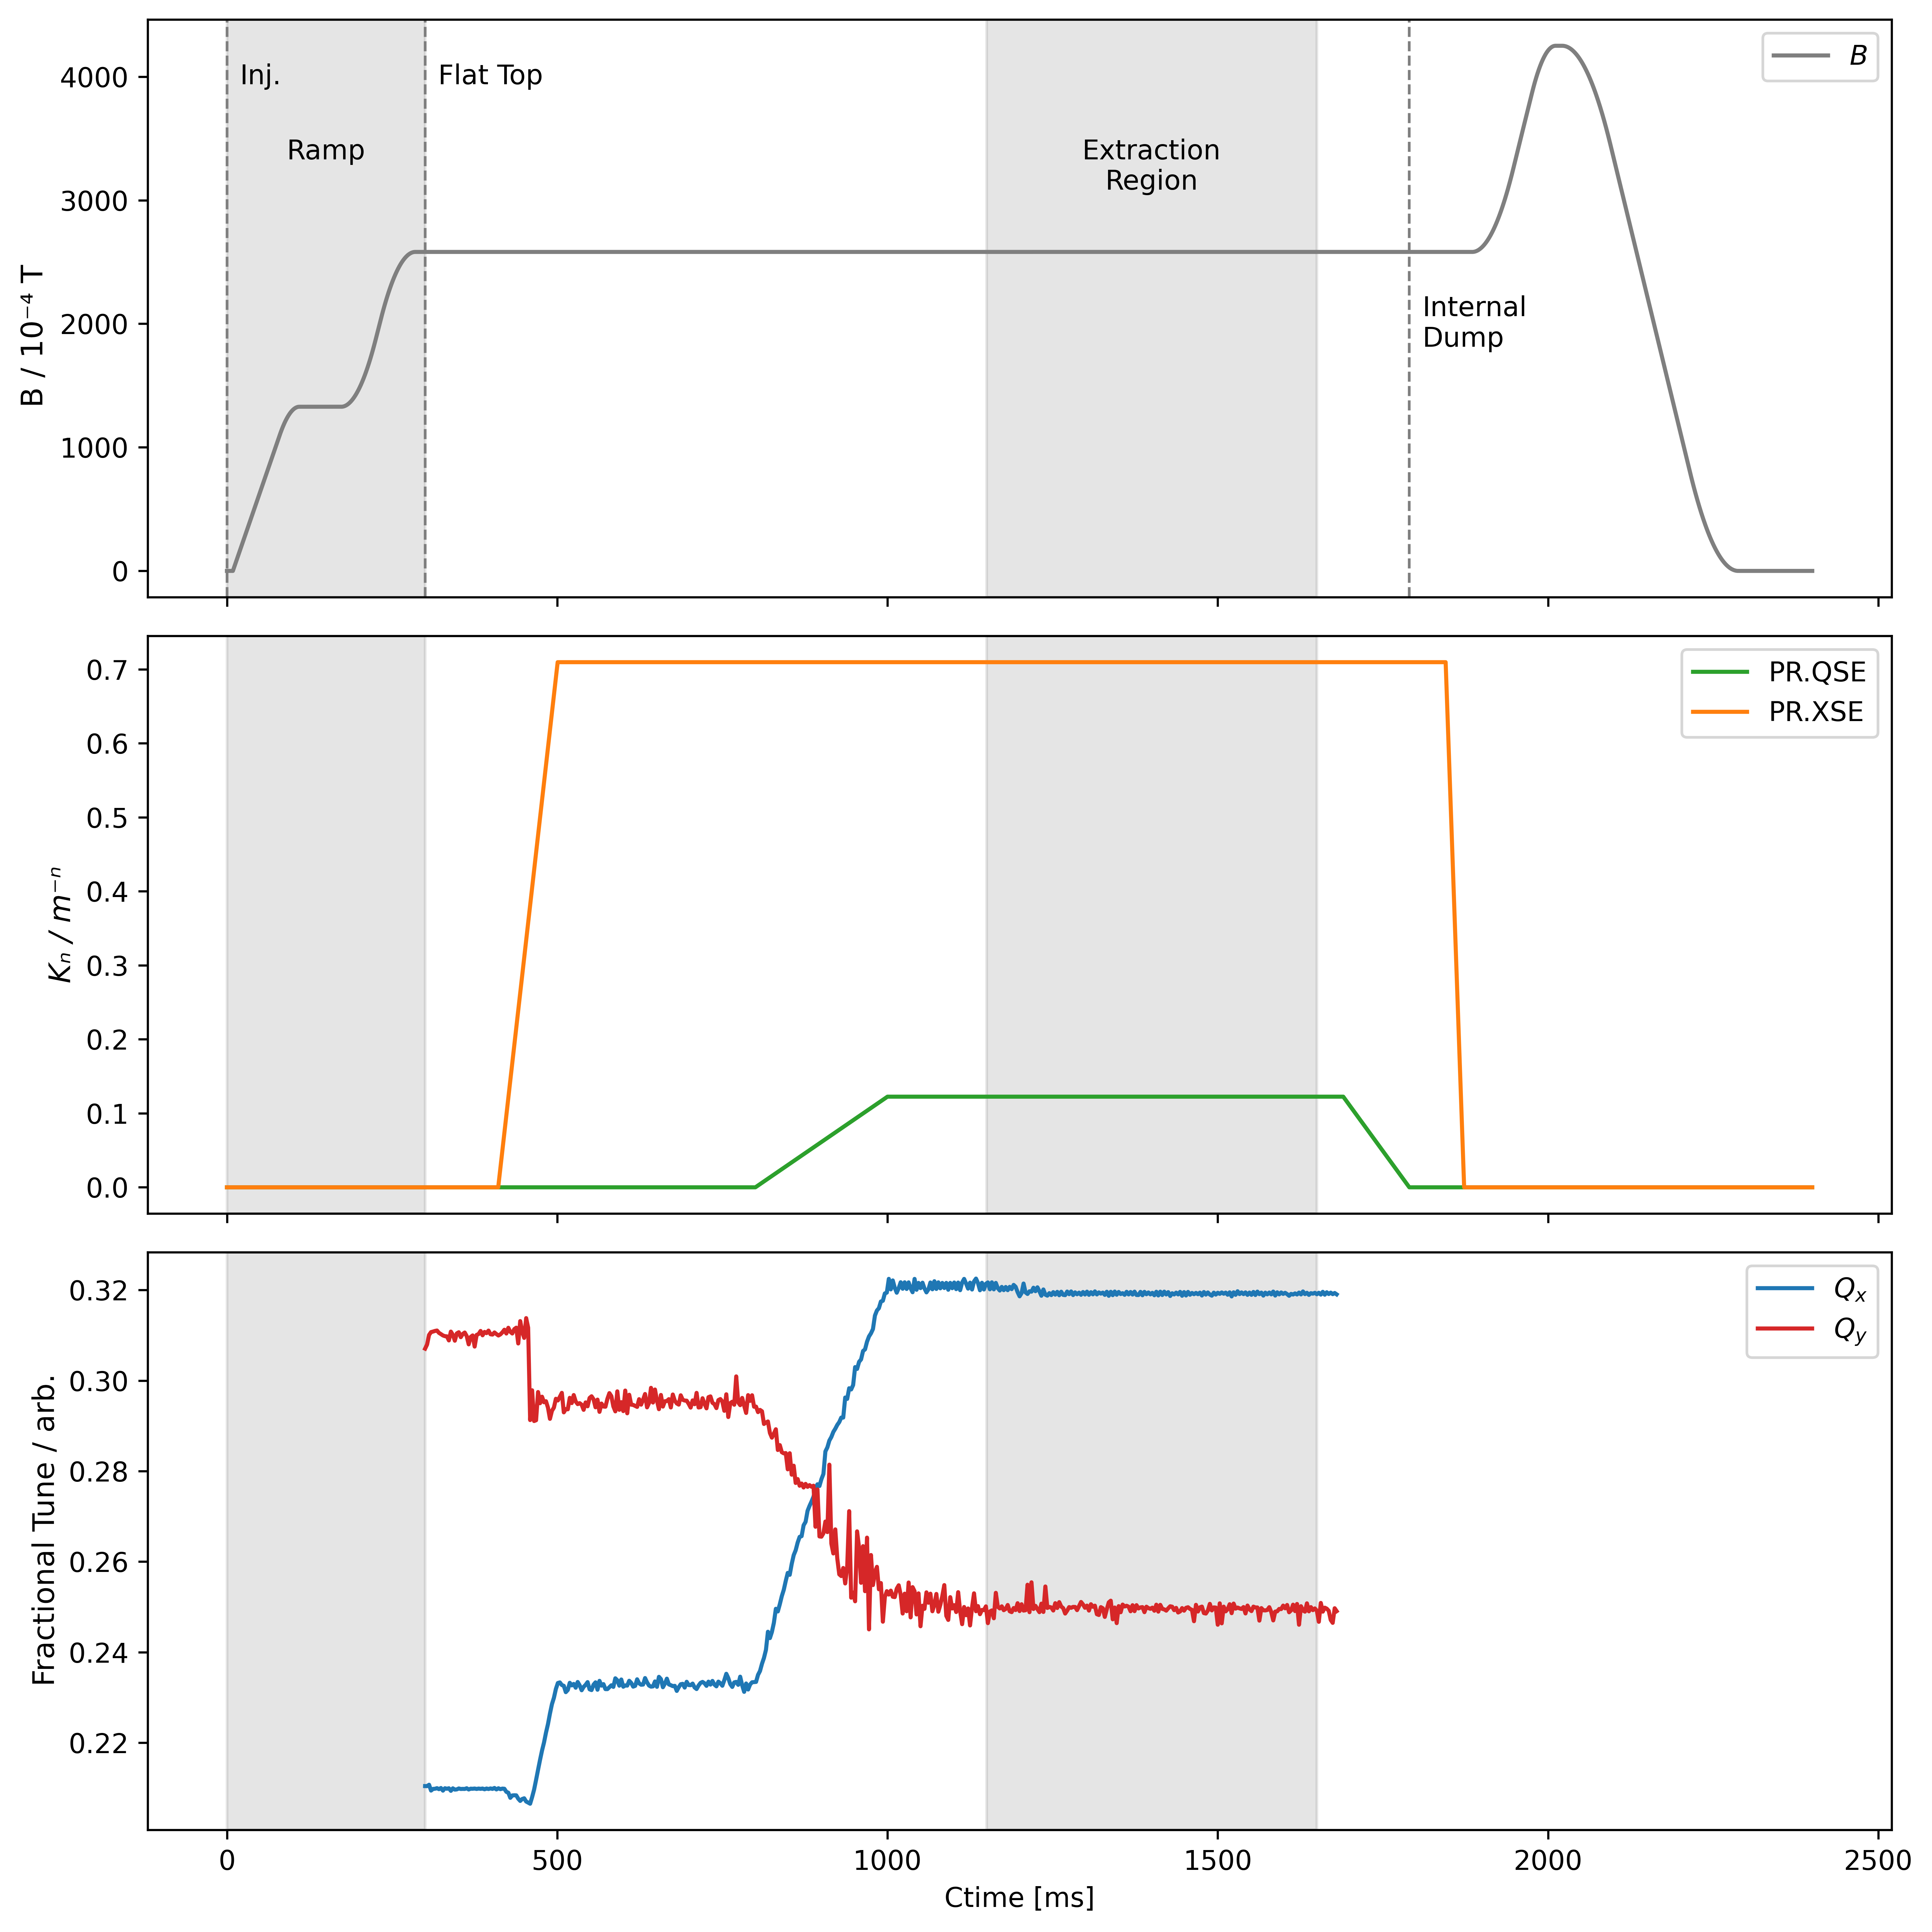
\includegraphics[width=0.9\linewidth]{cyclegraphs.png}
  \caption{The high-level parameter configuration for the implementation of East Area RFKO slow extraction. Top graph shows the bending dipole $B$ field, points of injection (from PSB) and dumping (internal absorption of remaining beam), and regions of acceleration (ramp) and stable period for extraction. Second graph shows multipole components $k_n$ for extraction quadrupole ($k=1$) and sextupole ($k=2$). Final graph shows fractional betatron tune measurements for horizontal and vertical plane.}\label{fig:cycle}
\end{figure}

The RF system in the PS (\autoref{sec:long}) is used to accelerate the beam up to \qty{5.392}{\giga\electronvolt} during the \textit{ramp} period, and to maintain bunching during \textit{flat-top}. An East-type beam in the PS is bunched at the \nth{8} harmonic, or can be disabled to \textit{debunch} the beam (known as a coasting beam). RFKO can be performed with both a bunched and coasting beam, and both scenarios will be examined.

\subsection{Transverse Excitation}\label{sec:trans_exc}
Once a basic, stable cycle is configured in the PS, the transverse excitation is implemented. This uses a transverse kicker located at section 97 of the PS, \verb|KFB97|, a $\sim$\qty{1}{\meter} long strip-line kicker, with both horizontal and vertical planes~\cite{Sterbini:2158994}. With a peak RF power of \qty{5000}{\watt} across the two electrodes, and an impedance of \qty{100}{\ohm}, the transverse feedback (TFB) kicker can provide a peak voltage at \qty{1000}{\volt} and current of \qty{10}{\ampere}. The electric and magnetic fields are then defined as:
\begin{equation}
  E=\frac Vr
\end{equation}
\begin{equation}
  B=\frac {2I}{2\pi r}\cdot \mu_0
\end{equation}
where $r$ is the electrode aperture \qty{70}{\milli\meter}. The electric and magnetic deflection angles are then~\cite[3.1-3.2]{bouvet}
\begin{equation}
  \theta_E = \frac{E \cdot L}{p\cdot\beta}
  \label{eq:kick-electric}
\end{equation}
\begin{equation}
  \theta_B = \frac{B\cdot L}{p}
  \label{eq:kick-magnetic}
\end{equation} where $L$ is the electrode length \qty{935}{\milli\meter}. The stripline components $B$ and $E$ both contribute to the kick, and so the summation of these two angles provides a maximum deflection of \qty{10.814605}{\micro\radian}.

To drive this transverse kicker, two systems were used. Initially, the \verb|Qmeter| control program~\cite{Gasior:895142} provided an interface to this kicker. While the program was designed---and used extensively in this study---for tune measurements, it can be exploited to provide a frequency-modulated \textit{chirp} signal crossing the \nth{3}-order resonance to the TFB plates. The program was used to configure the \textit{start} and \textit{stop} frequencies for the frequency-modulated chirp (as unit interval multiples of the revolution frequency $f_{rev}$), chirp length (in $2^n$ revolutions), and the time after which the chirp would repeat (in milliseconds). This produced the effect of a repeated frequency-modulated chirp windowed by a square signal (\autoref{fig:qmeter-signal}). Previous studies~\cite{ipac} found suitable parameters to produce a baseline RFKO extraction implementation, tabulated in~\autoref{tab:qmeter-params}, and found a significant dependency of spill quality on the chirp repetition rate.

\begin{table}[]
  \centering
  \begin{tabular}{ll}
    \centering
  Parameter                 & Value                  \\ \hline \hline
  Chirp Start $[Hz]$        & $0.3\cdot f_{rev}$     \\
  Chirp Stop $[Hz]$         & $0.35\cdot f_{rev}$    \\
  Chirp Repetition $[ms]$   & 1                      \\
  Chirp Turns               & 256                   
  \end{tabular}
  \caption{Initial parameters for RFKO extraction using the \textit{Qmeter} control program.}\label{tab:qmeter-params}
\end{table}

\begin{figure}
  \centering
  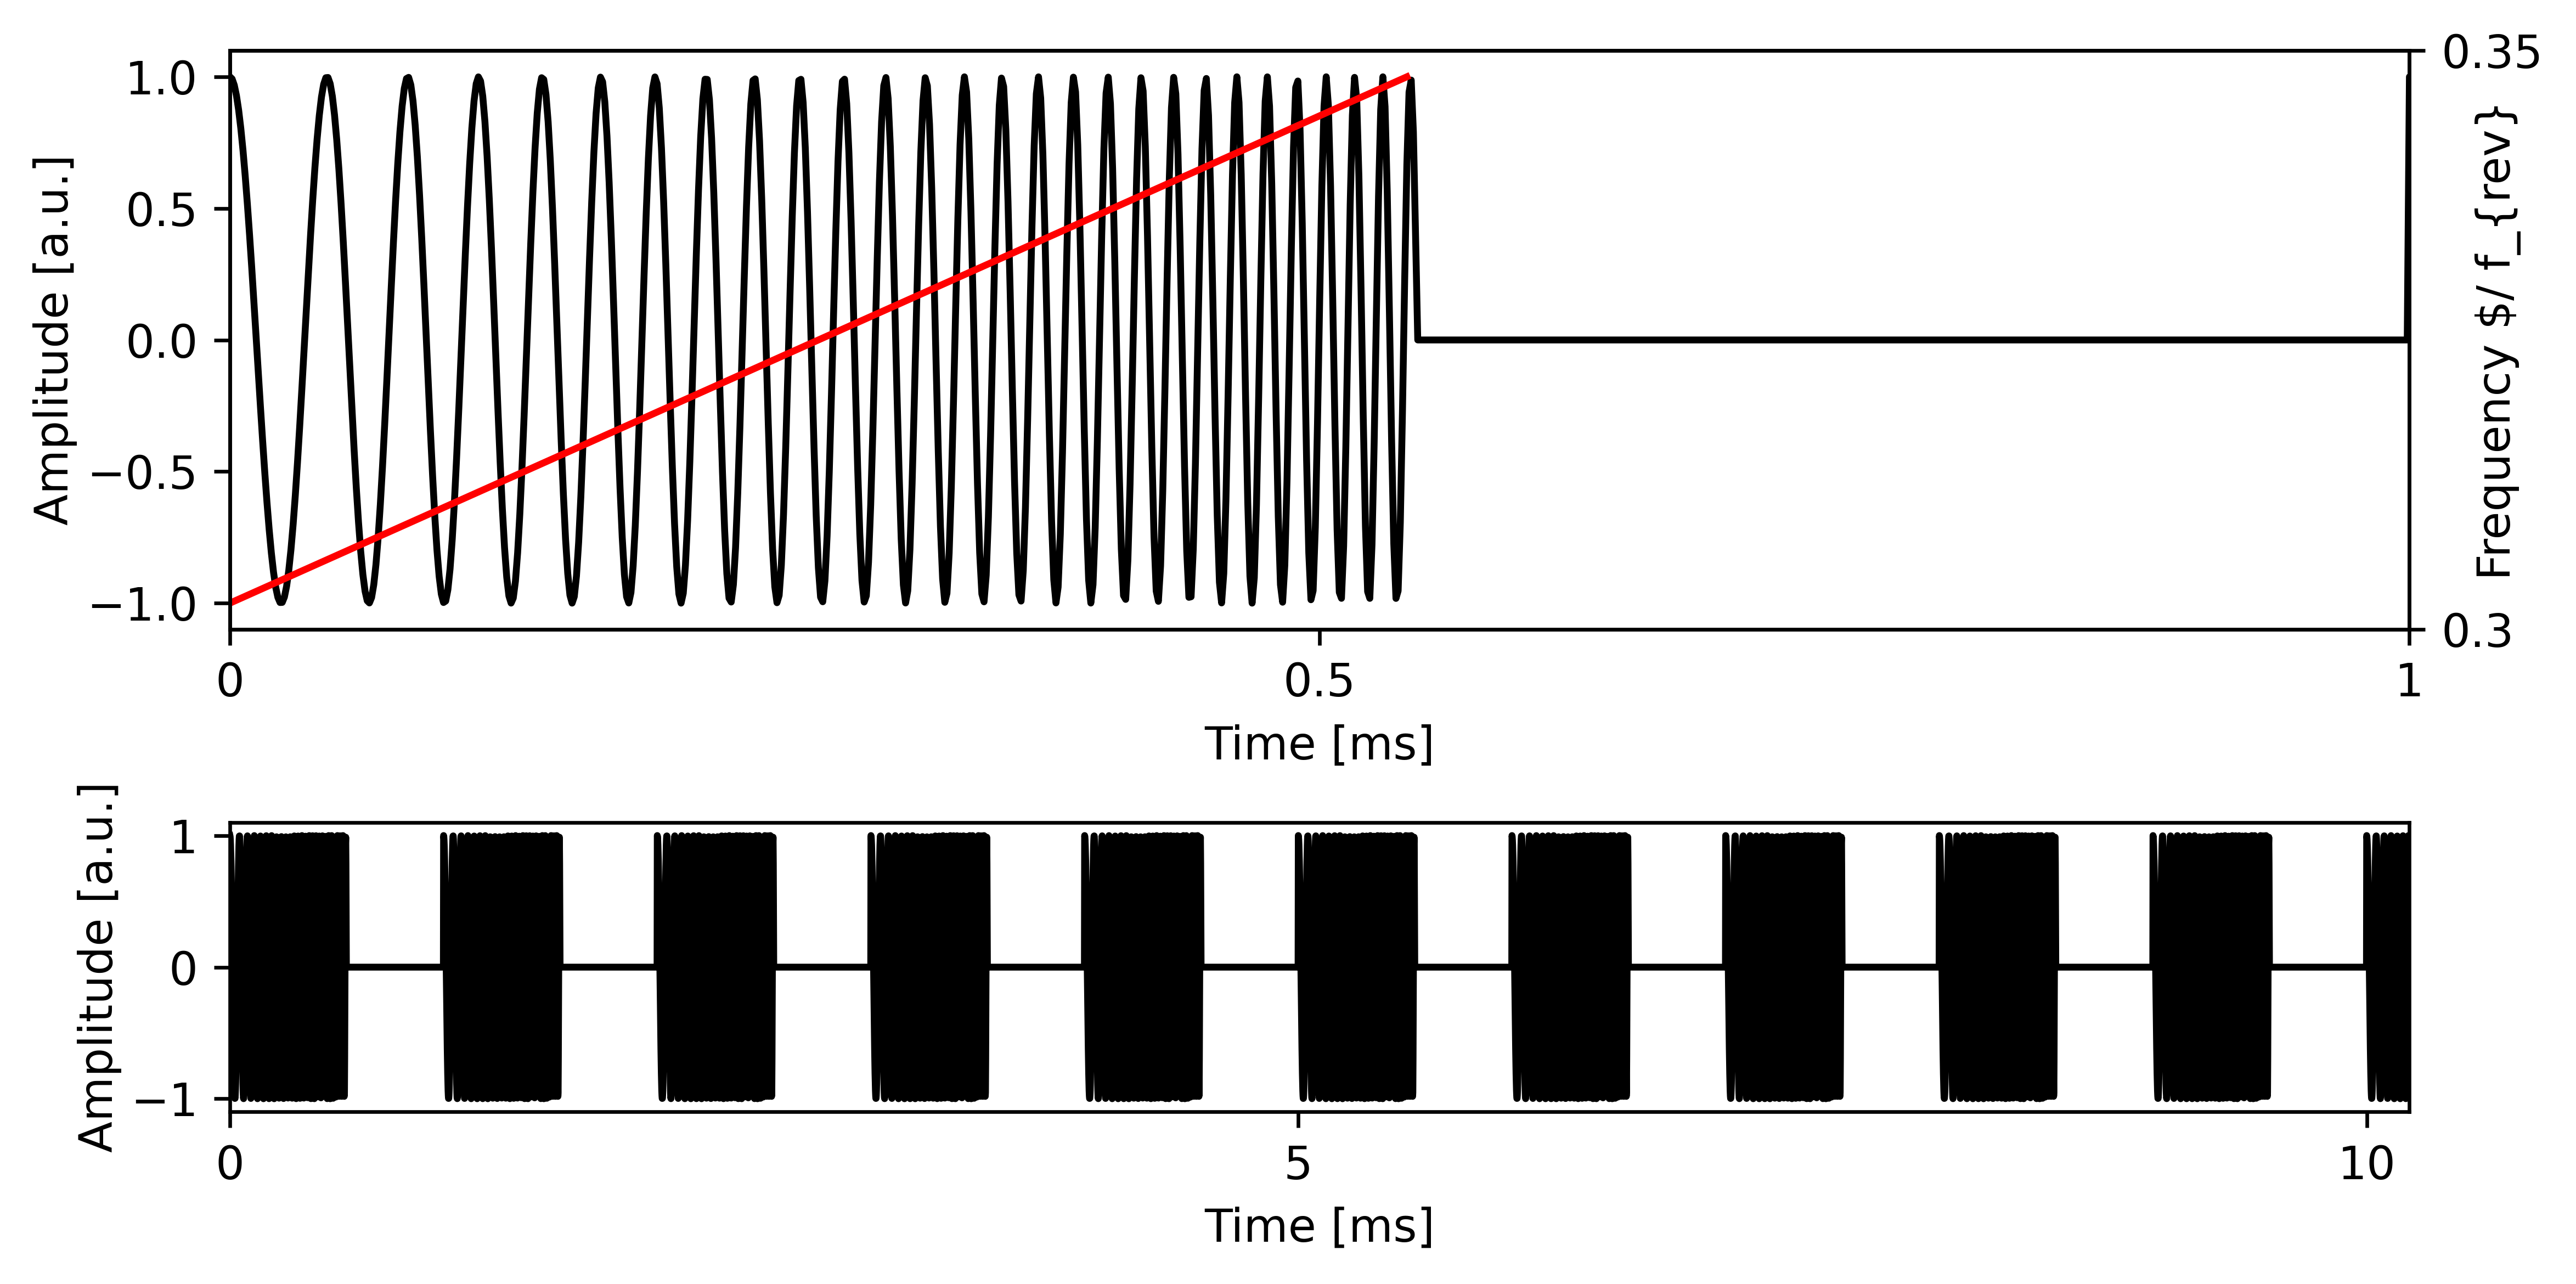
\includegraphics[width=0.6\linewidth]{fake-signal.png}
  \caption{An example of the chirp signal generated by the \textit{Qmeter} application; a frequency-modulated chirp windowed by a square signal. Top plot shows the signal (amplitude, black) and frequency modulation (red) in the time-frame of one repetition. Bottom plot shows multiple repetitions over the span of 10 ms.}\label{fig:qmeter-signal}
\end{figure}

To explore chirp repetition rates above the \qty{1}{\kilo\hertz} (below \qty{1}{\milli\second}) limit of \verb|Qmeter|, a new signal generator was configured to control the TFB kicker plates. This function generator was configured as a two-channel source, channel 1 being a sine wave with a frequency modulated by channel 2, a ramp/sawtooth wave. By choosing a central frequency and frequency deviation corresponding to the chirp generated by \verb|Qmeter|, the function generator was able to produce a similar signal to that of the \verb|Qmeter| system, but not windowed by a square function (\autoref{eq:both-chirps}). This allowed for chirp repetition rates of \qty{1}{\kilo\hertz} and above, and was used to explore the effect of chirp repetition rate on spill quality.

\begin{figure}
  \centering
  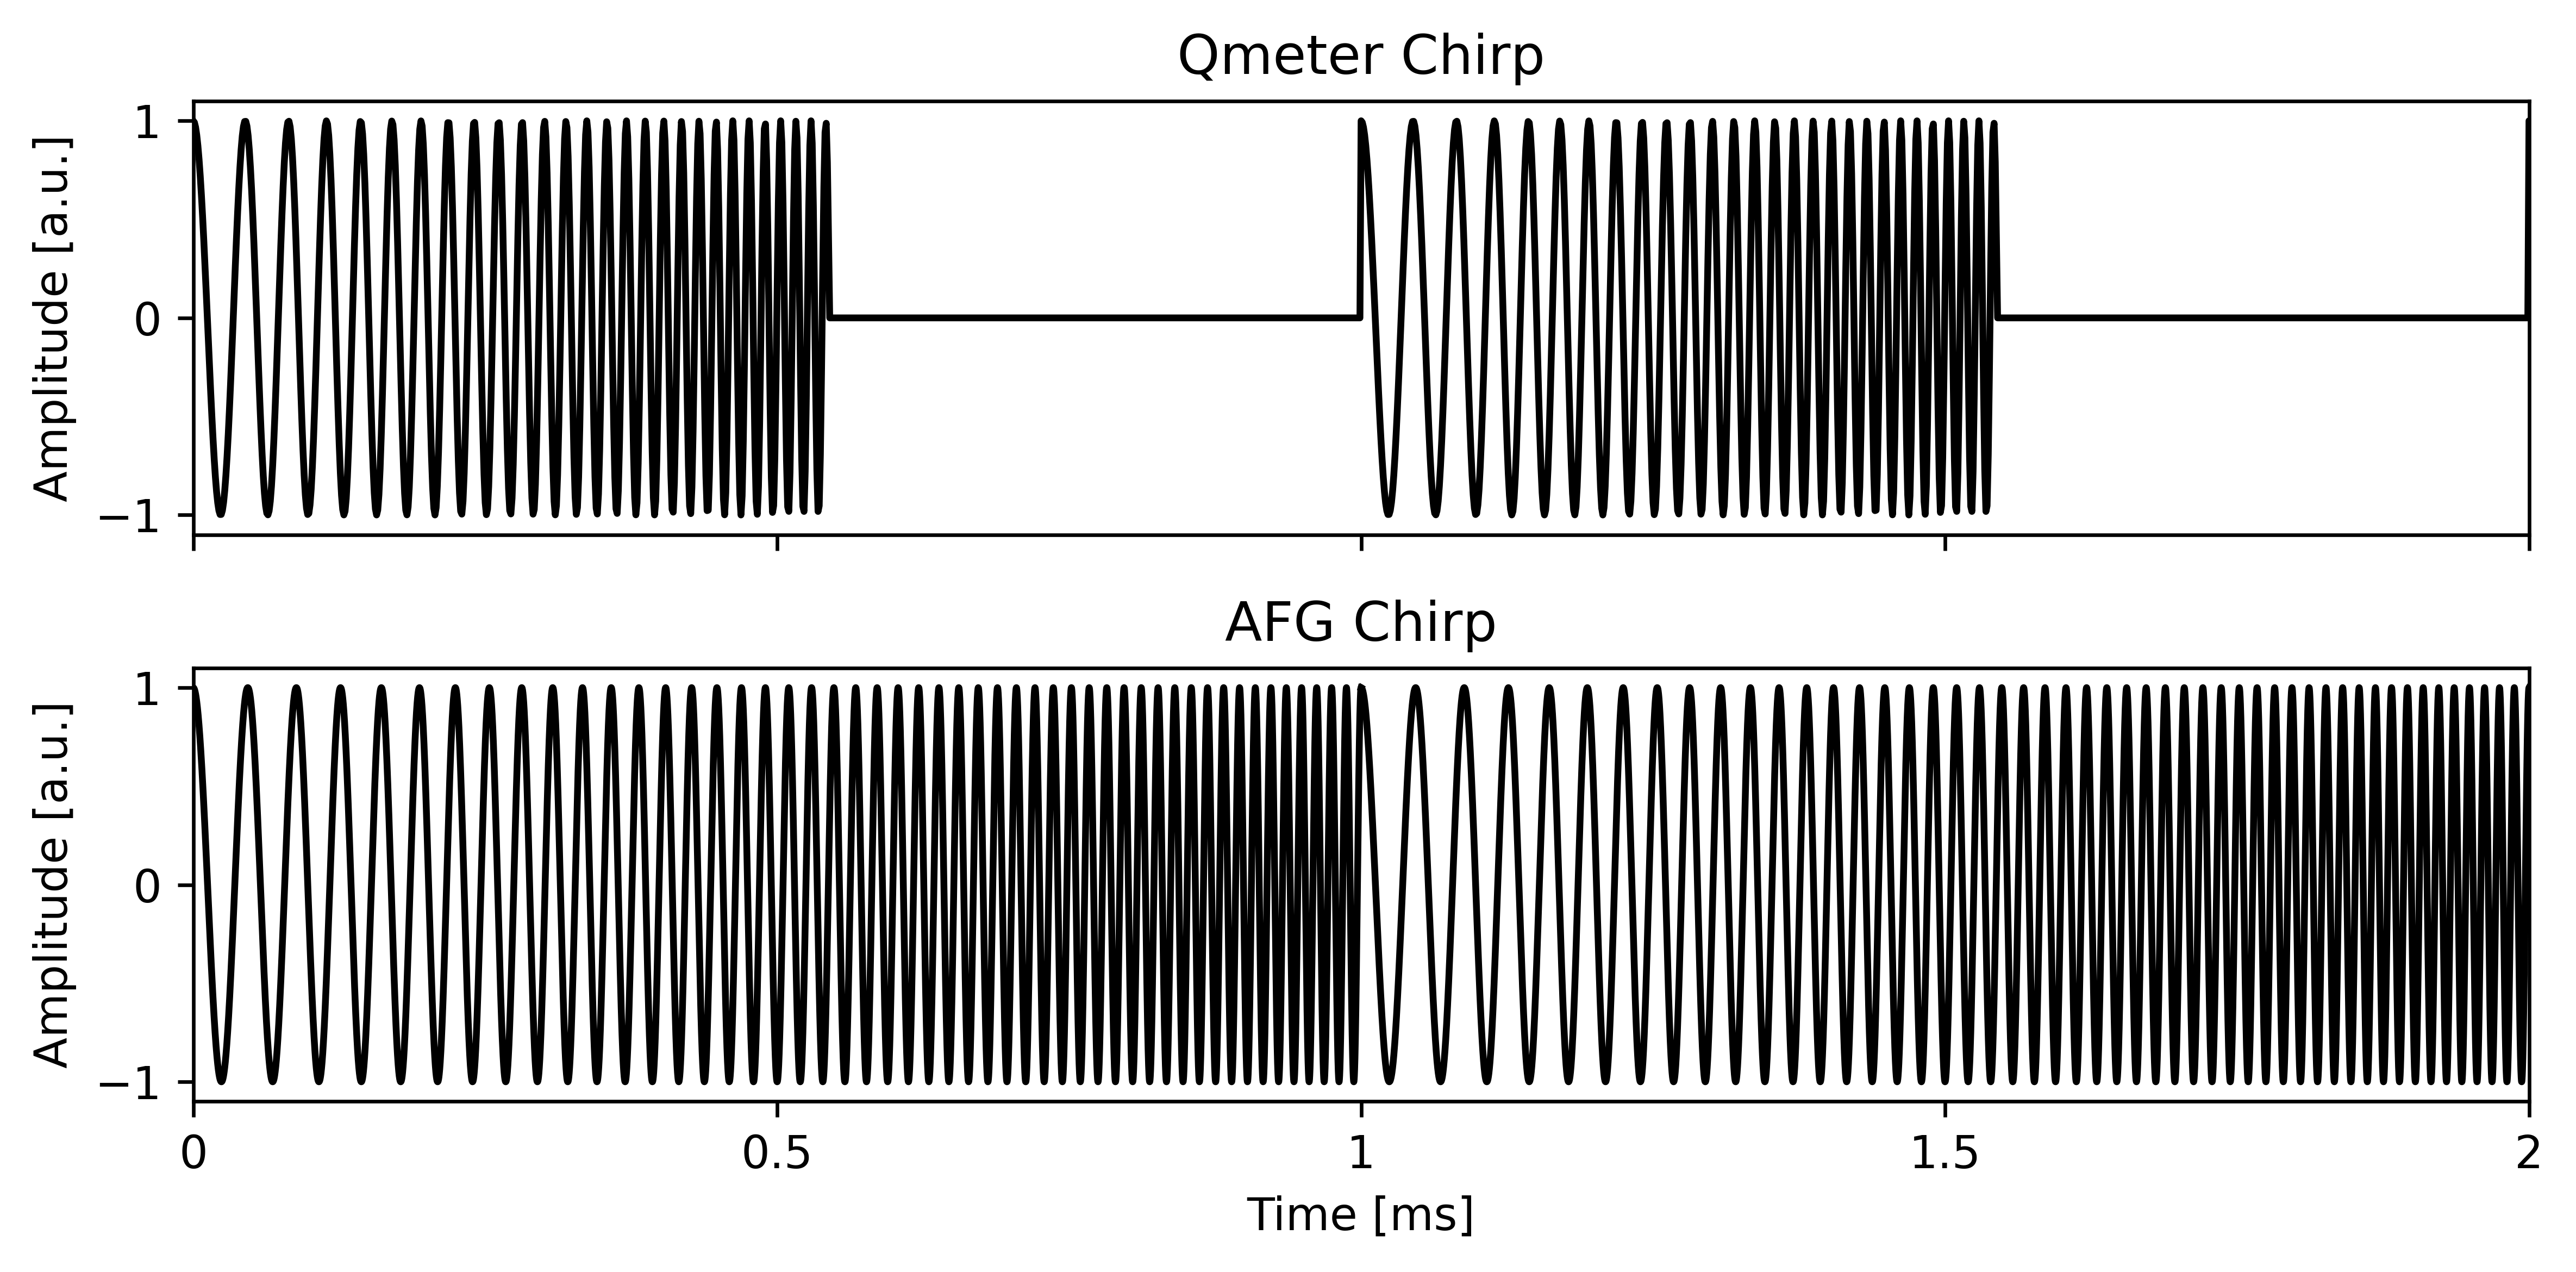
\includegraphics[width=0.6\linewidth]{both-chirps.png}
  \caption{An example of the chirp signal generated by \textit{Qmeter} (top) and by the arbitrary function generator (AFG) (bottom).}\label{eq:both-chirps}
\end{figure}

To aid in the research in this paper, and future use-cases of RFKO at the PS, a package was written to simplify the interface with the AFG via the \textit{Standard Commands for Programmable Instruments} (SCPI) protocol. This interface---available as part of the \textit{CERN General Devices} package~\cite{cgd}---configures the AFG for RFKO extraction, and provides a Python class for modifying the chirp-generation parameters in terms of the revolution frequency $f_{rev}$, and the chirp length in milliseconds. This package was used to control the AFG for the results presented in this paper.


\section{Modelling RFKO Slow Extraction}\label{sec:rfko_sim}

As motivated in~\autoref{sec:motivation}, the majority of work surrounding the results presented in this thesis was towards developing a simulation framework to accurately model the spill structure of RFKO at the PS. This section will detail the simulation tools used, the implementation of the RFKO extraction simulation, and the methods used to compare the simulation results to machine data.

\subsection{Simulation Tools}

A variety of simulation software packages for accelerator physics are available, each having their own optimisations, and application areas amongst the accelerator physics community. For this study, the \verb|MAD-X|~\cite{Iselin:MAD} and \verb|Xsuite|~\cite{xsuite} packages were used.~\verb|MAD-X| is a common tool in the area of optics and beam transfer, and CERN provides a common optics repository---\verb|acc-models|~\cite{optics_repo}---containing \verb|MAD-X| \textit{sequence} files which describe the optics lattices for the CERN accelerator complex. For the PS, many \textit{scenarios} are provided alongside the operational models, one of which is a pre-configured for East Area slow extraction.

\verb|Xsuite|---a relatively recent simulation tool, first made available in 2021---is a Python package which shares many similarities with \verb|MAD-X|, and can import \verb|MAD-X| sequences into its own lattice definitions. However, \verb|Xsuite| has additional capabilities, such as \textit{context} management, which provides the ability to run simulations on different hardware---namely GPUs. This is achieved by using the \verb|cupy|~\cite{CuPy} package, which provides a drop-in replacement for \verb|numpy|, but with optimisations for accelerating workloads on GPUs. Additionally, \verb|Xsuite| has an existing \verb|Exciter| beam element, which can model the time-dependent transverse kicker used in RFKO. There has been a rapid increase in the use of \verb|Xsuite| within the accelerator physics community at CERN, which---combined with the additional capabilities beyond \verb|MAD-X|---motivated its use in this study.

\subsection{Lattice Configuration} % needs a better title

The \textit{East Area Extraction} scenario provided by \verb|acc-models| was used as the basis for all simulation models, and was modified to include the parameters outlined in~\autoref{sec:magcycle}. This generated lattice file---defining the strengths and location for all 1326 beam elements---was used to produce the optics plots shown in~\autoref{fig:acc-models-optics}, which displays how the kicker magnets create large displacements at the extraction septa, and how dispersion is controlled by the extraction quadrupoles.

\begin{figure}[h]
  \centering
  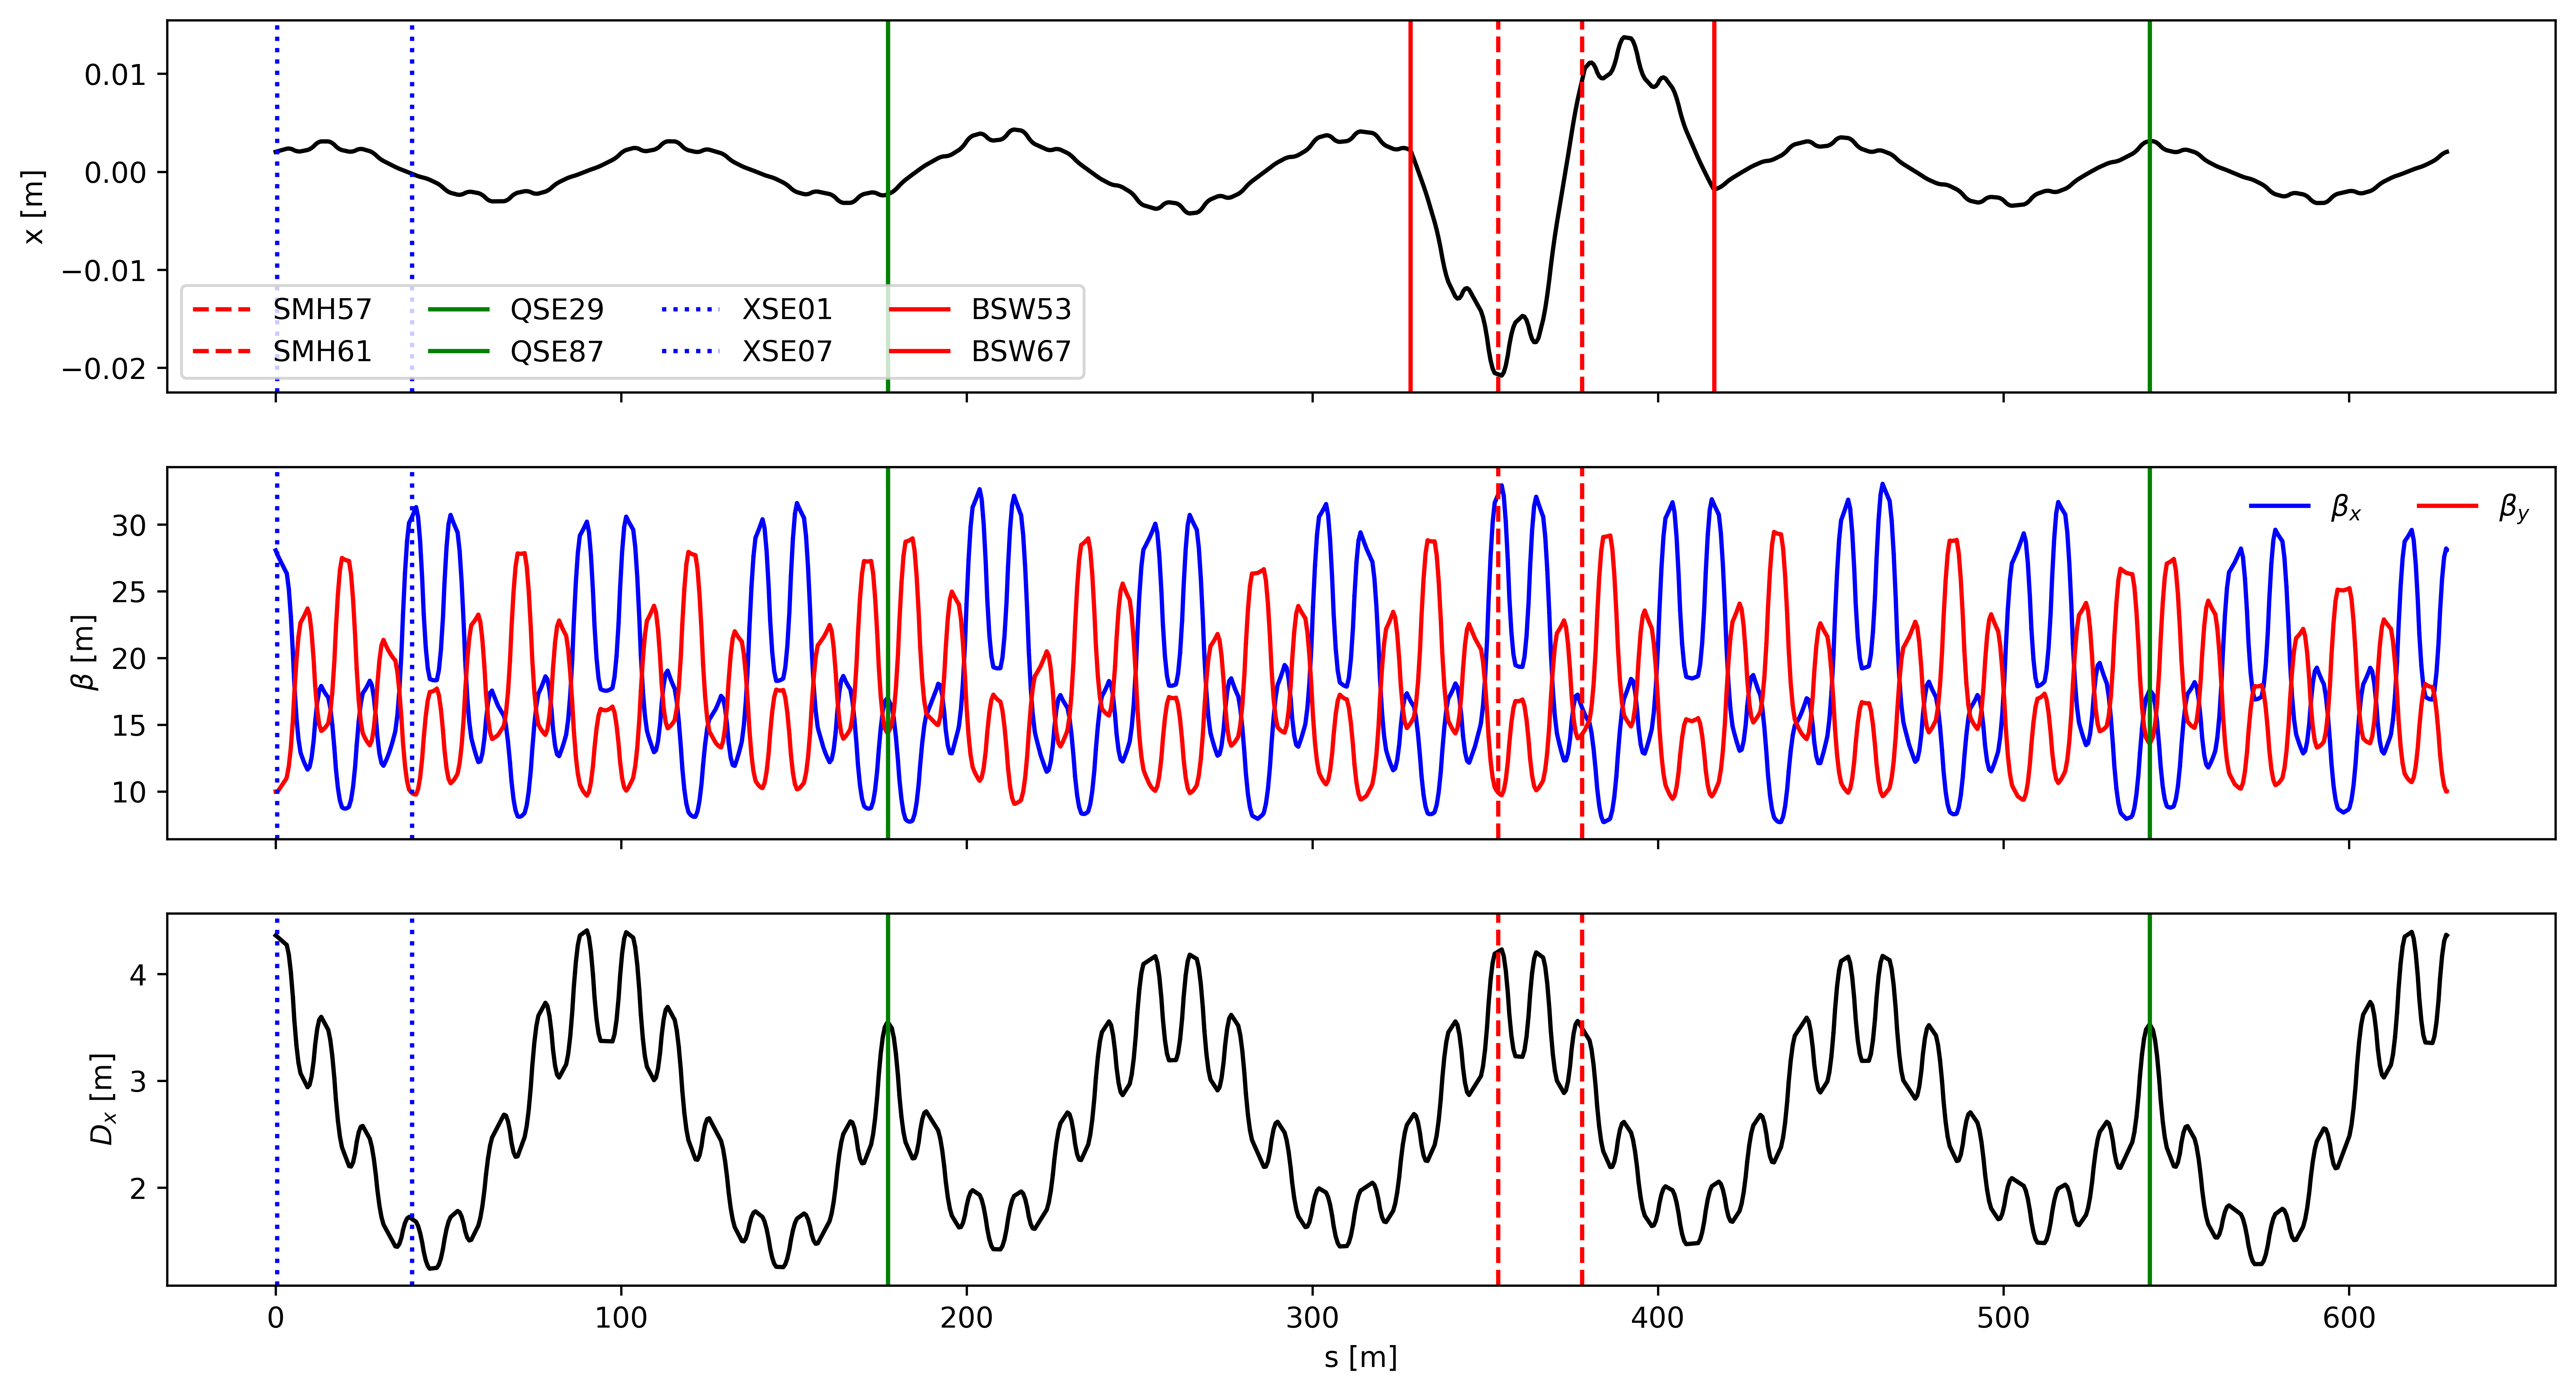
\includegraphics[width=0.9\linewidth]{optics.png}
  \cprotect\caption{Optics plots of the closed orbit for the \verb|acc-models| PS East Area extraction scenario. Top figure shows horizontal closed orbit $x$, middle figure shows Twiss beta function $\beta$, and bottom figure shows transverse dispersion $D_x$. Also labelled are key extraction elements: the magnetic septa (\verb|SMH|), the extraction quadrupoles (\verb|QSE|), extraction sextupoles (\verb|XSE|), and kickers (\verb|BSW|)}\label{fig:acc-models-optics}
\end{figure}

This lattice was then imported to \verb|Xsuite|, where the custom RFKO beam elements could be included. These elements were:
\begin{itemize}
  \item An \verb|Exciter|, modelling the TFB kicker \verb|KFB97|.
  \item A \verb|LimitRect|, modelling the magnetic septum \verb|SMH57|.
  \item A \verb|Cavity|, modelling the RF cavities providing acceleration and longitudinal focusing, operating at the \nth{8} harmonic.
\end{itemize}

\subsubsection{Exciter}
Using~\autoref{eq:kick-electric} and~\autoref{eq:kick-magnetic}, a function (\autoref{lst:kick_angle}) was written to convert the voltage applied across the TFB kicker to the angle of deflection generated by the electric and magnetic fields. This value was then used to define the strength of the \verb|Exciter| element, which was placed at the location of the TFB kicker in the lattice. Another function (\autoref{lst:generate_chirp}) was written to generate the chirp signal as generated by \textit{Qmeter} and the AFG. This function was then used to define the \verb|Exciter| element's \verb|samples| parameter, which is used to define the time-dependent kick. 

\subsubsection{Septum}\label{sec:septum}
The first magnetic septum, \verb|SMH57|, was modelled as a simple rectangular aperture \verb|LimitRect|. By setting this aperture to coordinates corresponding to the window of the septum, particles which are lost to the aperture can be considered as extracted. In the real machine, particles recieve two magnetic septum kicks, from \verb|SMH57| and \verb|SMH61|, but this study only considered the first septum to simplify the model and avoid simulating lost particles for longer than necessary. As only one aperture is modelled, it can be assumed that particles lost to an aperture limit---with \verb|Xsuite| particle state \verb|0| (flag \verb|XT_LOST_ON_APERTURE|)---entered the window of the septum and were extracted. 

\subsubsection{RF Cavity}

A single RF cavity was added to the model, corresponding to the RF system of the PS. While the real system comprises of many such cavities, modelling a single cavity with the total RF voltage applied provides an accurate representation of the longitudinal dynamics of the beam, given that there are no other longitudinal elements present in the model.

\subsection{Distribution Generation}

To accurately simulate the conditions used in the RFKO studies, the initial particle distribution must be generated using machine measurements. The parameters used included:
\begin{itemize}
  \item Beam momentum $p$ [\si{\giga\eVperc}]
  \item Intensity $I$ [\si{proton \per bunch}]
  \item Horizontal RMS emittance $\varepsilon_x$ [\si{\milli\meter\milli\radian}]
  \item Longitudinal RMS emittance $\varepsilon_s$ [\si{\electronvolt\second}]
\end{itemize}  

These values were obtained during machine studies. The beam momentum and intensity were fixed values, configured by high-level machine parameters. The horizontal emittance $\varepsilon_x$ was measured using Secondary Emission Monitor (SEM) grids~\cite{Martini:324553}, and the longitudinal emittance $\varepsilon_z$ using tomography of the beam current profile~\cite{Hancock:960231}. The measured values are shown in~\autoref{tab:initial-conditions}. The beam distribution was then generated according to these parameters, and ``matched'' to the model longitudinal dynamics of the model by \verb|Xsuite|. An example of the generated distribution is shown in~\autoref{fig:initial-dist}.

It was decided that the simulation code will generate a new distribution each time it was initiated, rather than loading a pre-generated distribution from a file. This was done to allow for the random distributions to be generated with a different random seed each time, avoiding the same distribution being used for each simulation which could introduce bias in the results. This also allowed for the particle generation parameters to be dynamically adjusted on a per-simulation basis, enabling the testing and optimisation of these parameters. This design choice ensured the simulation code was flexible and could be used for a wide range of studies at different beam energies and intensities.

With a sufficiently large number of particles, these random distributions will be statistically similar. This obviated the need to transfer a large, persistent file to each simulation job; this transfer time was, qualitatively, found to be longer than the time taken to generate a new distribution file of the same size.

\begin{table}[]
  \centering
  \begin{tabular}{ll}
    \centering
  Parameter                                       & Value \\ \hline \hline
  Beam Momentum $p$ [GeV/c]                       & $5.392$ \\
  Intensity $N$ [proton/bunch]                    & $3\times10^{11}$ \\
  Transverse Emittance $\varepsilon_{x,y}$ [mm mrad]  & $2.38$ \\
  RMS Longitudinal Emittance [eVs]                & $0.276$
  \end{tabular}
  \caption{Initial parameters particle generation, corresponding to measurements made during machine studies.}\label{tab:initial-conditions}
\end{table}

\begin{figure}
  \centering
  \includegraphics*[width=\linewidth]{initial-dist.png}
  \cprotect\caption{Examples of initial distributions generated by \verb|Xsuite|, for number of particles $N_p=3000$, with parameters as shown in~\autoref{tab:initial-conditions}. Also plotted on each are the $1\sigma, 2\sigma, 3\sigma$ emittance ellipses, and the closed orbit particle (red). Top plots show transverse phase space distribution for all simulation types. Bottom plots show longitudinal phase space distribution for a \textit{bunched} (RF system active) beam (left) and \textit{debunched} (RF inactive) beam (right).}\label{fig:initial-dist}
\end{figure}

\subsection{Simulation Process}\label{sec:sim_process}

Once an initial simulation process was built, one issue became immediately apparent: to simulate the full \qty{0.5}{\second} extraction region (\autoref{fig:cycle}), the simulation needed to process approximately 235,000 turns. To produce a statistically significant extraction rate, a sufficient number of particles---roughly 500,000---needed to be generated and simulated. A typical desktop computer, for instance, would require over 600 hours to complete such a simulation, at a rate of roughly \qty{13}{\second\per iteration}.

To accelerate the simulation speed to a more reasonable rate, two tools were employed. While not unique to Xsuite, they are both simplified by the package. The first method was the simplest: as mentioned previously, \verb|Xsuite| provides ready-to-go compatibility with \verb|CuPy| and CUDA GPU acceleration. The second method relies on CERN's Batch Service, a high-throughput computing service which allows users to submit jobs via the \textit{HTCondor} framework. 

To submit the simulation jobs to the batch processing service, the simulation software was \textit{containerised} using a Docker~\cite{merkel2014docker} image. This image provides a complete environment for the simulation, including a distribution of Python, the \verb|Xsuite| package, the \verb|CuPy| package, and various other dependencies. 

This image was made available on CERN's image registry using a \textit{continuous integration} platform, allowing the image to be automatically re-built and re-published when changes are made to the configuration. It was also distributed via the \textit{CERN Virtual Machine File System} (CVMFS), which HTCondor can use to initialise machines running batch jobs. This container~\cite{docker} eliminated the need to set up the simulation environment on each machine, ensured that the simulation were run in a consistent environment, and enabled the use of HTCondor's GPU resources. 

\autoref{fig:flowchart} shows a flowchart describing the simulation process as successfully implemented. While some efficiency could be made by including shared resources (such as the \verb|ps.seq| lattice file) within the Docker image, developing a general base environment for any \verb|Xsuite| simulation will prove useful in the wider community, and in work outside of the scope of this thesis. Initial test simulations included a \verb|Monitor| object to record the turn-by-turn particle parameters of simulations. This is a very computationally expensive and memory-intensive process, and was removed from the final simulation process, but enabed detailed debugging and analysis of the simulation process. One example,~\autoref{fig:phase-space-sim}, shows the progression of phase-space particle distribution throughout the first \qty{1000}{turns} of a simulation. Here, the characteristic features of the Kobayashi Hamiltonian phase-space map (\autoref{fig:kobayashi}) can be seen, in addition to the transverse heating (emittance growth, \autoref{fig:rfko_phase_space}) and extraction separatrices as discussed in~\autoref{sec:rfko}.

\begin{figure}[h]
  \centering
  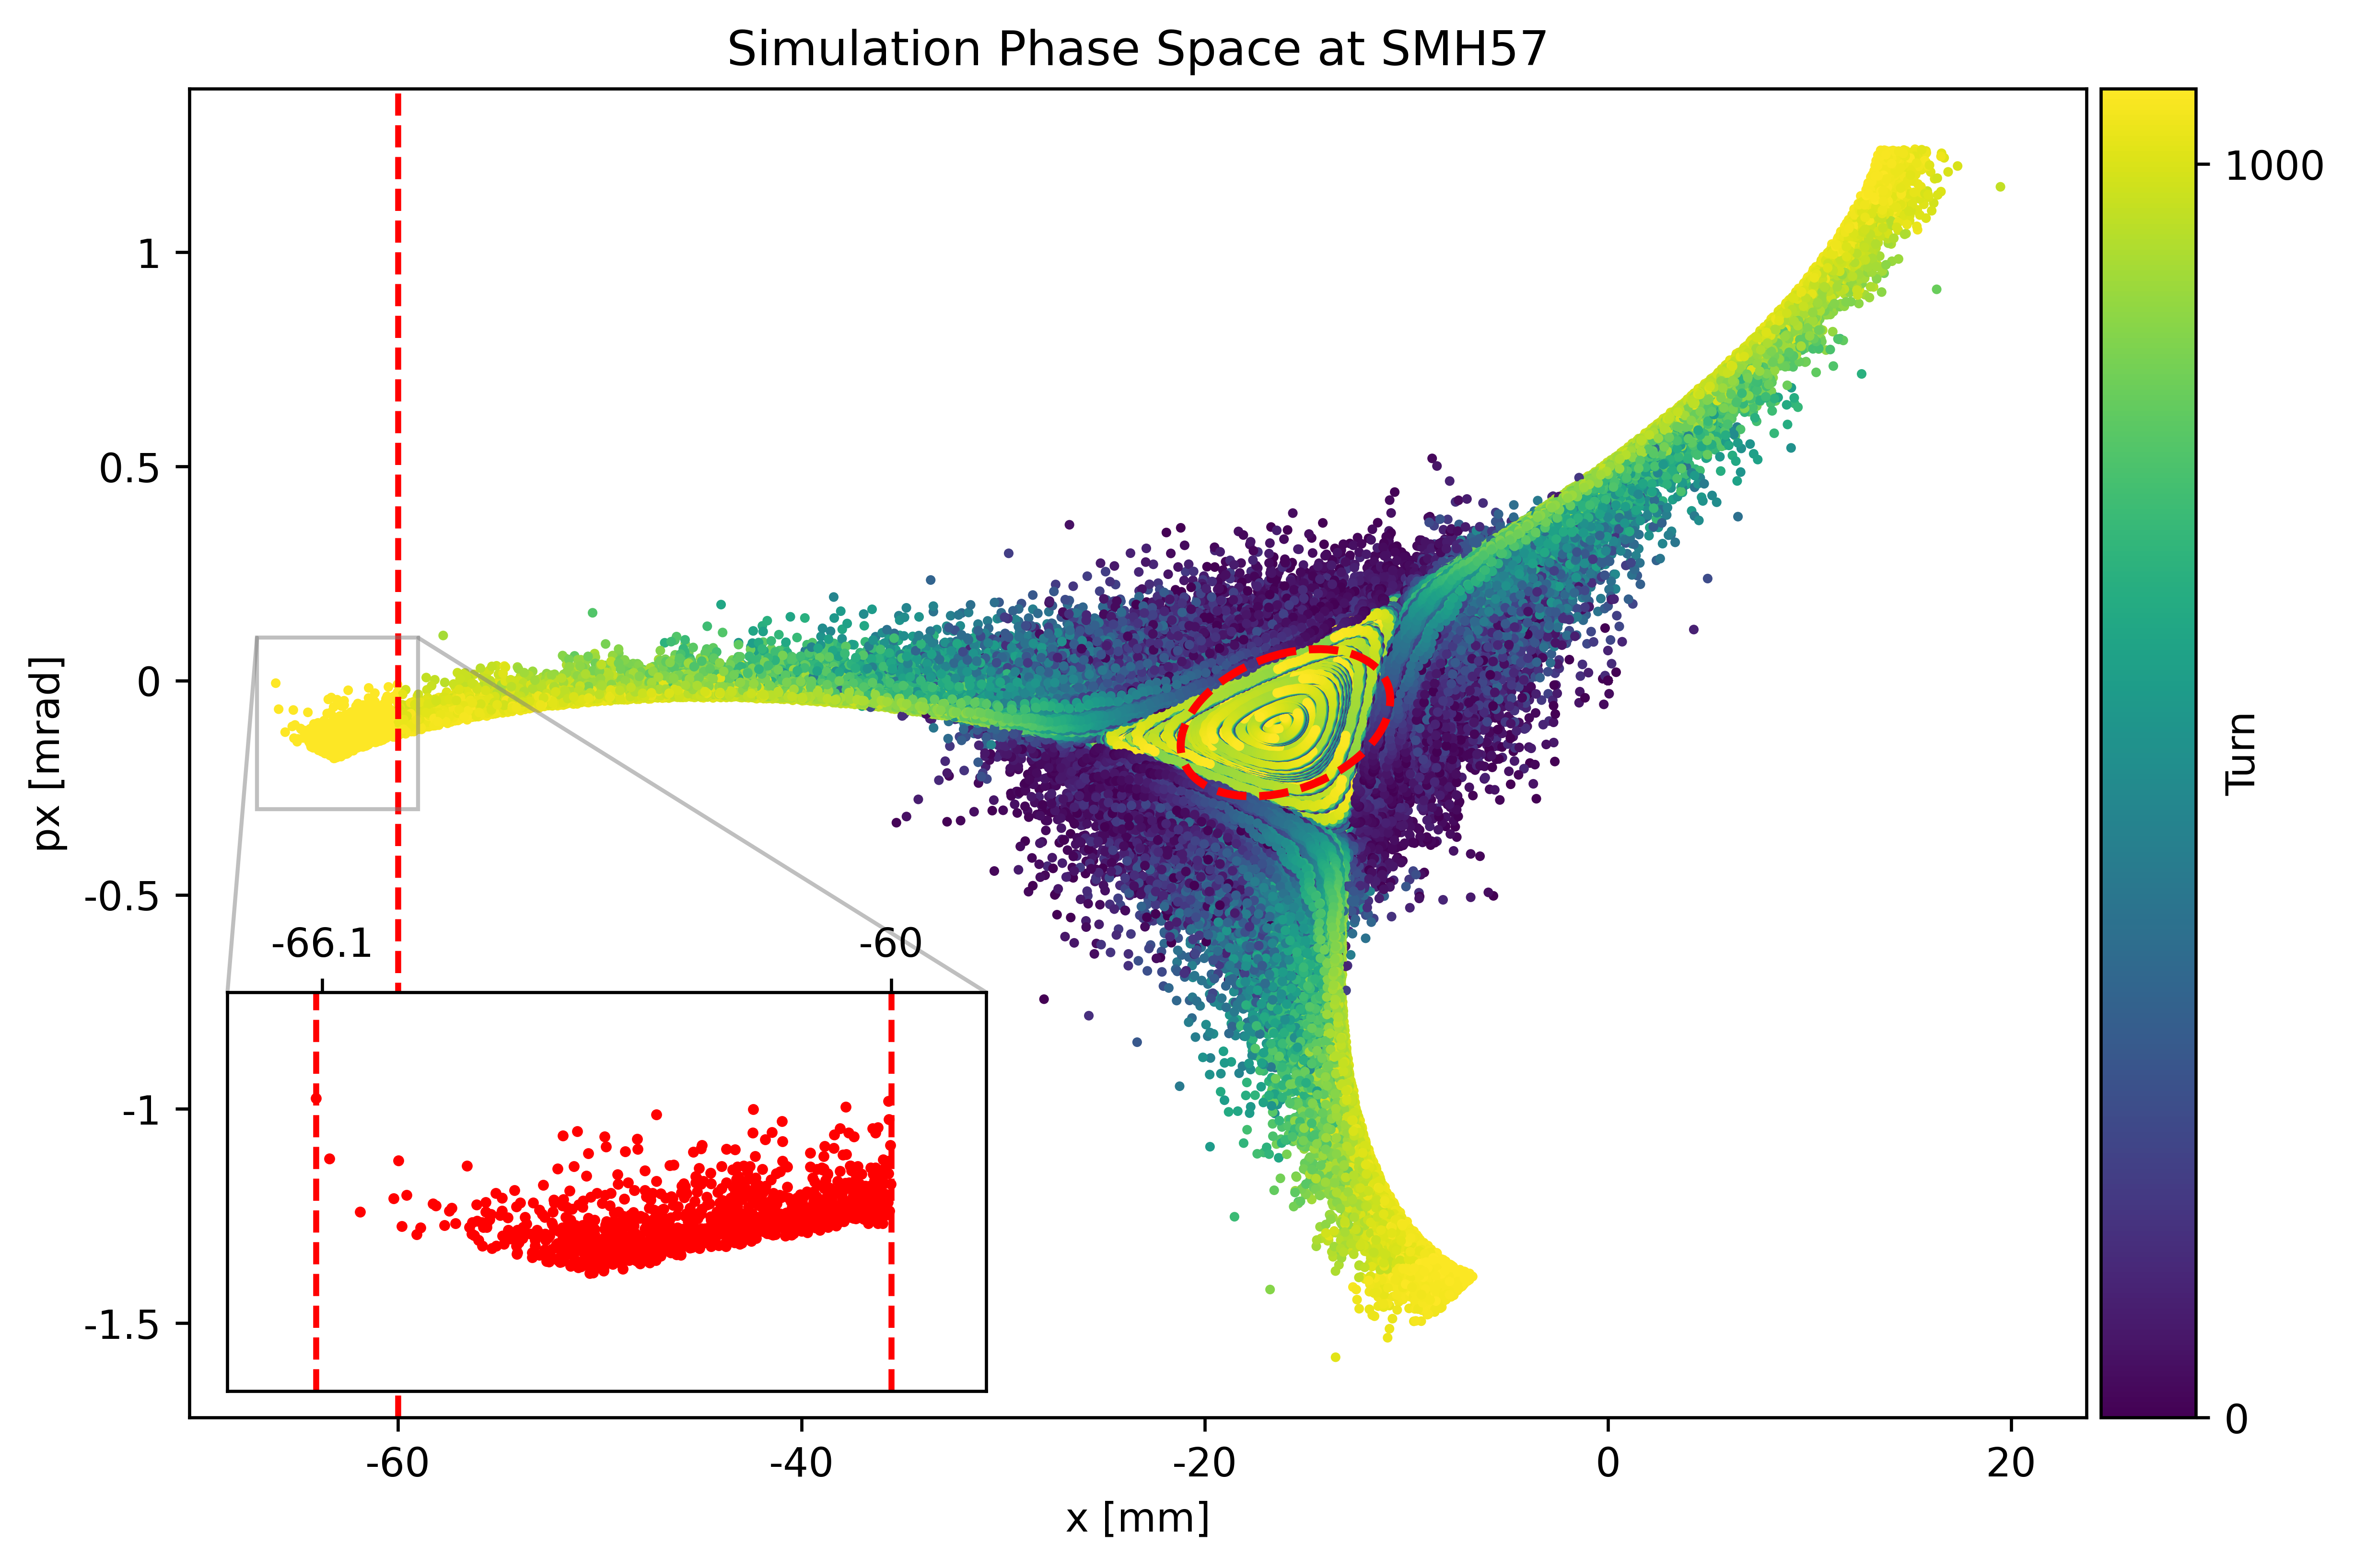
\includegraphics[width=0.9\linewidth]{phase-space-sim.png}
  \cprotect\caption{Phase-space distribution of the RFKO simulation at the \verb|SMH57| septum location, plotting all particles for the first 1000 turns (approx.\qty{2.128}{\milli\second} in laboratory time). RFKO driven by a transverse excitation frequency chirp across $f_{rev}/3$ at a \textit{rep-rate} of \qty{0.12}{\milli\second}. Color scale indicates turn number. Inset shows extracted particle distribution and a spiral step of $\Delta X_3\approx$\qty{6.1}{\milli\meter}.}\label{fig:phase-space-sim}
\end{figure}



\begin{figure}[h]
  \centering
  \includegraphics*[width=0.8\linewidth]{simulation-flowchart.png}
  \caption{A flowchart describing an overview of the simulation process}\label{fig:flowchart}
\end{figure}


\chapter{Analysis and Comparison of Results}
This chapter presents the methodology and results of experiments seeking to confirm the successful implementation of RFKO slow extraction at the PS for East Area spills. The accuracy of the simulation models will be confirmed by analysing the spill characteristics, compared between experimental data taken in June 2023 and the results of simulations. This chapter will also seek to demonstrate the benefits of GPU-accelerated particle simulations using \verb|Xsuite|, as compared to typical CPU workflows.


\section{Computation Time}

In order to compare the advantages of GPU acceleration provided by \verb|Xsuite|, the simulation process described in~\autoref{sec:sim_process} was implemented and run using CERN's batch service. The simulations used single-CPU compute nodes, either using \verb|Xsuite|'s CPU context, or GPU context with additional Nvidia GPUs via \verb|Xsuite|'s CUDA interface. Simulations were run for a range of numbers of particles and turns, and the real-time (\textit{wall-clock}) duration of the simulation was recorded. These results are presented in~\autoref{fig:cpu_graph_per_turn} and~\autoref{fig:gpu_graph_per_turn}. The number of particles in a simulation---$N_p$---effectively controls the computational intensity, as it determines the number of calculations which must be performed per iteration (turn). The number of turns---$N_t$---controls the number of iterations, and is therefore used to normalise computation time between simulation runs.

These figures show significantly different dependency of simulation process time on the operational intensity between CPU and GPU workloads. For CPU tasks there is no parallelism available, so for $N_p>10^2$---where performance isn't dominated by constant-time \textit{overhead} processes---performance is dependant on $N_p$. For GPU tasks, however, there is a significant initial overhead process of allocating and transferring data from the CPU to GPU. This is apparent from the stratification of performance (time per turn) in~\autoref{fig:gpu_graph_per_turn}. The performance, however, is not dependent on $N_p$ for $N_p<10^6$, where the performance is dominated by the constant-time parallelism available.

GPUs employ a \textit{Single-Instruction Multiple-Data} (SIMD) architecture to execute a single operation on multiple data points (\textit{vectors}) concurrently. This is in contrast to CPUs, which employ a \textit{Single-Instruction Single-Data} (SISD) architecture, where each operation is performed on a single data point at a time. This means that the GPU can perform $N_p$ operations in the same time as a CPU can perform a single operation, and so the performance is not dependant on $N_p$. The GPU constant-time performance is saturated for $N_p>10^6$, where all available parallelism is being used, and performance is once again dependant on $N_p$. Previous research has shown similar performance dependency on $N_p$ for GPU accelerated simulations~\cite{Hegglin:2239398}.

The paralellism-saturated performance of both CPU and GPU simulations can be formulated as linear relationships in log-log, using the equation
\begin{equation}
    t=\frac{N_p\ ^\alpha \times 10^\beta}{N_t}
\end{equation} where $\alpha$ and $\beta$ are some constants of the performance of a particular machine. By fitting the linear domain performance to this equation, values of $\alpha$ and $\beta$ can be estimated for particular CPU and GPUs. For these benchmark simulations, various AMD Epyc CPUs were assigned to the machines, and NVIDIA A100 40GB GPUs were used. This specific combination of hardware resulted in $\alpha_{CPU} = 0.95178, \beta_{CPU}=-4.34452$ for CPU-only simulations, and $\alpha_{GPU}=0.97671, \beta_{GPU}=-6.65887$ for GPU simulations (\autoref{fig:cpu_graph_per_turn}, \autoref{fig:gpu_graph_per_turn}).

\begin{figure}
  \centering
  \includegraphics*[width=0.77\linewidth]{CPU_graph_per_turn.png}
  \caption{Real simulation time (s) per turn for CPU workload per turn as a function of number of particles. Line color indicates number of turns simulated.}\label{fig:cpu_graph_per_turn}
\end{figure}

\begin{figure}[h]
  \centering
  \includegraphics*[width=0.77\linewidth]{GPU_graph_per_turn.png}
  \caption{Real simulation time (s) per turn for GPU workload per turn as a function of number of particles. Line color indicates number of turns simulated.}\label{fig:gpu_graph_per_turn}
\end{figure}

\begin{figure}
  \centering
  \includegraphics*[width=0.77\linewidth]{COMPARISON_graph_per_turn.png}
  \cprotect\caption{Real (\textit{wall time}) simulation time (s) per turn for CPU workload divided by GPU workload for the same $N_p, N_t$, showing the relative performance increase of GPU acceleration. All other parameters (e.g. number of compute cores) are held constant.}\label{fig:comparison_graph_per_turn}
\end{figure}

These optimisation improvements make a clear justification for the use of GPU-accelerated workflows.~\autoref{fig:comparison_graph_per_turn} shows the relative performance increase of GPU acceleration over CPU-only simulations, for the same $N_p, N_t$. In the best case, with $N_p, N_t \approx 5\times 10^4$, the GPU-accelerated simulation can be $\sim 500$ times faster than the CPU-only simulation. At more reasonable $N_p, N_t$, GPU simulations are still several orders of magnitudes faster than a CPU, and only slower at $N_p, N_t < 10^1$.

Previous work on optimising simulations slow extraction (at the SPS) achieved a simulation time of 7 hours 30 minutes (\qty{27000}{\second}) for a total of \qty{200000}{turns} and \qty{1000}{particles}~\cite[Figure 3]{Schicho:2039579}, using a similar batching process, but without the advantage of GPU acceleration. The simulation process described in~\autoref{sec:sim_process} achieved a total time of 13 minutes (\qty{779.8}{\second}) for the same number of particles and turns running on a GPU platform. This represents a $\times 34$ speed improvement.

These findings motivated the selection of parameters for later simulations. To simulate the full \qty{500}{\milli\second} extraction period requires \qty{235000}{turns} to be simulated. At this number of turns, the available GPU parallelism becomes saturated around \qty{500000}{particles}. By not exceeding this amount, the simulation can complete in a reasonable amount of time and still yield significant results.

\clearpage
\section{Frequency Response}\label{results:freq_response}

In order to compare the accuracy of RFKO slow extraction simulations to measurements taken from the implementation on the real machine, analytical tools established by previous work~\cite{Pari:2780495} were used to measure the frequency response of the RFKO system. By varying the rate at which a chirp was repeated, known as the \textit{interval frequency} or \textit{rep rate}, the resulting spill could be characterised. 

\subsection{Analysis Methodology}\label{sec:machine_freq_anal_method}

For the machine implementation, the spill was measured using an $N_2$ gas scintillator~\cite{Actis:bxscint} located in the F61 extraction line (see~\autoref{fig:schematic}). This scintillator is measured by various devices: the interface \verb|BXSCAL| was selected, which provided time-series measurements of particle counts at $\sim$\qty{18.8}{\kilo\hertz}. The spill was measured for a range of interval frequencies using an automated script interfacing with the \textit{Java API for Parameter Control} (JAPC) software at CERN. Multiple sets of data were taken for each interval frequency, for a range of peak voltages applied to the TFB kicker. 

\begin{figure}
  \centering
  \includegraphics*[width=0.7\linewidth]{raw_signal.png}
  \cprotect\caption{Example signals recorded by the \verb|BXSCAL| scintillator at various \textit{rep-rate} intervals.}\label{fig:raw_signal}
\end{figure}

Once the scripts completed, the \verb|BXSCAL| data was retrieved from NXCALS, CERN's logging database~\cite{nxcals}. This time-series scintillator provides a signal proportional to the instantaneous number of particles passing through the F61 extraction line, and can, therefore, be used as the extraction rate spill signal. An example of this data can be found in~\autoref{fig:raw_signal}, showing a range of rep-rate intervals. The time-series spill signal was then analysed using a discrete Fourier transform (DFT) to obtain the frequency response of the system. 


\begin{figure}
  \centering
  \includegraphics*[width=0.8\linewidth]{sample_rate_variation.png}
  \caption{Box-plot of the variation in sample rate of the \texttt{BXSCAL} device over the course of the measurement. Box shows the \nth{25} to \nth{75} percentile, with error bars bounding the \nth{10} and \nth{90} percentile. Data points outside of this range are considered outliers and shown as diamond points.}\label{fig:sample_rate_variation}
\end{figure}

Once the DFT was computed, the interval rate for each measurement was selected, normalised by the DFT DC component (the \qty{0}{\hertz} term, equivalent to the average of all samples). A peak-finding algorithm was used to identify this interval rate, allowing for a slight variation in the spill measurement frequency. Over the measurements used, the \verb|BXSCAL| sample rate varied between \qty{18.6}{\kilo\hertz} and \qty{18.95}{\kilo\hertz} (\autoref{fig:sample_rate_variation}). This sample rate variation likely originates from the electrical sampling equiptment, or from changes in gas pressure~\cite{PLUM200274}. As the variation was evenly distributed around the mean value of \qty{18.78}{\kilo\hertz}, the DFT was largely unaffected. The peak-finding algorithm was used to identify the highest peak within a range corresponding to the inter-quartile range of sample rate variance. An example of these DFTs, with the range and selections of the peak-finding algorithm, can be seen in~\autoref{fig:raw_ffts}.

To compensate for the ``noise'' level of the machine data---a result of the measurement device resolution, scintillator ``after-glow'', residual current (``dark current''), or readout noise---the noise level was estimated from signal regions before excitation, then subtracted from the measured frequency amplitudes. Error-bar calculations for both machine and simulation data sets were made using the variance between multiple measurements at the same parameters, the variance between all measurements, and the machine noise level.

\begin{figure}
  \centering
  \includegraphics*[width=0.8\linewidth]{raw_ffts.png}
  \caption{Example Discrete Fourier Transforms (DFT) of the spill signals in~\autoref{fig:raw_signal}. The \textit{expected} interval frequency is shown as a dashed line, and the range around which the peak-finding algorithm searched is shaded. The accepted peaks are shown in grey marks, and the selected peak is shown in red.}\label{fig:raw_ffts}
\end{figure}

This selection process was found to be robust but noisy, especially at higher frequencies, where the variation in the \verb|BXSCAL| sample rate has a higher impact on the accuracy of the DFT. To mitigate this, the peak-finding algorithm was run on multiple repetitions of the same parameters, and the results averaged.

This same analytical method was performed for simulations; the turn number at which a particle was lost to the aperture was recorded, along with its longitudinal $\zeta$ variable, defined as
\begin{equation}
  \zeta = s \frac{\beta}{\beta_0} - \beta c t
\end{equation}
where $\beta$ is the relativistic Lorentz factor. This was used to reconstruct the \textit{laboratory} time (in real seconds, not turn number) at which the particle was lost to the aperture---and thus considered as extracted---using the equation
\begin{equation}
  t = N t_{rev} - \frac\zeta{\beta_0 c}
\end{equation}
where $t_{rev}=1/f_{rev}$, the revolution time of the reference particle, and $N$ is the turn at which the particle was lost. This equation can also be found in the source code for the \verb|Exciter| element. The extraction time data for each particle was then used to reconstruct the time-series extraction data (\autoref{lst:time_series_calculation}). The same peak-finding algorithm as used for machine data was then employed to generate frequency response data for simulations.


\subsection{Results of Frequency Response Analysis}
\autoref{fig:freq_response_machine} presents the results of the analysis method described in~\autoref{sec:machine_freq_anal_method} applied to data measured from the PS. The graphs characterise the \textit{frequency response} of the spill to different chirp signal \textit{rep-rate} intervals, and indicate how this frequency propagates to the output (spill). The frequency response of the RFKO system is shown for both a bunched beam (upper image) and a coasting beam (lower image). Visible in both \textit{log-log} plots is a distinct \textit{low-pass filter} effect, where the frequency response is reduced at higher frequencies. This effect, also observed by previous studies~\cite{wepmp008,Pari:2780495}, results in higher frequencies being ``smoothed out'' by the RFKO system. 

The frequency response $H(f)$ of a low-pass filter can be approximated to the first order as
\begin{eqnarray}
  H(f) = A\cdot \frac 1{1 + \left( \frac{f}{f_c} \right)^{2n}}
\end{eqnarray}
where $f_c$ is the cutoff frequency, $n$ is the order of the filter (which determines the steepness of the roll-off), and $A$ is a gain constant. The frequency response curve at each gain was fitted to this function, and the fitted curve and variance error are shown in red in~\autoref{fig:freq_response_machine} and~\autoref{sec:machine_freq_anal_method}.

For \textbf{bunched beams}, the low-pass filter was found to have a cutoff frequency of \qty[separate-uncertainty = true]{1.14(0.173)}{\kilo\hertz} in machine measurements, and \qty[separate-uncertainty = true]{1.49(0.257)}{\kilo\hertz} in simulation. Both machine measurement and simulation fits resulted in an order of exactly 1, to 7 decimal places. These results show that the frequency characteristics of the bunched-beam RFKO simulations are accurate to the machine implementation.

For \textbf{coasting beams}, the fitted low-pass filter has a cutoff frequency of \qty[separate-uncertainty = true]{1.12(0.190)}{\kilo\hertz} in machine measurements, and \qty[separate-uncertainty = true]{5.26(1.03)}{\kilo\hertz}. While these results have a significantly larger error than the bunched beam results, they are still in agreement with each other. The filter order $n$, however, is not consistent between simulation and measurements: in simulation, the curve is fit to $n=10$, a very steep roll-off; for the machine measurements, the curve is fit to $n=1$.

Both plots also show a \textit{minimum transfer characteristic}, where the frequency response is at its lowest: for bunched beams, this minima is at \qty{4}{\kilo\hertz}, meaning a chirp signal repeating every \qty{0.25}{\milli\second} will have the least effect on frequencies present in the spill signal. For coasting beams, this minima is less clear, and appears to shift to higher frequencies with increasing chirp signal voltage.

The low-pass filter effect, and corresponding cutoff frequency and minimum transfer characteristics, can be explained by the time taken for particles to move from a stable phase-space area to the magnetic septum~\cite{Sorge_2018}. This time $T_{tr}$, in units of 3 turns, is known as the \textit{transit time}, and is given by~\cite{Pullia:313678, Bryant:CAS}:
\begin{equation}
  T_{tr} = \frac 1{\sqrt{3}{\varepsilon_Q}} \ln \left| \frac n{n+3} \frac 3{\frac {\dot {\varepsilon_Q}}{\varepsilon_Q} - \frac 1{\sqrt 3}\frac{\dot{{\varepsilon_Q}}}{{{\varepsilon_Q}}^2}}\right|
  \label{eq:transit_time}
\end{equation} 
The first fraction within the logarithm, where $n=|\vec X_{MS}|/|\vec X_{sep}|$, accounts for the time taken to move from a fixed point $O'$ to the magnetic septum, where the distance between the edge of the stable phase space area and the septum is $|X_{MS}|$, and the distance between the edge of the stable phase space area enclosed by the separatrices and its center is $|X_{sep}|$. The second fraction, where ${\varepsilon_Q}$ was defined as the modified tune distance in~\autoref{eq:spiral_step} and~\autoref{eq:spiral_kick}, accounts for time taken to move along the side of a stable triangle to the fixed point $O'$.~\autoref{fig:transit_time} illustrates this transit time in phase-space.

\begin{figure}
  \centering
  \includegraphics*[width=0.6\linewidth]{transit-time-phase-space.png}
  \caption{A phase-space diagram illustrating the transit time $T_{tr}$ elapsed between leaving the last stable triangle and arriving at the septum. The particle motion (and transit time) is presented in units of three turns; in real-time, the particle moves between the three separatrix arms. The Kobayashi Hamiltonian forms the separatrices of the stable triangle. Total transit time $T_{tr}=T_{tr,1} + T_{tr,2}$ depends both on the distance $(x_0, y_0)$ of the particle from a fixed point $O'$ ($T_{tr,1}$) and the distance from $O'$ to the septum blade ($T_{tr,2}$).}\label{fig:transit_time}
\end{figure}

In a machine with a chromatic tune spread, this transit time $T_{tr}$ will have a spread of values $\Delta T_{tr}$, which represents a time interval within which particles which leave the stable phase space simultaneously will arrive at the septum. This results in a \textit{limiting frequency} $f_{\lim}=1/\Delta T_{tr}$, above which frequencies in the spill structure are ``washed out''. 
The spread of transit times is therefore approximated to~\cite{PhysRevApplied.13.044076, Pullia:313678}
\begin{equation}
  \Delta T_{tr}\approx\frac{dT_{tr}}{d{\varepsilon_Q}}\Delta{\varepsilon_Q}\propto\frac 1{\overline{\varepsilon_Q}^2}\Delta\varepsilon_Q
\end{equation} where $\overline{\varepsilon_Q}$ is the mean modified tune distance. 
The consequence of this transit time spread is a spread in septum arrival time between instantaneously excited particles. Should the chirp repetition period be shorter than this interval, the chirp repetition frequency component will be ``washed out'' in the spill structure.

The simulated frequency response characteristics are shown in~\autoref{fig:freq_response_sim}, using the same parameter ranges as~\autoref{fig:freq_response_machine}. The bunched beam frequency response shows the same minima characteristic as the real machine, with a minimum at \qty{4}{\kilo\hertz}. The coasting beam simulations, however, do not have the same accuracy. The frequency response minima seen in~\autoref{machine_rf_off} is still present at \qty{4}{\kilo\hertz}, but the typical low-pass filter effect is not seen, with the response returning to a high level as the chirp frequency approaches \qty{10}{\kilo\hertz}.

\begin{figure}[h]
  \centering
  \begin{subfigure}[b]{0.9\linewidth}
    \includegraphics*[width=\linewidth]{machine_rf_on.png}
    \caption{Frequency response of machine measurements with a \textbf{bunched} beam.}\label{machine_rf_on}
  \end{subfigure}
  \begin{subfigure}[b]{0.9\linewidth}
    \includegraphics*[width=\linewidth]{machine_rf_off.png}
    \caption{Frequency response of machine measurements with a \textbf{coasting} beam.}\label{machine_rf_off}
  \end{subfigure}
  \caption{Frequency response of the RFKO system as implemented in the PS, both with a bunched beam (upper image) and coasting beam (lower image).}\label{fig:freq_response_machine}
\end{figure}

\begin{figure}[h]
  \centering
  \begin{subfigure}[b]{0.9\linewidth}
    \includegraphics*[width=\linewidth]{sim_rf_on.png}
    \caption{Frequency response of simulations with a \textbf{bunched} beam.}\label{sim_rf_on}
  \end{subfigure}
  \begin{subfigure}[b]{0.9\linewidth}
    \includegraphics*[width=\linewidth]{sim_rf_off.png}
    \caption{Frequency response of simulations with a \textbf{coasting} beam.}\label{sim_rf_off}
  \end{subfigure}
  \cprotect\caption{Frequency response of the RFKO system as simulated in \verb|Xsuite|, both with a bunched beam (upper image) and coasting beam (lower image).}\label{fig:freq_response_sim}
\end{figure}

\autoref{fig:simvmeas_bunched} and \autoref{fig:simvmeas_coasting} directly compare the frequency response between empirical measurements and simulations, 
for both bunched and coasting beams. These graphs present the average response curve between different voltages, and the fitted low-pass filter model, with the cutoff frequency $f_c$ marked. While less pronounced in a \textit{log-log} graph, the similarities in the response frequency for bunched beams is clearly seen in \autoref{fig:simvmeas_bunched}. For coasting beams (\autoref{fig:simvmeas_coasting}), this similarity is poorly observed, motivating the conclusion that---while the low-pass filter is still present---the coasting beam simulations were innaccurate.   

\begin{figure}[!h]
  \centering
  \includegraphics*[width=0.8\linewidth]{simvmeas_bunched.png}
  \caption{Graph comparing the averaged frequency response curves for bunched beams between machine data (black) and simulations (red). Shaded is the $1\sigma$ error, dashed is the fitted low-pass filter model, and vertical dashed is the calculated cutoff frequency $f_c$ and the $1\sigma$ error.}\label{fig:simvmeas_bunched}
\end{figure}

\begin{figure}[!h]
  \centering
  \includegraphics*[width=0.8\linewidth]{simvmeas_coasting.png}
  \caption{Graph comparing the averaged frequency response curves for coasting beams between machine data (black) and simulations (red). Shaded is the $1\sigma$ error, dashed is the fitted low-pass filter model, and vertical dashed is the calculated cutoff frequency $f_c$ and the $1\sigma$ error.}\label{fig:simvmeas_coasting}
\end{figure}

\clearpage
\section{Spill Duty Factor}\label{results:sdf}

Another analytical tool for quantifying slow extraction spill quality established by previous work is the \textit{spill duty factor}. This quantity is defined as~\cite{Sorge_2018}
\begin{equation}
  \mathcal{F} = \frac{\langle x\rangle^2}{\langle x^2\rangle}
\end{equation} where $\langle x\rangle$ denotes the average of an arbitrary variable $x$. By calculating this quantity within a rolling time window, a rolling average of spill quality can be calculated.~\autoref{fig:sdf_example} presents an example of these calculations for the spill signals in~\autoref{fig:raw_signal}: a flatter spill will produce a duty factor closer to $\mathcal{F}=1$, while a highly pulsed spill approaches $\mathcal{F}=0$.

\begin{figure}
  \centering
  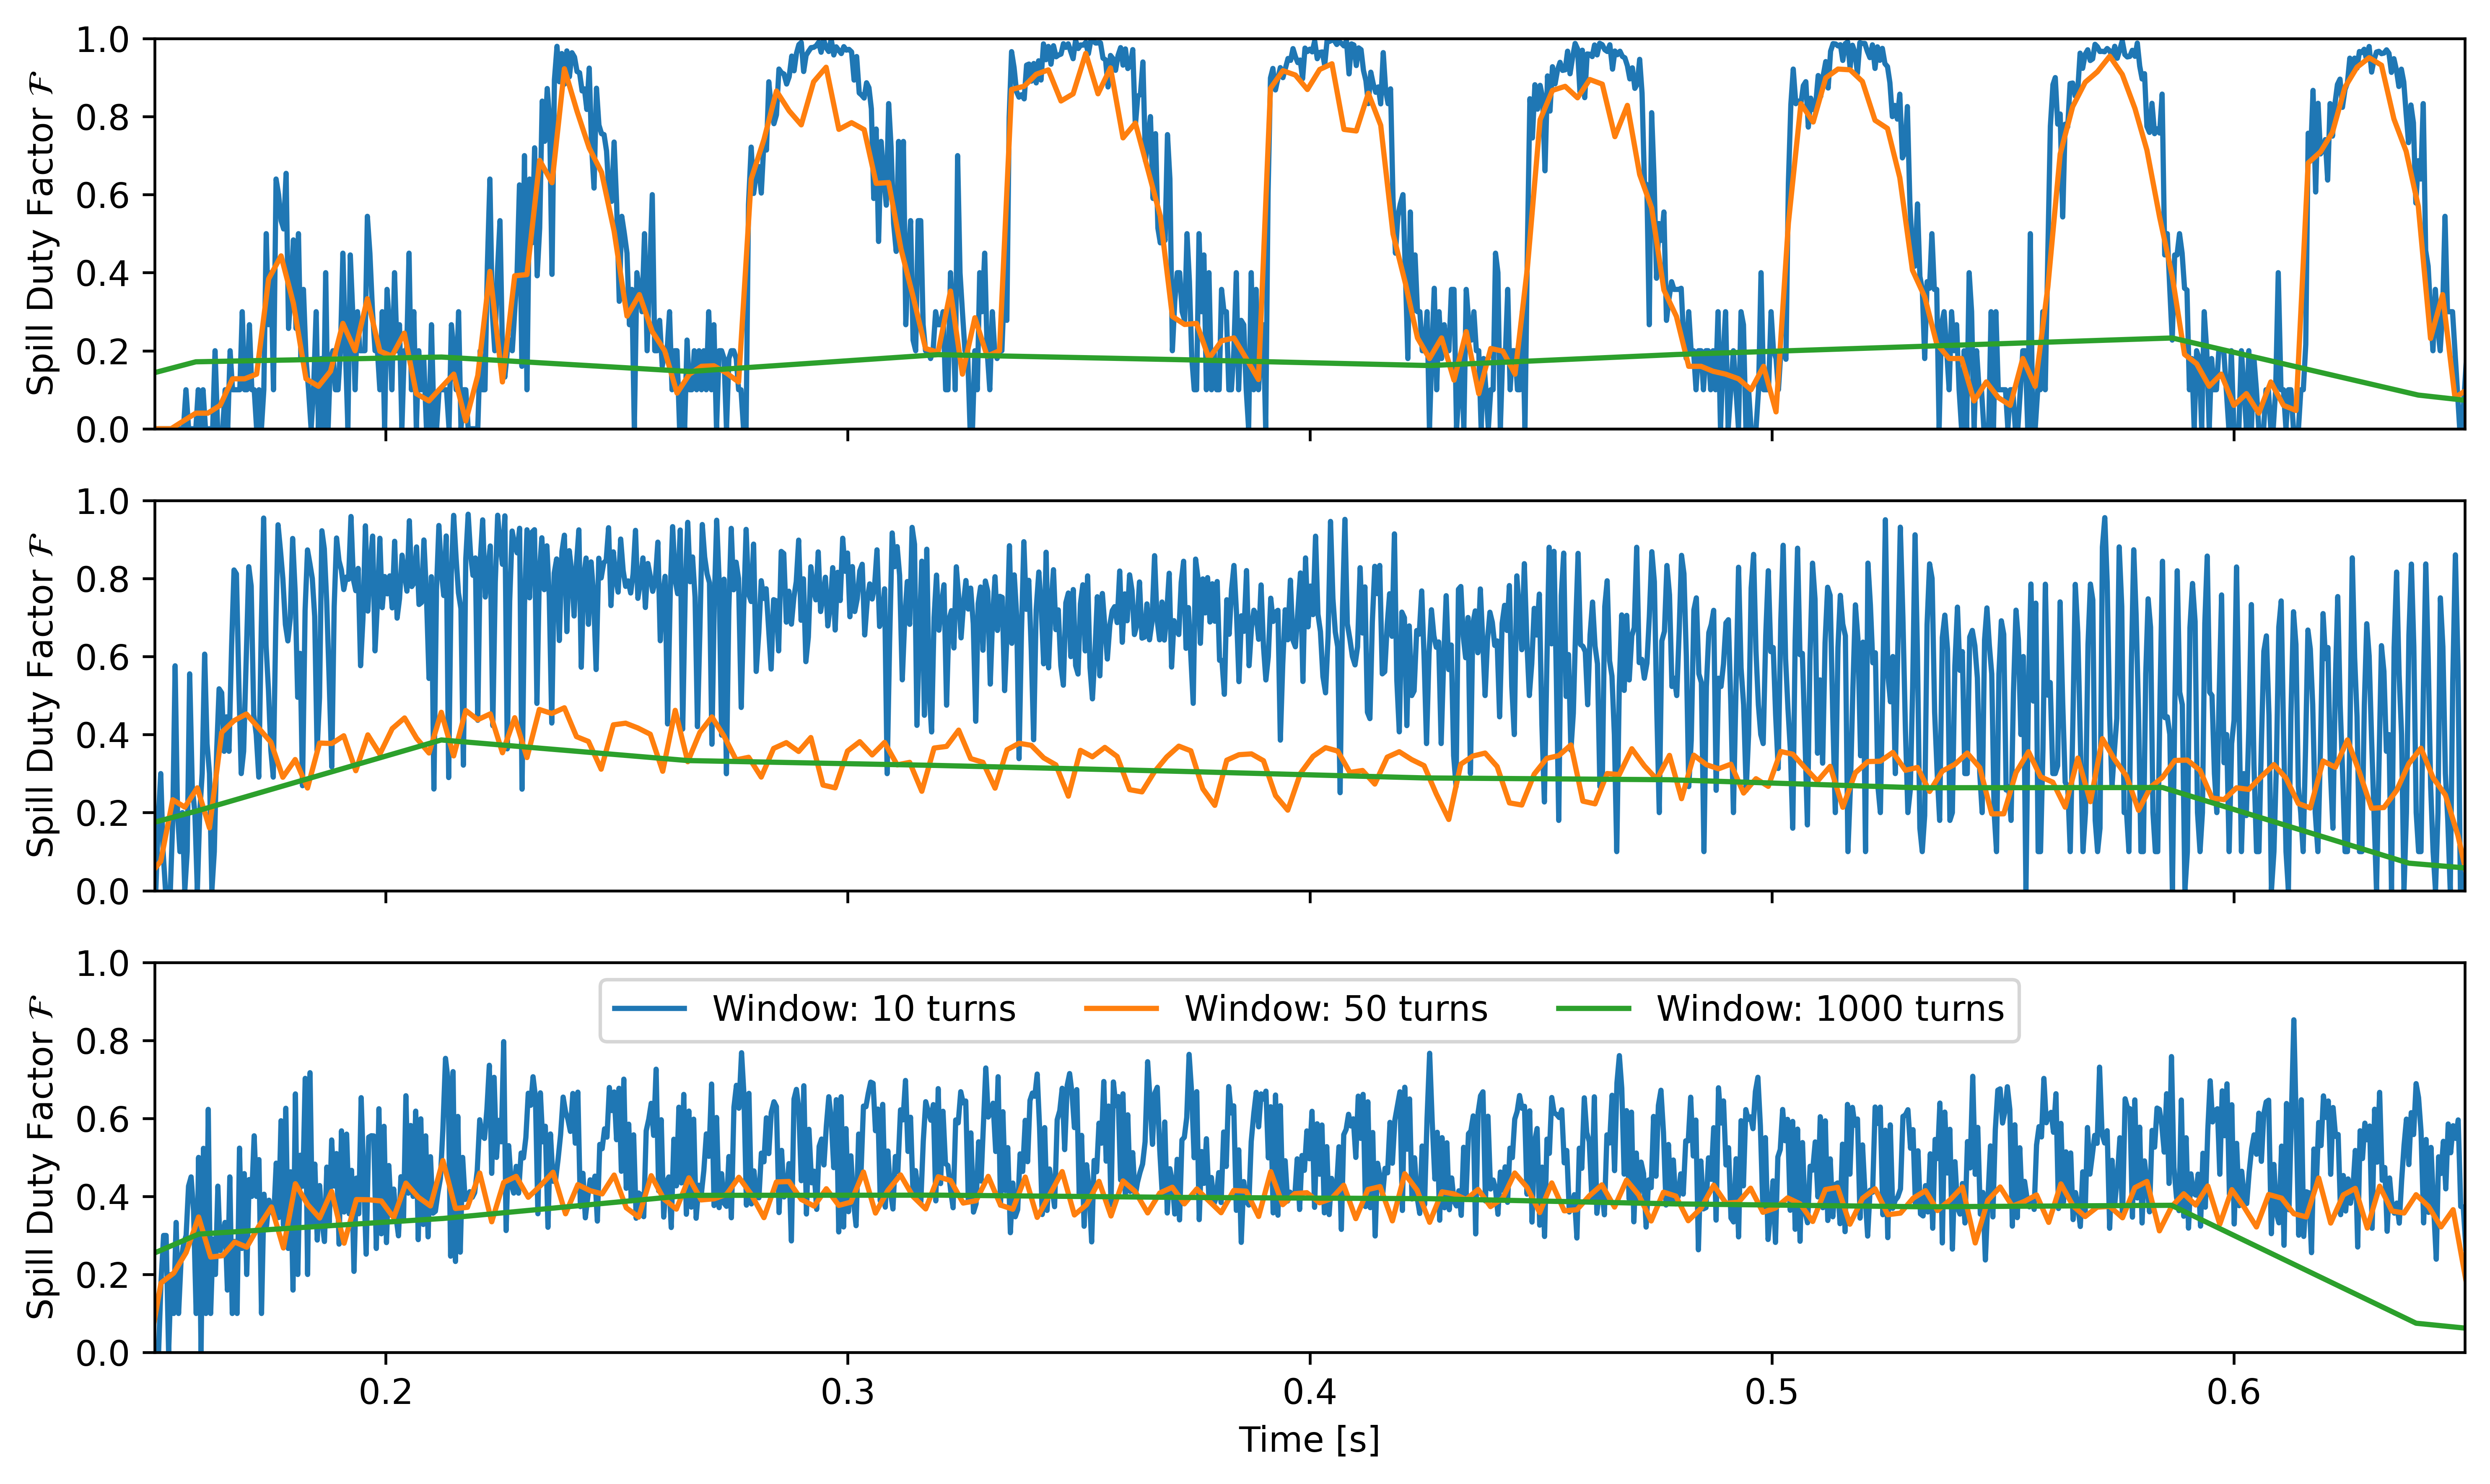
\includegraphics[width=0.8\linewidth]{sdfs.png}
  \caption{Example rolling spill duty factor ($\mathcal{F}$) of the spill signals in~\autoref{fig:raw_signal}. Calculations made with 10, 50, and 1000 turn windows.}\label{fig:sdf_example}
\end{figure}

~\autoref{fig:sdf_meas} shows measurements of spill duty factor for both bunched (top) and coasting (bottom) beam RFKO spills, over a range of TFB signal voltages and chirp repetition frequencies. These are presented in a heatmap, where the lightness of the cell represents a higher spill duty factor, and thus a flatter spill. Qualitative analysis identifies regions where the spill quality is optimised (high $\mathcal{F}$), making for optimal parameter selection. For bunched beams, the area of optimal spill quality is large, with a maximum duty factor $\mathcal{F} = 0.8$. For coasting beams, the region of optimal spill quality is much smaller, with a maximum duty factor $\mathcal{F} = 0.6$. Previous work on optimising slow extraction at the PS supports this finding of increased spill duty factor with RF cavities enabled, compared to beams with RF cavities disabled~\cite{Cappi:134321}.

The mechanism behind the spill duty factor improvement with bunching can be understood by examining how the stable phase space behaves with respect to synchrotron oscillation. As covered in~\autoref{sec:long_phase_space}, particles moving within longitudinal RF buckets will undergo longitudinal oscillations around the synchronous particle, known as synchrotron oscillations\footnote{As opposed to the transverse betatron oscillations.}. This can be calculated as
\begin{equation}
  Q_s = \sqrt{\frac{hqV_{rf}|\eta|\cos\phi_s}{2\pi\beta_0^2E_{tot}}}
\end{equation} where $h$ is the RF harmonic, $V_{rf}$ the RF voltage, $q$ the particle charge, $\eta$ the slip factor (\autoref{eq:slip_factor}), $\phi_s$ the synchronous phase, and $E_{tot}$ the total energy. It can also be found by simulation; for the configuration outlined in preceding sections, the synchrotron tune was found to be $Q_s = 0.0052$. 
In a Steinbach diagram (\autoref{sec:steinbach}), this has the effect of shifting the particle horizontally, in addition to the vertical push from the exciter. This has two consequences: the particles remain at the edge of the unstable region for a shorter amount of time, as the synchrotron motion changes the particle's tune enough to move it into resonance, reducing the effect of the excitation structures. Additionally, it can reduce the effect of magnet ripples changing the shape of the unstable region.

\begin{figure}[h]
  \centering
  \includegraphics*[width=0.66\linewidth]{synch-phase-space.png}
  \caption{Phase space of a particle approaching the separatrix in a coasting beam (top) and a bunched beam (bottom), both with a small sextupole ripple component.}
  \label{fig:synch-phase-space}
\end{figure}

To see this, we will consider the two cases of a particle approaching resonance in a coasting beam and in a bunched beam, visualised in phase space in \autoref{fig:synch-phase-space}. The upper figure is the case for a coasting beam with no synchrotron motion: particles experience no change in tune, and so a small ripple in sextupole field could increase the stable region area and ``recapture'' the particle back into the stable region, preventing the particle's extraction. The lower figure describes the case for a bunched beam with slow synchrotron motion: the particles receive a kick (RFKO) \textit{and} and periodic tune change (RF cavity), which reduces the stable phase space area. This reduces the chance of a particle being recaptured by a sextupole ripple, pushes the particle deeper into resonance quicker, and ``smoothens'' out the spill signal. There is, however, a limit to this ripple mitigation, where the synchrotron oscillation is too fast for particles to remain in the unstable region.~\cite{Sorge_2018,PhysRevAccelBeams.26.014402}.

This synchrotron motion also effects the extraction transit time. The distance of a particle from the separatrix while in the unstable region grows with each synchrotron period. This reduces the transit time. Therefore, there exists an optimum synchrotron tune, where particles are more likely to remain within the unstable region, but the transit time remains long enough to smoothen the spill ``pulses'' between successive excitations (\autoref{fig:sdf_example}). Both of these effects, and the limiting frequency obtained from transit time spread, contribute to the optimal selection of parameters for an RFKO driving signal.

\begin{figure}[h]
  \centering
  \begin{subfigure}[b]{0.9\linewidth}
    \includegraphics*[width=\linewidth]{sdf_on_meas.png}
    \caption{Spill duty factor heatmap for \textbf{bunched} beam as measured in the machine.}\label{sdf_on_meas}
  \end{subfigure}
  \begin{subfigure}[b]{0.9\linewidth}
    \includegraphics*[width=\linewidth]{sdf_off_meas.png}
    \caption{Spill duty factor heatmap for \textbf{coasting} beam as measured in the machine.}\label{sdf_off_meas}
  \end{subfigure}
  \cprotect\caption{Spill duty factor ($\mathcal{F}$) heatmaps for the RFKO system as measured in the machine, both with a bunched beam (upper image) and coasting beam (lower image), as a function of chirp repetition frequency (log-scale) and voltage (linear). Color scale represents $\mathcal{F}$.}\label{fig:sdf_meas}
\end{figure}


\chapter{Conclusion}

This thesis presents a number of developments towards the operational implementation of Radio Frequency Knockout (RFKO) slow extraction at CERN's Proton Synchrotron (PS) for the East experimental area (EA). Within the goal of producing low intensity, high charge, high energy, and long duration spills for fixed target experiments, the implementation of RFKO presented shows promising spill frequency structure and duty factor performance. The results of machine studies presented in~\autoref{results:freq_response} and~\autoref{results:sdf} use both time-domain and frequency-domain analysis to show that the system is capable of producing spills with a flat frequency structure at durations significantly longer than \qty{100000}{turns}, and with spill duty factors of up to \qty{80}{\percent} for bunched beams, and \qty{60}{\percent} for coasting beams.

This thesis also demonstrates significant agreement between the frequency response of this RFKO implementation and the characteristics observed in previous studies~\cite{wepmp008,Pari:2780495}. This agreement is also well-observed between the real machine and simulations with a bunched beam, where both datasets place the optimum repetition frequency (minimising the presence of this frequency in the spill) for a RFKO-driving chirp signal between \qty{2}{\kilo\hertz} and \qty{4}{\kilo\hertz}. This finding motivates the development of a dedicated signal generator for the PS TFB system for use with RFKO. 
This agreement is less well-observed for coasting beams, where the simulations show lower frequency response minima than machine observations. 

The implementation of RFKO simulations in \verb|Xsuite| presented in~\autoref{sec:rfko_sim} also show significant performance improvements over previous work simulating Slow Extraction at the SPS with \verb|MAD-X|~\cite{Schicho:2039579}. By exploiting GPU accelerated computing provided by \verb|Xsuite|'s compatibility with \verb|CuPy|, CERN's batch-processing service, and containerised environments, the simulations presented in this thesis are up to 400 times more performant in real-world simulation time than CPU-based methods.

\section{Outlook}

There are several opportunities for improvements presented in this thesis, both for potential future studies, and for the operational implementation of RFKO at the PS:
\begin{itemize}
  \item As mentioned in~\autoref{sec:septum}, only one of the magnetic septa---\verb|SMH57|---was modelled for extraction. The accuracy of the simulation model would benefit from future development to simulate particles through both the septa and into the F61 line. This would require combining the PS optics models with the \textit{F61} optics models provided by \textit{acc-models-tls}~\cite{optics_repo}.
  \item The setup of the AFG used to generate chirp signals with repetition rates below \qty{1}{\milli\second} (\autoref{sec:magcycle}) was only a temporary solution, and is not suitable for long-term operational use, as it operates entirely independently from the LHC Software Architecture~\cite{Roderick:1215575} (LSA) database. A dedicated signal generator, with an interface to CERN's Technical Network and LSA would be a significant improvement.
  \item The extraction procedure outlined in this thesis only used frequency-modulated chirp signals to sweep across the range of particle tunes. Other work has used signals such as coloured noise~\cite{Nagaslaev:2011zz}. These signals, and others such as dual-band frequencies, could be explored in future studies, using the same equipment and methods as presented in this thesis.
  \item In addition to frequency-modulation control, amplitude-modulation control has been studied in the past, and can offer improvements in macro-scale spill structure~\cite{NODA2002241}. This technique could be used to mitigate the exponential decay seen in all spill structures presented in this thesis, and extend spill times to durations significantly longer than \qty{0.5}{\second}.
  \item While simulations for bunched beams show good agreement with the machine implementation, the results of coasting (debunched) beams are less clear. The longitudinal dynamics of the coasting beams in RFKO would require further characterisation to fully understand the differences between the simulations and the machine.
\end{itemize}


\chapter{Acknowledgements}
% This work, and my research over the past 12 months at CERN, would not have been possible without the tutelage and support of my studentship supervisor, Yann. I cannot thank him enough for his patience and guidance in turning a Bachelors student---without any formal background in Accelerator Physics---into a Master's candidate. I would also like to thank Matthew for his endless knowledge and assistance with my research and machine operation. 

% I am also deeply grateful to my section colleagues---Eliott, Pablo, Francisco, Vittorio, and Rebecca R.---for their friendship and for welcoming me so warmly to ABT-BTP, my section and group leaders---Chiara and Wolfgang, colleagues across the campus---Emily, Rebecca T., and the ABP, RF, BI, and OP-PS groups---and from among the wider community for their discussions, advice, and knowledge throughout my time at CERN. I would also like to thank my academic supervisor, Stephen, for his encouragement to pursue this project.

% Finally, and by no means the least, I would like to thank my family, friends, and loved ones for their support from many hundreds of miles away.
% \bibliographystyle{IEEEtran} 
\bibliographystyle{abbrvurl}
\bibliography{refs} 

\begin{appendices}

% \chapter{Derivations}

% \section{Relating longitudinal variables}

% In order to relate the dispersive and chromatic functions produced by \verb|MAD-X| to those calculated by \verb|Xtrack|, we must multiply \verb|MAD-X|'s results by the relativistic Lorentz factor $\beta=v/c$. This is because \verb|MAD-X| uses the relative momentum error $\delta_p$ as a longitudinal variable, defined as
% \begin{equation}
% \delta_p=\frac{p-p_0}{p_0}
% \end{equation}, where $p$ is the momentum of the particle, and $p_0$ the momentum of the {\it reference} (or {\it design}) particle, whereas \verb|Xtrack| uses the relative energy error

\chapter{Code Snippets}

\lstinputlisting[language=python, label={lst:kick_angle}, caption=Python code to calculate angle kick produced by the TFB system (\autoref{sec:trans_exc}).]{code/kick_angle.py}

\lstinputlisting[language=python, label={lst:generate_chirp}, caption=Python code to generate a single chirp signal as produced by the Arbitrary Function Generator (\autoref{eq:both-chirps}).]{code/generate_chirp.py}

\lstinputlisting[language=python, label={lst:time_series_calculation}, caption=Python code used to calculate the laboratory time of particle extraction and reconstruct the time-series spill array (\autoref{sec:machine_freq_anal_method}).]{code/time_series.py}

\end{appendices}

\end{document}
